% !TEX TS-program = pdflatex
% !TEX encoding = UTF-8 Unicode

%%\documentclass[preprint,review,12pt,authoryear]{elsarticle}

%% Use the option review to obtain double line spacing
\documentclass[authoryear,preprint,review,12pt]{elsarticle}

%% The amssymb package provides various useful mathematical symbols
%\usepackage{amssymb}
\usepackage{amsmath, amsfonts, amsthm, amssymb} 
\usepackage{lineno}
%\usepackage{array}
%\usepackage{mathptmx}

%% Additional packages
% tables
\usepackage{booktabs} % for much better looking tables
\usepackage{longtable}
\usepackage{multicol} % multiple columns in tables
\usepackage{multirow} % multiple rows in tables
\usepackage{rotating} % sideways tables
\usepackage{framed, color}
\usepackage[dvipsnames,table]{xcolor}
% Rotate elements in a table
\usepackage{adjustbox}
\newcolumntype{R}[2]{%
    >{\adjustbox{angle=#1,lap=\width-(#2)}\bgroup}%
    l%
    <{\egroup}}
\newcommand*\rot{\multicolumn{1}{R{90}{1em}}}
% figures
\usepackage{import} % import figures created in inskape
\usepackage{tikz} % draw figures exported from R
\usepackage[percent]{overpic} % needed for graph composition
%% bib
%\usepackage[nosectionbib, tocbib, unnumberedbib]{apacite} %% APA citation style

\journal{Energy and Buildings}

\begin{document}

\begin{frontmatter}

%% Title, authors and addresses

%% use the tnoteref command within \title for footnotes;
%% use the tnotetext command for theassociated footnote;
%% use the fnref command within \author or \address for footnotes;
%% use the fntext command for theassociated footnote;
%% use the corref command within \author for corresponding author footnotes;
%% use the cortext command for theassociated footnote;
%% use the ead command for the email address,
%% and the form \ead[url] for the home page:
%% \title{Title\tnoteref{label1}}
%% \tnotetext[label1]{}
%% \author{Name\corref{cor1}\fnref{label2}}
%% \ead{email address}
%% \ead[url]{home page}
%% \fntext[label2]{}
%% \cortext[cor1]{}
%% \address{Address\fnref{label3}}
%% \fntext[label3]{}

\title{Allocating heat consumption of residential buildings in space with help
    of a filter array to determinate the building type in a digital cadaster}

\author[HCU]{M. Esteban Mu\~{n}oz H.\corref{cor1}}
\ead{marcelo.hidalgo@hcu-hamburg.de}
\author[HCU]{Ivan Dochev}
\ead{ivan.dochev@hcu-hamburg.de}
\author[HCU]{Irene Peters}
\ead{irene.peters@hcu-hamburg.de}
\cortext[cor1]{Corresponding author}

\address[HCU]{HafenCity Universit\"{a}t, Hamburg, DE}
  %Technical Urban Infrastructure Systems Group,

%% use optional labels to link authors explicitly to addresses:
%% \author[label1,label2]{}
%% \address[label1]{}
%% \address[label2]{}

\begin{abstract}
In this paper we present a method to allocate heat demand of residential
buildings in space. The buildings and their characteristics are available from
the city digital cadaster.\\

Based on the building characteristics an appropriate \textit{building type} is
selected.  In Germany the use of building typologies for the estimation of heat
demand is a common practice.  Nonetheless this practice requires the user to
make a subjective decision regarding the choice for a type of building.  In
this paper we present a method to automatically determinate the building type
given some characteristics of the buildings and a define typology.  This method
allows us to: (1) systematically compare results of different building
typologies; (2) process large amount of building data from a digital cadaster
without binding the method to the cadaster data structure, making the method
transferable to other cities with a digital cadaster; and (3) because the
nature of our method is stochastic, we are able to represent not only a best
estimate of heat demand but the corresponding uncertainty level of the area and
of the typology.  \\

We expect to expand this method for the use of urban typologies able to
estimate and allocate heat demand of urban morphologies without the need of a
digital cadaster, expanding so the accessibility to this method to a global
scale.\\

The presented results in this paper have shown that: (1) national typologies
under estimate heat demand of the single buildings in the selected urban area,
while typologies developed for specific regions over estimate heat demand of
the same urban area; (2) national typologies perform better at an aggregated
level, while regional typologies perform better at a micro level (3) an
identification of ``hot spots'' in small urban areas is possible.  (4) for a
comprehensive identification of retrofit areas in urban spaces we need to
integrate: (a) the tertiary sector and (b) possible heat sources that can
supply the demand of these ``hot spots''.
\end{abstract}

\begin{keyword}
    Digital Cadaste \sep Residential Heat Demand \sep Building Typologies \sep
    Building Stock
\end{keyword}

\end{frontmatter}
\begin{linenumbers}

\section{Estimation heat demand for small urban areas}

The planing of cities and the planning of the underlying infrastructure to
support the demand of the individual buildings is a challenge for both: urban
planners and infrastructure planners. In this paper we discuss the first step
into a knowledge base urban planning schema. In order to achieve such a
planning schema we need information about the urban areas, here we present an
approach to classify the building stock for the estimation of heat demand.\\

We want to provide a \textbf{reprodusible} and \textbf{flxible} method for the
estimation of heat demand of urban areas at a low aggregation level. In this
paper we describe our first attempt to produce such method. In order to make
the method reproducible we create a github repository containing all the
require scripts to reproduce the presented computations and the data used in
this analysis. The provided data had to be decouple from its spatial reference
to ensure anonymity. We also provide an Ipython notebook containing step by
step explanations on how to reproduce the classification process and estimation
of heat demand with the provided scripts. All this data can be found under the
link: \url{https://github.com/emunozh/btyp}\\

In order to ensure flexibility we have constructed our set of scripts so that
these scripts can be expanded to incorporate new parameters and new functions.
The definition of individual typologies are hard coded into individual python
files. The addition of new typologies would require to only provide a new
python file. In order to facilitate this process we also provide a small script
to generate a base typology for the easy generation of new typologies.\\

We present a method for the estimation of heat demand of small urban areas at a
low aggregation (individual buildings). For this estimation we make use of
building typologies which provide us with a specific heat demand for each
building type. Because the use of urban typologies is central for this
endeavour we present a comparison of different building typologies used for the
estimation of heat demand in space. In this paper we compare and asses the
performance of this typologies.\\

We divide the paper into three main sections: (1) Section~\ref{sec:Btype}
describes the used typologies and the general structure and use of building
typologies. This section focus on German typologies but mentions also the use
of building typologies for other European countries; (2)
Section~\ref{sec:class} presents the developed method for the classification of
the buildings stock; and (3) Section~\ref{sec:result} presents and discuss the
performance of the individual building typologies presented in
Section~\ref{sec:Btype}.\\

\section{The Use of Building Typologies in Energy- and Urban-
Planning}\label{sec:Btype}

For our analysis we compare 5 typologies:
(1) \textbf{Blesl}, a simplyfied typology developed by
\citeauthor{Blesl.2007};
(2) \textbf{IWU-de}, a typology developed for Germany by the IWU\footnote{IWU
    Institut Wohnen und Umwelt GmbH \url{http://www.iwu.de}} institute;
(3) \textbf{IWU-he}, a typology developed for the federal state of Hessen by
the IWU institute;
(4) \textbf{BSU}, a typology developed for the city of Hamburg by the
BSU\footnote{BSU (Behörde für Stadtentwicklung und Umwelt) Ministry of Urban
    Development and Environment\url{https://www.hamburg.de/bsu/}}; and
(5) \textbf{EcoFYS}, a typology developed for the city of Hamburg by the
consultancy firm EcoFYS\footnote{EcoFYS\url{http://www.ecofys.com/}}.
In the following section we present an discuss this building typologies. We
start with a typology developed at a national level (IWU-de, see
Sub-Section~\ref{sub-sec:IWU-de}), this is the most used typology in Germany
for the estimation of heat demand of the building stock.  The second example is
a derivation from the fist typology.  The German typology developed by the IWU
institute is calibrated for the use of this typology to the specific federal
state of Hessen (see Sub-Section~\ref{sub-sec:IWU-he}).  With our method we
want to show how this different typologies behave for the use of small urban
areas in the city of Hamburg.  It is expected that the typology developed for
Germany will perform better than the one calibrated for the building stock of
Hessen.  We go further with our analysis and analyse two different typologies
specially developed for the city of Hamburg, expecting them to perform much
better by the analysis of a small urban area of the city.  The difference
between these typologies is the level of detail of both typologies.  While the
first typology developed my the Ministry of Urban Development and Environment
(BSU) presents a strong simplification of a typology (see
Sub-Section~\ref{sub-sec:BSU}), giving only specific heat demand of the
buildings based on two parameter:
(1) construction age; and
(2) construction type.
The second typology, developed for the city of Hamburg, delivers a
comprehensive technical report (see~\cite{Hermelink.2011}) from which many
parameters for the building classification can be derived (see
Sub-Section~\ref{sub-sec:ecofiz}).\\

In order to present a complete overview of the building typologies we make a
short review of the building typologies at an European level, driven by the
European initiative TABULAR (see Sub-Section~\ref{sub-sec:tabular}).  This sub
section also serves to build a steeping stone towards a systematic approach to
building typologies and the implementation of them in energy and urban planing
at a European and global level.  In our final remarks of the paper we revisit
the use of building typologies at an European level to highlight our envisioned
next steps.  (see Sub-Section~\ref{sub-section:next})\\

There are many building typologies for a lot of different regions all over
Europe, a good overview of the available building typologies in Europe, driven
by the TABULAR initiative, is provided in~\cite{TABULAProjectTeam.2010}.  In
Germany there are many examples of this typologies calibrated for specific
regions or cities.  (e.g.  D{\"u}sseldorf~\cite{ebok.2005};
M{\"u}nster~\cite{Hildebrandt.2003}; Freistaat Sachsen~\cite{ebok.2000};
Mannheim~\cite{ebokifeu.1998}; and Heidelberg~\cite{ebokifeu.1996}) Nonetheless
just a few have reached a scientific discussion, finding a way into the
scientific literature, few examples of this are:~\cite{Kragh.2013,
    Singh.2013, Hrabovszky.2013, Caputo.2013}.
Most of the developed typologies are developed as technical reports or
brochures targeting real state developers or home users, specially in
Germany.\\

We have structure the paper into 3 main sections.  In the first section we
present an overview of different building typologies used in Germany and
Europe.  In the second section of the paper we present our approach to
automatize the classification of the building stock, introducing the concept of
an array filter that will allocate the building types to the building stock in
a stochastic manner.  In the third and last section we present the results from
the postulated filter array and compare the results with monitoring consumption
for the same area.\\

The use of building typologies is used to estimate different retrofit scenarios
for single buildings promoting so energy-efficient measures trough the building
stock~\cite{Kragh.2013, Singh.2013, Dascalaki.2011,
TABULAProjectTeam.2012}, the use of building typologies finds also use at
estimating the mitigation potential and vulnerability of the residential
building stock~\cite{Hrabovszky.2013}.  Through the literature weAA
also find approaches addressing the issue at a urban
scale~\cite{Caputo.2013}, these approaches make use of GIS systems for the
systematic collection of building information and further classification of the
building stock.  The collection of building data in GIS systems present an
interesting tool for the analysis of urban setting rather than the analysis of
individual buildings of the analysis of the national building stock at an
aggregated level.  Nonetheless a big problem of such an approach is the
intensive data recovery needed to fill the building database.  The aim of this
paper is to develop and analyse a method that can deal with missing data in
such databases.\\

The main difference between an analysis of the national building stock, for
which the building typologies are develop, and an analysis of new decentralized
energy supply systems, which is the scope of our research, relies on scale.
While the first analysis focus exclusively on the aggregated effect of energy
efficiency measures of the building stock, the planning of decentralized energy
supply needs to:
(1) allocate the heat demand on small urban areas, suitable for small
decentralized energy supply systems; and
(2) identify \textit{heat spots} in urban areas in order to allocate retrofit
priorities.
For the proper dimensioning of heat supply systems the estimation of heat
demand demand is a key issue, specially at a low aggregation level.  The use of
building typologies for the simulation of heat demand improves as the number of
buildings are sum together~\cite{Blesl.2007}, this is because many key
parameters like internal heat gains, internal temperature, ventilation rates,
thermal bridges, etc, cannot be recover for every single building.  In order to
perform the heat demand computation the authors have to use average values
define in national guidelines.  For the construction of the typology the author
classify the buildings by its construction epoch and its construction type
(single family house, terrace house, etc.). This type of classification is a
standard in the construction of building typologies~\cite{Ebel.1990,
    ebokifeu.1996, ebokifeu.1998, ebok.2000, ebok.2005, Hildebrandt.2003,
    IWU.2003, Loga.2011, BSU.2011, Hermelink.2011, Kragh.2013,
    Singh.2013, Hrabovszky.2013, Caputo.2013}\\

An example of such an approach can be seen in Table~\ref{tab:BW}, this approach
does not use a building stock database for its construction, neither uses real
consumption data for its construction.  The construction of such a typology is
based on average parameters taken from national guideline VDI
3807~\cite{VDI-3807.1994}.  Not only for heat demand a simulation at a low
aggregation level is important.  We see a trend towards decentralized heat and
electricity production~\cite{KEMA.2012}, driven mainly by the expansion of
renewable energies.  High temporal simulation of energy signatures of small
urban areas for on site generation may be an key development towards low energy
demand neighborhoods~\cite{Koch.2013}.  In order to perform, either a simple
energy balance of the individual buildings of or a height temporal thermal
simulation models, the input data of the buildings has to be available.
Although digital cadaster data sets offer a vast amount of information of the
individual buildings, needed U-values of the building components are not
available in the digital cadaster of the city of Hamburg
ALKIS\footnote{ALKIS~\cite{adv.2008}
\url{http://www.hmdk.de/trefferanzeige?docuuid=AB8C6B21-BAFF-4230-A686-0C918FEBEE2F}}.
The use of building typologies to fill this information gap may been an
interesting option.\\

\begin{table}[htbp]
  \centering
  \caption{Building matrix with specific parameters of
  buildings}\label{tab:BW}%
    \begin{tabular}{l r rrrrrrrr}
    \addlinespace
    \toprule
    &
    \begin{sideways}\textless~1918	\end{sideways}&  
    \begin{sideways}1919--1948   \end{sideways}&  
    \begin{sideways}1949--1957   \end{sideways}&  
    \begin{sideways}1958--1968   \end{sideways}&  
    \begin{sideways}1969--1978   \end{sideways}&  
    \begin{sideways}1979--1983   \end{sideways}&  
    \begin{sideways}1984--1995   \end{sideways}&  
    \begin{sideways}1996--2000   \end{sideways}&  
    \begin{sideways}2001--2005   \end{sideways}\\
    \midrule
EFH$^a$&167&  150&  176&   150&   165&165& 156& 101&  72\\
RDH&    152&  141&  175&   162&   192&171& 129&  89&  70\\
KMH&    180&  167&  117&   191&   169&125& 101&  94&  65\\
GMH&    187&  185&  169&   148&   145&116&  82&  73&  51\\
HH &       &     &     &   103&   117&   &    &    &     \\
    \bottomrule
    \addlinespace
    \end{tabular}\\
    \begin{footnotesize}    
    source:~\cite{Blesl.2007}.
    (a) Specific Heat demand (spez. W\"armebedarfskennzahl)
    $[kWh/m^{2}a]$\\
    (EFH) Single family house ``Einfamilienhaus'';
(RDH) Terrace house ``Reihenhaus'';
(KMH) Small apartment house ``Kleines Mehrfamilienhaus'';
(GMH) Large apartment house ``Großes Mehrfamilienhaus'';
(HH) High-rise ``Hochhaus'';
    \end{footnotesize}
<<<<<<< HEAD
\end{table}
=======
\end{table}
>>>>>>> 36a956db0f2ffb15b4b8091da9293464a1b25a0c


In this paper we do not perform any calculation of heat demand, the aim of this
paper is to compare the performance of different building typologies on a small
urban area and to present our first efforts towards a systematic process to
automatize the classification of the building stock into building typologies.
The method presented in this paper could be expand into an individual building
heat balance method.\\

\subsection{IWU-de --- a Typology for Germany}\label{sub-sec:IWU-de}

The fist German typology, although developed under a scope aiming at energy
measures for the federal state of Hessen, was developed in~\citeyear{Ebel.1990}
by~\citeauthor{Ebel.1990}. The author was part of the IWU team.  This typology
has been further developed and improved through the years, the current ``base
typology'' for Germany was developed in~\citeyear{IWU.2003} by the IWU
institute~\cite{IWU.2003}.  The ``base typology'' defines key parameters
needed for the computation of heat demand of the single types, like average
heating space or roof type.  The method use for for the construction of
building typologies developed by~\cite{Ebel.1990} is essentially the same
method used on all available building typologies.  For a technical description
of the approach currently used for the Germany building typology,
see~\cite{Loga.2012}.  A synthesis of the typology can be seen in
Table~\ref{tab:IWU-de} derived from~\cite{Loga.2011}, these typology is the one
used in this analysis.\\

\begin{table}[htbp]
  \centering
  \caption{IWU-de building typology matrix for Germany}\label{tab:IWU-de}%
    \begin{tabular}{l r rrr rrr rrr r}
    \addlinespace
    \toprule
    &
    \begin{sideways}\textless~1859\end{sideways}&  %01
    \begin{sideways}1860--1918\end{sideways}&     %02
    \begin{sideways}1919--1948\end{sideways}&     %03
    \begin{sideways}1949--1957\end{sideways}&     %04  
    \begin{sideways}1958--1968\end{sideways}&     %05  
    \begin{sideways}1969--1978\end{sideways}&     %06  
    \begin{sideways}1979--1983\end{sideways}&     %07  
    \begin{sideways}1984--1994\end{sideways}&     %08  
    \begin{sideways}1995--2001\end{sideways}&     %09  
    \begin{sideways}2002--2009\end{sideways}\\    %10
    \midrule
EFH$^a$&183&180&164&181&146&155&118&132&110&88\\
RH     &   &153&137&156&106&127&127& 98& 78&86\\
KMH    &190&143&168&156&129&134&118&122& 92&79\\
GMH    &   &127&144&142&131&117&   &   &   &  \\
HH     &   &   &   &   &114&113&   &   &   &  \\
    \bottomrule
    \addlinespace
    \end{tabular}\\
    \begin{footnotesize}    
    source:~\cite{Loga.2011} 
    (a) Specific Heat demand (spez. W\"armebedarfskennzahl)
    $[kWh/m^{2}a]$\\
(EFH) Single family house ``Einfamilienhaus'';
(RH) Terrace house ``Reihenhaus'';
(KMH) Apartment house ``Mehrfamilienhaus'';
(GMH) Large apartment house ``Großes Mehrfamilienhaus'';
(HH) High-rise ``Hochhaus'';
    \end{footnotesize}
<<<<<<< HEAD
\end{table}
=======
\end{table}
>>>>>>> 36a956db0f2ffb15b4b8091da9293464a1b25a0c

\subsection{IWU-he --- a Typology for Hessen}\label{sub-sec:IWU-he}

Derived from the ``base typology''~\cite{IWU.2003}, the IWU institute developed
a tailored typology for the federal state of
Hessen~\cite{Born.2003}.  We present these typology as an
example of a derived typology ``calibrated'' for a specific region and use it
as control within our analysis.  As this typology has been specifically
developed for a different region than the one we are analyzing, we expect that
this typology would perform poorly in comparison to typologies developed for
Germany~\cite{Loga.2012} (see Sub-Section~\ref{sub-sec:IWU-de}) of to
typologies developed for the city of Hamburg~\cite{BSU.2011} (see
Sub-Section~\ref{sub-sec:BSU}); and~\cite{Hermelink.2011} (see
Sub-Section~\ref{sub-sec:ecofiz}).\\

The aim of this typology is to determinate the potential in energy savings of
the residential building stock through:
(1) retrofits of the thermal envelope of buildings; and
(2) a modernization of the heating system\cite{Born.2003}.
The study by~\citeauthor{Born.2003} analyses typical
residential buildings buildings for the federal state of Hessen.  As basis for
the energy balancing of the buildings types the authors use the national
regulation DIN~V~4108--6~\cite{DIN.4108-6} and
DIN~V~4701--10~\cite{DIN.4701-10}.  The typology is represented by 31
building types.\\

\begin{table}[htbp]
  \centering
  \caption{IWU-he building typology matrix for Germany}\label{tab:IWU-he}%
    \begin{tabular}{l r rrr rrr}
    \addlinespace
    \toprule
    &
    \begin{sideways}\textless~1918	\end{sideways}&  
    \begin{sideways}1919--1948   \end{sideways}&  
    \begin{sideways}1949--1957   \end{sideways}&  
    \begin{sideways}1958--1968   \end{sideways}&  
    \begin{sideways}1969--1978   \end{sideways}&  
    \begin{sideways}1979--1983   \end{sideways}&  
    \begin{sideways}1984--1994   \end{sideways}\\
    \midrule
EFH$^a$ &250/210&194&223&166&182/123&120&140 \\
RDH     &204    &166&163&135    &159&129&97  \\
KMH     &241/180&193&211&168    &139&118&122 \\
GMH     &159    &164&173&172    &140&   &    \\ 
HH      &       &   &   &119    &103&   &    \\ 
    \bottomrule
    \addlinespace
    \end{tabular}\\
    \begin{footnotesize}    
    source:~\cite{Born.2003}.
    (a) Specific Heat demand (spez. W\"armebedarfskennzahl)
    $[kWh/m^{2}a]$\\
    (EFH) Single family house ``Einfamilienhaus'';
(RDH) Terrace house ``Reihenhaus'';
(KMH) Small apartment house ``Kleines Mehrfamilienhaus'';
(GMH) Large apartment house ``Großes Mehrfamilienhaus'';
(HH) High-rise ``Hochhaus'';
    \end{footnotesize}
\end{table}

\subsection{BSU --- a Typology for Hamburg}\label{sub-sec:BSU}

The data for the Hamburger building typology is based on the results from the
presented energy passes since 1997~\cite{BSU.2011}.  Following the European
directive ``Energy Performance of Buildings Directive,
EPBD''~2002/91/EC~\cite{epbd.2002} and the subsequent directive
2010/31/EU~\cite{epbd.2010} all member states are required to implement
measures for the reduction of energy in the building stock.  As part of the
application of this directive, Germany introduced step by step mandatory issue
of an ``energy pass''.  Since the introduction of the German energy demand
regulation law EnEV in 2007 all new constructions have to issue such a energy
pass.  Subsequent since 2008 all buildings constructed previous to 1965 had to
issue an energy pass, previous to be rented or sell.  Since 2009 all buildings
have to issue an energy pass in order to sell them or rent
them~\cite{BMVBS.2008}.\\

The BSU typology is very simple and does not offer much background information,
because in this analysis we only want to compare the performance of different
typologies we don't need the background information of the typology.  In the
last section of this paper we present some view of future work and applications
for building typologies in urban and energy planning, see
Sub-Section~\ref{sub-section:next}.  For the further implementation of
buildings typologies we need more information about the single typologies.  In
this paper the use of this typology contributes to the discussion as we are
able to compare two typologies developed for the same urban setting.  In the
following section we will compare the BSU typology, presented in this sub
section and the Ecofiz typology presented in the next
Sub~Section~\ref{sub-sec:ecofiz}.\\

The BSU typology is build analog to the rest of the typologies described in
this paper.  The buildings are classified by construction epoch and
construction type.  For each type of the matrix we find 2 values: (1) (WKZ)
Specific Heat demand $[kWh/m^{2}a]$; and (2) (PWKZ) Potential specific Heat
demand after a renovation $[kWh/m^{2}a]$ Due to lack of information for some of
the types no values are presented in the typology, in order to include them in
our analysis we performed a simple polynomial interpolation to estimate these
values.  We used the available values from the same construction type in order
to performed the polynomial interpolation.  This values are presented in
Table~\ref{tab:HH}, the interpolated values are marked with an asterisk.\\

\begin{table}[htbp]
  \centering
  \caption{BSU building typology matrix for Hamburg }
  \label{tab:HH}%
    \begin{tabular}{l r rrr rrr r}
    \addlinespace
    \toprule
    \begin{sideways}\textless~1918\end{sideways}&  %01
    \begin{sideways}1919--1948\end{sideways}&     %02
    \begin{sideways}1949--1958\end{sideways}&     %03
    \begin{sideways}1959--1968\end{sideways}&     %04
    \begin{sideways}1969--1978\end{sideways}&     %05
    \begin{sideways}1979--1983\end{sideways}&     %06 
    \begin{sideways}1984--1994\end{sideways}\\    %07
    \midrule
EFH/DHH$^a$  &260 &262 &258 &262 &204 &170 & 126 \\
RDH          &235 &225 &238 &221 &202 &$^{*}$198& $^{*}$117 \\
KMH          &194 &171 &171 &156 &146 &105 & 85 \\
GMH          &165 &150 &157 &138 &117 &112 & $^{*}$88 \\
    \bottomrule
    \addlinespace
    \end{tabular}\\
    \begin{footnotesize}
        source:~\cite{BSU.2011}.
    $^{*}$ Values have been computed using a polynomial interpolation method as 
values for this types were not available on the original typology.\\
    (a) Specific Heat demand (spez. W\"armebedarfskennzahl)
    $[kWh/m^{2}a]$;
(EFH) Single family house ``Einfamilienhaus'';
(RDH) Terrace house ``Reihenhaus'';
(KMH) Small apartment house ``Kleines Mehrfamilienhaus''; and
(GMH) Large apartment house ``Großes Mehrfamilienhaus''\\
    \end{footnotesize}
<<<<<<< HEAD
\end{table}
=======
\end{table}
>>>>>>> 36a956db0f2ffb15b4b8091da9293464a1b25a0c


\subsection{Ecofiz --- a Typology for Hamburg}\label{sub-sec:ecofiz}

In contrast to the previous typology, the typology presented by Ecofiz,
delivers detail information of the single topologies as well as a good
documentation of the applied methodology.  In contrast to the BSU typology we
use the results, rather than the formal definition of the typology, to perform
our analysis.  In Table~\ref{tab:EcoFYZ} the postulated typology, with specific
heat demand values can be seen.  In the subsequent table,
Table~\ref{tab:EcoFYZParam1} a more detail description of the typology,
representing the number of floors and roof type, is presented.  This table
represents the result of the analysis performed by~\citeauthor{Hermelink.2011}.
We use this results to create an ``extended typology''.  For our analysis we
expand the typical building typology based on construction epoch and
construction type and include other parameters like roof type or number of
stories for the further classification of buildings that do not have either a
construction year of a construction type.  In the next section we will describe
in more detail this process.  Because this typology contains more parameters
that we can use for the classification of the building stock into building
types we expect that this typology (Ecofiz) will perform bather than the
previous typology (BSU).\\

The detailed description of the building typology, containing the ``extra''
parameters, described in Table~\ref{tab:EcoFYZParam1} shows the percentage of
buildings of each type allocated to the specific parameter.  In their work the
authors~\cite{Hermelink.2011} conducted a classification of the building stock
for the city of Hamburg.\\ 

\begin{table}[htbp]
  \centering
  \caption{Building typology for the city of Hamburg developed by EcoFYZ
      showing the heat demand per residential space in
  $[kWh/m^2a]$}\label{tab:EcoFYZ}%
  \begin{tabular}{l r rrr rrr rr}
    \addlinespace
    \toprule
    &
    \begin{sideways}\textless~1918\end{sideways}&  %01
    \begin{sideways}1919--1948\end{sideways}&     %02
    \begin{sideways}1949--1957\end{sideways}&     %03
    \begin{sideways}1958--1968\end{sideways}&     %04
    \begin{sideways}1969--1978\end{sideways}&     %05
    \begin{sideways}1979--1983\end{sideways}&     %06 
    \begin{sideways}1984--1994\end{sideways}&     %07
    \begin{sideways}\textgreater~1995\end{sideways}\\    %08
    \midrule
EFH/DHH$^a$  &223 & 245 & 232& 221& 209& 194& 138& 120\\
RDH          &147 & 154 & 129& 140& 126& 99 & 88 & 78\\
MFH-E        &204 & 191 & 204& 195& 191& 147& 120& 97\\
MFH-G        &136 & 145 & 145& 145& 115& 111& 94 & 91\\
MFH-W  	  &161 & 159 & 158& 160& 145& 121& 106& 92\\
MFH-H        &    &     &    & 131& 132\\
    \bottomrule
    \addlinespace
    \end{tabular}\\
    \begin{footnotesize}
        source:~\cite[pp.~18]{Hermelink.2011}.
    (a) Specific Heat demand (spez. W\"armebedarfskennzahl)
    $[kWh/m^{2}a]$\\
(EFH) Single family house ``Einfamilienhaus'';
(RDH) terrace house ``Reihenhaus,'';
(MFH-E) Single apartment house ``Mehrfamilienhaus Einzelhaus'';
(MFH-G) Goroup apartment house ``Mehrfamilienhaus Gruppenhaus'';
(MFH-W) Building block apartment house ``Mehrfamilienhaus Wohnblock'';
(MFH-H) High-rise apartment house ``Mehrfamilienhaus Hochhaus'';
    \end{footnotesize}
\end{table}


\subsection{TABULA --- European building typologies}\label{sub-sec:tabular}

In the EU-financed project TABULA\footnote{(TABULA) typology approach for
    building stock energy assessment \url{http://www.building-typology.eu/}}
15 European countries have developed building typologies following the
structure propose and implemented by the IWU institute from Germany,
see~\cite{tabulaprojectteam.2012b} for an overview of the single country
reports involved in the tabular project.\\

One of the aims of this project is the estimation of national energy potential
savings of the residential building stock.\\

\begin{quote} 
    ``One important objective of the set-up of national building typologies is
    the elaboration of bottom-up models which enable a calculation of the
    energy consumption of the respective building stocks.  A typical
    application field is the investigation of energy saving potentials for a
    national or regional building stock as well as the design and evaluation of
    instruments and political strategies.''~\cite[p.28]{TABULAProjectTeam.2012}
\end{quote} 

The report presented by~\cite{TABULAProjectTeam.2012} points towards the
development of national building stock models, the development of a building
stock model at a city level is not explicit mentioned in the report.  The
development of a specific typology for a given city proves to be complicated
because of lack of available statistics.  For an overview of the different data
sources used in the project by the participant institutions see
Table~\ref{tab:TABULA}.  For some of the typologies presented in the TABULAR
report, a differentiation between climate zones is performed, this is specially
important for large countries expanding through different climate zones, of for
countries expanding through climate zones with a substantial difference on the
air temperatures. Countries differentiating climate zones in the project are:
(1) Denmark~\cite[p. 49 ]{tabulaprojectteam.2012b}; (2) Greece~\cite[p. 59
]{tabulaprojectteam.2012b}; (3) Sweden~\cite[p. 101]{tabulaprojectteam.2012b};
and (4) Spain~\cite[p. 115]{tabulaprojectteam.2012b}.  The implementation of a
regional typology could be derived from this classification.  The
representation of the Hellenic building stock with help of the developed
building typologies in the TABULAR project are presented
by~\citeauthor{Dascalaki.2011}, in their paper publish
on~\citeyear{Dascalaki.2011} the authors present an assessment of
various energy conservation measures used for the estimation of heat
consumption of the residential sector in Greece. \citeauthor{Kragh.2013}
deliver an overview of the Danish building typology in their paper
from~\citeyear{Kragh.2013}, This typology is based on the database of the
Danish Energy Performance Certificate Scheme. The Danish building typology
presents two types of buildings models: (1) real example models; and (2)
average designed models~\cite{Kragh.2013}.  The calculation of the heat
demand of the models is performed trough an energy balancing method.  An
example of the use of building typologies in the scientific community is
delivered by~\citeauthor{Singh.2013} in their paper
from~\citeyear{Singh.2013}.  The performed analysis by the authors
focus on Liege, Belgium.  The aim of this work is to apply the developed
building typologies to estimate building characteristics and subsequent its
heat consumption. The result is used for the identification of possible
measures that the federal state can implement in order to efficiently reduce
the heat demand of the residential in the specific region.\\

The use of building typologies to estimate the mitigation potential and
vulnerability of the residential sector is addressed
by~\citeauthor{Hrabovszky.2013} in their paper
from~\citeyear{Hrabovszky.2013}, developed for Hungary.  An
application of Building typologies at an urban scale is performed
by~\citeauthor{Manfren.2011} in their paper
presented in~\citeyear{Manfren.2011}.  The
authors make use of a GIS system to collect and classify the building stock in
the city of Milan.  Aim of their work is to support energy policies at an urban
level.  The authors validate their model with help of an energy information
system (SIRENA), which contains aggregated energy consumption for the Lombardy
region.
%TODO: Describe results!
The authors make an important contribution in the analysis of small urban areas
and show the potential of such an analysis for the further development of
cities evaluating possible expansion areas for district heating and
cogeneration systems. \citet{DallO.2012} present
an analysis for the same region also focusing on urban scale.  \\

\begin{table}[htbp] 
  \centering
\caption[Used data for the different building typologies of the TABULA project]{
  Used data for the different building typologies of the TABULA
  project
  }\label{tab:TABULA}%
    \begin{tabular}{l p{0.75\linewidth}}
    \toprule
    \addlinespace
\textbf{Country} & Data source\\
	\midrule
    \addlinespace
\textbf{Belgium} &
  (1) General Socio-economic Survey performed in 2001 by the
	      National Institute of Statistics NIS
  (2) Energy Advice Procedure database
  \\
\textbf{Czech Republic}&
  (1) Public database of the Czech Statistical Office
  (2) National census 2001
  (3) Microcensus ENERGO 2004
  \\
\textbf{Denmark}&
  (1) The Danish building stock register (BBR)
  (2) The building Energy Performance Certification (EMO) database
  \\
\textbf{Germany}&
  (1) Energy certificate data base of the German Energy Agency (dena)
  (2)  ``Daten-basis Gebäudebestand"~\cite{Diefenbach.2010}
  \\
\textbf{Greece}&
  (1) National Census 1990 and 2000
  (2) Hellenic Ministry for the Environment, Physical Planning and Public
		  Works, Directorate Urban Planning \& Housing -- MEPPPW
          \\
\textbf{Italy}&	
  (1) National Institute of Statistics (ISTAT -- Report 2004)
  (2) Centre Economical, Social and Market Surveys in the Building Sector
  (CRESME)
  (3) National Energy Agency (ENEA)\\
\textbf{Slovenia}&
  (1) Registry of buildings of Slovenia
      \\
	\addlinespace
	\bottomrule
    \end{tabular}\\
\begin{footnotesize}
% $^*$ Heizwärmebedarf Wohnflächen bezogen
    source:~\cite{TABULAProjectTeam.2012c}
\end{footnotesize}
\end{table}%

\subsection{Difference Between Typologies}

In order to give a first comparison between typologies we plot the heat demand
values of the types of the typologies we want to analyze.  In
Figure~\ref{fig:DifTyp} we can see difference between typologies, we are able
to compare the typologies in this way because all of them follow a similar
classification structure.  All the typologies compared in this paper classify
the single types by construction epoch and construction type.  There are some
small differences by the exact construction epoch of some of the typologies,
there are differences between the division years ($\pm 1$ year) and between the
number or epochs.  So, for example, in the last epoch not all typologies have a
type representing this last construction epoch.\\

In Figure~\ref{fig:DifTyp} the types of the different typologies are arrange by
construction year (construction epoch), the graph clearly shows the
improvements in heat demand over the years, independent of construction type.
The figure only contains typologies developed for Germany as are these
typologies the ones we want to understand and analyzed.\\

\begin{figure}[htb]
	\centering
\textbf{Heat demand for all building types arrange by construction year}
		% Created by tikzDevice version 0.6.2-92-0ad2792 on 2013-10-13 05:46:33
% !TEX encoding = UTF-8 Unicode
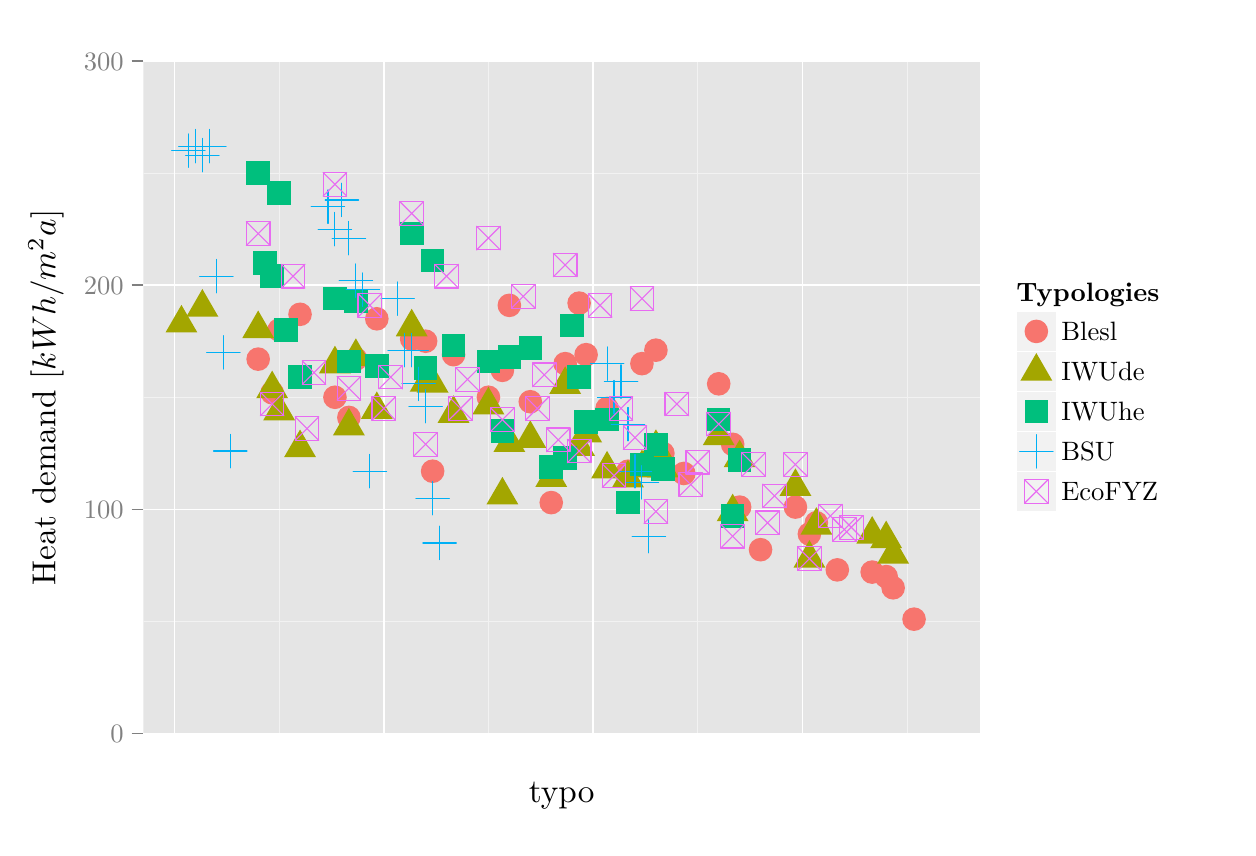
\begin{tikzpicture}[x=1pt,y=1pt]
\definecolor[named]{fillColor}{rgb}{0.00,0.00,0.00}
\path[use as bounding box,fill=fillColor,fill opacity=0.00] (0,0) rectangle (433.62,289.08);
\begin{scope}
\path[clip] (  0.00,  0.00) rectangle (433.62,289.08);
\definecolor[named]{drawColor}{rgb}{1.00,1.00,1.00}
\definecolor[named]{fillColor}{rgb}{1.00,1.00,1.00}

\path[draw=drawColor,line width= 0.6pt,line join=round,line cap=round,fill=fillColor] ( -0.00,  0.00) rectangle (433.62,289.08);
\end{scope}
\begin{scope}
\path[clip] ( 41.82, 34.03) rectangle (344.12,277.03);
\definecolor[named]{fillColor}{rgb}{0.90,0.90,0.90}

\path[fill=fillColor] ( 41.82, 34.03) rectangle (344.12,277.03);
\definecolor[named]{drawColor}{rgb}{0.95,0.95,0.95}

\path[draw=drawColor,line width= 0.3pt,line join=round] ( 41.82, 74.53) --
	(344.12, 74.53);

\path[draw=drawColor,line width= 0.3pt,line join=round] ( 41.82,155.53) --
	(344.12,155.53);

\path[draw=drawColor,line width= 0.3pt,line join=round] ( 41.82,236.53) --
	(344.12,236.53);

\path[draw=drawColor,line width= 0.3pt,line join=round] ( 90.86, 34.03) --
	( 90.86,277.03);

\path[draw=drawColor,line width= 0.3pt,line join=round] (166.50, 34.03) --
	(166.50,277.03);

\path[draw=drawColor,line width= 0.3pt,line join=round] (242.13, 34.03) --
	(242.13,277.03);

\path[draw=drawColor,line width= 0.3pt,line join=round] (317.77, 34.03) --
	(317.77,277.03);
\definecolor[named]{drawColor}{rgb}{1.00,1.00,1.00}

\path[draw=drawColor,line width= 0.6pt,line join=round] ( 41.82, 34.03) --
	(344.12, 34.03);

\path[draw=drawColor,line width= 0.6pt,line join=round] ( 41.82,115.03) --
	(344.12,115.03);

\path[draw=drawColor,line width= 0.6pt,line join=round] ( 41.82,196.03) --
	(344.12,196.03);

\path[draw=drawColor,line width= 0.6pt,line join=round] ( 41.82,277.03) --
	(344.12,277.03);

\path[draw=drawColor,line width= 0.6pt,line join=round] ( 53.04, 34.03) --
	( 53.04,277.03);

\path[draw=drawColor,line width= 0.6pt,line join=round] (128.68, 34.03) --
	(128.68,277.03);

\path[draw=drawColor,line width= 0.6pt,line join=round] (204.31, 34.03) --
	(204.31,277.03);

\path[draw=drawColor,line width= 0.6pt,line join=round] (279.95, 34.03) --
	(279.95,277.03);
\definecolor[named]{fillColor}{rgb}{0.97,0.46,0.43}

\path[fill=fillColor] ( 83.29,169.30) circle (  4.27);

\path[fill=fillColor] ( 88.34,157.15) circle (  4.27);

\path[fill=fillColor] ( 90.86,179.83) circle (  4.27);

\path[fill=fillColor] ( 98.42,185.50) circle (  4.27);

\path[fill=fillColor] (111.03,155.53) circle (  4.27);

\path[fill=fillColor] (116.07,148.24) circle (  4.27);

\path[fill=fillColor] (118.59,169.30) circle (  4.27);

\path[fill=fillColor] (126.16,183.88) circle (  4.27);

\path[fill=fillColor] (138.76,176.59) circle (  4.27);

\path[fill=fillColor] (143.80,175.78) circle (  4.27);

\path[fill=fillColor] (146.33,128.80) circle (  4.27);

\path[fill=fillColor] (153.89,170.92) circle (  4.27);

\path[fill=fillColor] (166.50,155.53) circle (  4.27);

\path[fill=fillColor] (171.54,165.25) circle (  4.27);

\path[fill=fillColor] (174.06,188.74) circle (  4.27);

\path[fill=fillColor] (181.62,153.91) circle (  4.27);

\path[fill=fillColor] (189.19,117.46) circle (  4.27);

\path[fill=fillColor] (194.23,167.68) circle (  4.27);

\path[fill=fillColor] (199.27,189.55) circle (  4.27);

\path[fill=fillColor] (201.79,170.92) circle (  4.27);

\path[fill=fillColor] (209.36,151.48) circle (  4.27);

\path[fill=fillColor] (216.92,128.80) circle (  4.27);

\path[fill=fillColor] (221.96,167.68) circle (  4.27);

\path[fill=fillColor] (227.01,172.54) circle (  4.27);

\path[fill=fillColor] (229.53,135.28) circle (  4.27);

\path[fill=fillColor] (237.09,127.99) circle (  4.27);

\path[fill=fillColor] (249.70,160.39) circle (  4.27);

\path[fill=fillColor] (254.74,138.52) circle (  4.27);

\path[fill=fillColor] (257.26,115.84) circle (  4.27);

\path[fill=fillColor] (264.82,100.45) circle (  4.27);

\path[fill=fillColor] (277.43,115.84) circle (  4.27);

\path[fill=fillColor] (282.47,106.12) circle (  4.27);

\path[fill=fillColor] (284.99,110.17) circle (  4.27);

\path[fill=fillColor] (292.56, 93.16) circle (  4.27);

\path[fill=fillColor] (305.16, 92.35) circle (  4.27);

\path[fill=fillColor] (310.21, 90.73) circle (  4.27);

\path[fill=fillColor] (312.73, 86.68) circle (  4.27);

\path[fill=fillColor] (320.29, 75.34) circle (  4.27);
\definecolor[named]{fillColor}{rgb}{0.64,0.65,0.00}

\path[fill=fillColor] ( 55.56,188.90) --
	( 61.31,178.95) --
	( 49.81,178.95) --
	cycle;

\path[fill=fillColor] ( 63.12,194.65) --
	( 68.87,184.70) --
	( 57.38,184.70) --
	cycle;

\path[fill=fillColor] ( 83.29,186.88) --
	( 89.04,176.92) --
	( 77.55,176.92) --
	cycle;

\path[fill=fillColor] ( 88.34,165.17) --
	( 94.08,155.21) --
	( 82.59,155.21) --
	cycle;

\path[fill=fillColor] ( 90.86,157.15) --
	( 96.61,147.19) --
	( 85.11,147.19) --
	cycle;

\path[fill=fillColor] ( 98.42,143.87) --
	(104.17,133.91) --
	( 92.67,133.91) --
	cycle;

\path[fill=fillColor] (111.03,174.16) --
	(116.78,164.20) --
	(105.28,164.20) --
	cycle;

\path[fill=fillColor] (116.07,151.72) --
	(121.82,141.77) --
	(110.32,141.77) --
	cycle;

\path[fill=fillColor] (118.59,176.83) --
	(124.34,166.88) --
	(112.84,166.88) --
	cycle;

\path[fill=fillColor] (126.16,157.64) --
	(131.90,147.68) --
	(120.41,147.68) --
	cycle;

\path[fill=fillColor] (138.76,187.52) --
	(144.51,177.57) --
	(133.01,177.57) --
	cycle;

\path[fill=fillColor] (143.80,167.52) --
	(149.55,157.56) --
	(138.06,157.56) --
	cycle;

\path[fill=fillColor] (146.33,167.19) --
	(152.07,157.24) --
	(140.58,157.24) --
	cycle;

\path[fill=fillColor] (153.89,156.26) --
	(159.64,146.30) --
	(148.14,146.30) --
	cycle;

\path[fill=fillColor] (166.50,159.34) --
	(172.24,149.38) --
	(160.75,149.38) --
	cycle;

\path[fill=fillColor] (171.54,126.77) --
	(177.29,116.82) --
	(165.79,116.82) --
	cycle;

\path[fill=fillColor] (174.06,145.73) --
	(179.81,135.77) --
	(168.31,135.77) --
	cycle;

\path[fill=fillColor] (181.62,147.19) --
	(187.37,137.23) --
	(175.88,137.23) --
	cycle;

\path[fill=fillColor] (189.19,133.09) --
	(194.93,123.14) --
	(183.44,123.14) --
	cycle;

\path[fill=fillColor] (194.23,166.71) --
	(199.98,156.75) --
	(188.48,156.75) --
	cycle;

\path[fill=fillColor] (199.27,144.27) --
	(205.02,134.32) --
	(193.52,134.32) --
	cycle;

\path[fill=fillColor] (201.79,149.21) --
	(207.54,139.26) --
	(196.05,139.26) --
	cycle;

\path[fill=fillColor] (209.36,136.17) --
	(215.10,126.22) --
	(203.61,126.22) --
	cycle;

\path[fill=fillColor] (216.92,132.93) --
	(222.67,122.98) --
	(211.17,122.98) --
	cycle;

\path[fill=fillColor] (221.96,136.58) --
	(227.71,126.62) --
	(216.22,126.62) --
	cycle;

\path[fill=fillColor] (227.01,143.95) --
	(232.75,133.99) --
	(221.26,133.99) --
	cycle;

\path[fill=fillColor] (229.53,136.49) --
	(235.27,126.54) --
	(223.78,126.54) --
	cycle;

\path[fill=fillColor] (249.70,148.16) --
	(255.44,138.20) --
	(243.95,138.20) --
	cycle;

\path[fill=fillColor] (254.74,120.70) --
	(260.49,110.74) --
	(248.99,110.74) --
	cycle;

\path[fill=fillColor] (257.26,140.22) --
	(263.01,130.27) --
	(251.51,130.27) --
	cycle;

\path[fill=fillColor] (277.43,129.85) --
	(283.18,119.90) --
	(271.68,119.90) --
	cycle;

\path[fill=fillColor] (282.47,103.93) --
	(288.22, 93.98) --
	(276.73, 93.98) --
	cycle;

\path[fill=fillColor] (284.99,115.84) --
	(290.74,105.88) --
	(279.25,105.88) --
	cycle;

\path[fill=fillColor] (305.16,112.60) --
	(310.91,102.64) --
	(299.42,102.64) --
	cycle;

\path[fill=fillColor] (310.21,110.98) --
	(315.95,101.02) --
	(304.46,101.02) --
	cycle;

\path[fill=fillColor] (312.73,105.39) --
	(318.48, 95.44) --
	(306.98, 95.44) --
	cycle;
\definecolor[named]{fillColor}{rgb}{0.00,0.75,0.49}

\path[fill=fillColor] ( 79.03,232.27) --
	( 87.56,232.27) --
	( 87.56,240.80) --
	( 79.03,240.80) --
	cycle;

\path[fill=fillColor] ( 81.55,199.87) --
	( 90.08,199.87) --
	( 90.08,208.40) --
	( 81.55,208.40) --
	cycle;

\path[fill=fillColor] ( 84.07,195.01) --
	( 92.60,195.01) --
	( 92.60,203.54) --
	( 84.07,203.54) --
	cycle;

\path[fill=fillColor] ( 86.59,224.98) --
	( 95.13,224.98) --
	( 95.13,233.51) --
	( 86.59,233.51) --
	cycle;

\path[fill=fillColor] ( 89.11,175.57) --
	( 97.65,175.57) --
	( 97.65,184.10) --
	( 89.11,184.10) --
	cycle;

\path[fill=fillColor] ( 94.15,158.56) --
	(102.69,158.56) --
	(102.69,167.09) --
	( 94.15,167.09) --
	cycle;

\path[fill=fillColor] (106.76,186.91) --
	(115.30,186.91) --
	(115.30,195.44) --
	(106.76,195.44) --
	cycle;

\path[fill=fillColor] (111.80,164.23) --
	(120.34,164.23) --
	(120.34,172.76) --
	(111.80,172.76) --
	cycle;

\path[fill=fillColor] (114.32,186.10) --
	(122.86,186.10) --
	(122.86,194.63) --
	(114.32,194.63) --
	cycle;

\path[fill=fillColor] (121.89,162.61) --
	(130.42,162.61) --
	(130.42,171.14) --
	(121.89,171.14) --
	cycle;

\path[fill=fillColor] (134.49,210.40) --
	(143.03,210.40) --
	(143.03,218.93) --
	(134.49,218.93) --
	cycle;

\path[fill=fillColor] (139.54,161.80) --
	(148.07,161.80) --
	(148.07,170.33) --
	(139.54,170.33) --
	cycle;

\path[fill=fillColor] (142.06,200.68) --
	(150.59,200.68) --
	(150.59,209.21) --
	(142.06,209.21) --
	cycle;

\path[fill=fillColor] (149.62,169.90) --
	(158.16,169.90) --
	(158.16,178.43) --
	(149.62,178.43) --
	cycle;

\path[fill=fillColor] (162.23,164.23) --
	(170.76,164.23) --
	(170.76,172.76) --
	(162.23,172.76) --
	cycle;

\path[fill=fillColor] (167.27,139.12) --
	(175.81,139.12) --
	(175.81,147.65) --
	(167.27,147.65) --
	cycle;

\path[fill=fillColor] (169.79,165.85) --
	(178.33,165.85) --
	(178.33,174.38) --
	(169.79,174.38) --
	cycle;

\path[fill=fillColor] (177.36,169.09) --
	(185.89,169.09) --
	(185.89,177.62) --
	(177.36,177.62) --
	cycle;

\path[fill=fillColor] (184.92,126.16) --
	(193.45,126.16) --
	(193.45,134.69) --
	(184.92,134.69) --
	cycle;

\path[fill=fillColor] (189.96,129.40) --
	(198.50,129.40) --
	(198.50,137.93) --
	(189.96,137.93) --
	cycle;

\path[fill=fillColor] (192.48,177.19) --
	(201.02,177.19) --
	(201.02,185.72) --
	(192.48,185.72) --
	cycle;

\path[fill=fillColor] (195.00,158.56) --
	(203.54,158.56) --
	(203.54,167.09) --
	(195.00,167.09) --
	cycle;

\path[fill=fillColor] (197.53,142.36) --
	(206.06,142.36) --
	(206.06,150.89) --
	(197.53,150.89) --
	cycle;

\path[fill=fillColor] (205.09,143.17) --
	(213.62,143.17) --
	(213.62,151.70) --
	(205.09,151.70) --
	cycle;

\path[fill=fillColor] (212.65,113.20) --
	(221.19,113.20) --
	(221.19,121.73) --
	(212.65,121.73) --
	cycle;

\path[fill=fillColor] (217.70,126.97) --
	(226.23,126.97) --
	(226.23,135.50) --
	(217.70,135.50) --
	cycle;

\path[fill=fillColor] (222.74,134.26) --
	(231.27,134.26) --
	(231.27,142.79) --
	(222.74,142.79) --
	cycle;

\path[fill=fillColor] (225.26,125.35) --
	(233.79,125.35) --
	(233.79,133.88) --
	(225.26,133.88) --
	cycle;

\path[fill=fillColor] (245.43,143.17) --
	(253.96,143.17) --
	(253.96,151.70) --
	(245.43,151.70) --
	cycle;

\path[fill=fillColor] (250.47,108.34) --
	(259.01,108.34) --
	(259.01,116.87) --
	(250.47,116.87) --
	cycle;

\path[fill=fillColor] (252.99,128.59) --
	(261.53,128.59) --
	(261.53,137.12) --
	(252.99,137.12) --
	cycle;
\definecolor[named]{drawColor}{rgb}{0.00,0.69,0.96}

\path[draw=drawColor,line width= 0.4pt,line join=round,line cap=round] ( 52.05,244.63) -- ( 64.12,244.63);

\path[draw=drawColor,line width= 0.4pt,line join=round,line cap=round] ( 58.08,238.60) -- ( 58.08,250.67);

\path[draw=drawColor,line width= 0.4pt,line join=round,line cap=round] ( 54.57,246.25) -- ( 66.64,246.25);

\path[draw=drawColor,line width= 0.4pt,line join=round,line cap=round] ( 60.60,240.22) -- ( 60.60,252.29);

\path[draw=drawColor,line width= 0.4pt,line join=round,line cap=round] ( 57.09,243.01) -- ( 69.16,243.01);

\path[draw=drawColor,line width= 0.4pt,line join=round,line cap=round] ( 63.12,236.98) -- ( 63.12,249.05);

\path[draw=drawColor,line width= 0.4pt,line join=round,line cap=round] ( 59.61,246.25) -- ( 71.68,246.25);

\path[draw=drawColor,line width= 0.4pt,line join=round,line cap=round] ( 65.65,240.22) -- ( 65.65,252.29);

\path[draw=drawColor,line width= 0.4pt,line join=round,line cap=round] ( 62.13,199.27) -- ( 74.20,199.27);

\path[draw=drawColor,line width= 0.4pt,line join=round,line cap=round] ( 68.17,193.24) -- ( 68.17,205.31);

\path[draw=drawColor,line width= 0.4pt,line join=round,line cap=round] ( 64.65,171.73) -- ( 76.72,171.73);

\path[draw=drawColor,line width= 0.4pt,line join=round,line cap=round] ( 70.69,165.70) -- ( 70.69,177.77);

\path[draw=drawColor,line width= 0.4pt,line join=round,line cap=round] ( 67.17,136.09) -- ( 79.24,136.09);

\path[draw=drawColor,line width= 0.4pt,line join=round,line cap=round] ( 73.21,130.06) -- ( 73.21,142.13);

\path[draw=drawColor,line width= 0.4pt,line join=round,line cap=round] (102.47,224.38) -- (114.54,224.38);

\path[draw=drawColor,line width= 0.4pt,line join=round,line cap=round] (108.51,218.35) -- (108.51,230.42);

\path[draw=drawColor,line width= 0.4pt,line join=round,line cap=round] (104.99,216.28) -- (117.06,216.28);

\path[draw=drawColor,line width= 0.4pt,line join=round,line cap=round] (111.03,210.25) -- (111.03,222.32);

\path[draw=drawColor,line width= 0.4pt,line join=round,line cap=round] (107.51,226.81) -- (119.58,226.81);

\path[draw=drawColor,line width= 0.4pt,line join=round,line cap=round] (113.55,220.78) -- (113.55,232.85);

\path[draw=drawColor,line width= 0.4pt,line join=round,line cap=round] (110.03,213.04) -- (122.11,213.04);

\path[draw=drawColor,line width= 0.4pt,line join=round,line cap=round] (116.07,207.01) -- (116.07,219.08);

\path[draw=drawColor,line width= 0.4pt,line join=round,line cap=round] (112.56,197.65) -- (124.63,197.65);

\path[draw=drawColor,line width= 0.4pt,line join=round,line cap=round] (118.59,191.62) -- (118.59,203.69);

\path[draw=drawColor,line width= 0.4pt,line join=round,line cap=round] (115.08,194.41) -- (127.15,194.41);

\path[draw=drawColor,line width= 0.4pt,line join=round,line cap=round] (121.11,188.38) -- (121.11,200.45);

\path[draw=drawColor,line width= 0.4pt,line join=round,line cap=round] (117.60,128.80) -- (129.67,128.80);

\path[draw=drawColor,line width= 0.4pt,line join=round,line cap=round] (123.63,122.77) -- (123.63,134.84);

\path[draw=drawColor,line width= 0.4pt,line join=round,line cap=round] (127.68,191.17) -- (139.75,191.17);

\path[draw=drawColor,line width= 0.4pt,line join=round,line cap=round] (133.72,185.14) -- (133.72,197.21);

\path[draw=drawColor,line width= 0.4pt,line join=round,line cap=round] (130.20,172.54) -- (142.28,172.54);

\path[draw=drawColor,line width= 0.4pt,line join=round,line cap=round] (136.24,166.51) -- (136.24,178.58);

\path[draw=drawColor,line width= 0.4pt,line join=round,line cap=round] (132.73,172.54) -- (144.80,172.54);

\path[draw=drawColor,line width= 0.4pt,line join=round,line cap=round] (138.76,166.51) -- (138.76,178.58);

\path[draw=drawColor,line width= 0.4pt,line join=round,line cap=round] (135.25,160.39) -- (147.32,160.39);

\path[draw=drawColor,line width= 0.4pt,line join=round,line cap=round] (141.28,154.36) -- (141.28,166.43);

\path[draw=drawColor,line width= 0.4pt,line join=round,line cap=round] (137.77,152.29) -- (149.84,152.29);

\path[draw=drawColor,line width= 0.4pt,line join=round,line cap=round] (143.80,146.26) -- (143.80,158.33);

\path[draw=drawColor,line width= 0.4pt,line join=round,line cap=round] (140.29,119.08) -- (152.36,119.08);

\path[draw=drawColor,line width= 0.4pt,line join=round,line cap=round] (146.33,113.05) -- (146.33,125.12);

\path[draw=drawColor,line width= 0.4pt,line join=round,line cap=round] (142.81,102.88) -- (154.88,102.88);

\path[draw=drawColor,line width= 0.4pt,line join=round,line cap=round] (148.85, 96.85) -- (148.85,108.92);

\path[draw=drawColor,line width= 0.4pt,line join=round,line cap=round] (203.32,167.68) -- (215.39,167.68);

\path[draw=drawColor,line width= 0.4pt,line join=round,line cap=round] (209.36,161.65) -- (209.36,173.72);

\path[draw=drawColor,line width= 0.4pt,line join=round,line cap=round] (205.84,155.53) -- (217.91,155.53);

\path[draw=drawColor,line width= 0.4pt,line join=round,line cap=round] (211.88,149.50) -- (211.88,161.57);

\path[draw=drawColor,line width= 0.4pt,line join=round,line cap=round] (208.36,161.20) -- (220.44,161.20);

\path[draw=drawColor,line width= 0.4pt,line join=round,line cap=round] (214.40,155.17) -- (214.40,167.24);

\path[draw=drawColor,line width= 0.4pt,line join=round,line cap=round] (210.88,145.81) -- (222.96,145.81);

\path[draw=drawColor,line width= 0.4pt,line join=round,line cap=round] (216.92,139.78) -- (216.92,151.85);

\path[draw=drawColor,line width= 0.4pt,line join=round,line cap=round] (213.41,128.80) -- (225.48,128.80);

\path[draw=drawColor,line width= 0.4pt,line join=round,line cap=round] (219.44,122.77) -- (219.44,134.84);

\path[draw=drawColor,line width= 0.4pt,line join=round,line cap=round] (215.93,124.75) -- (228.00,124.75);

\path[draw=drawColor,line width= 0.4pt,line join=round,line cap=round] (221.96,118.72) -- (221.96,130.79);

\path[draw=drawColor,line width= 0.4pt,line join=round,line cap=round] (218.45,105.31) -- (230.52,105.31);

\path[draw=drawColor,line width= 0.4pt,line join=round,line cap=round] (224.48, 99.28) -- (224.48,111.35);
\definecolor[named]{drawColor}{rgb}{0.91,0.42,0.95}

\path[draw=drawColor,line width= 0.4pt,line join=round,line cap=round] ( 79.03,210.40) rectangle ( 87.56,218.93);

\path[draw=drawColor,line width= 0.4pt,line join=round,line cap=round] ( 79.03,210.40) -- ( 87.56,218.93);

\path[draw=drawColor,line width= 0.4pt,line join=round,line cap=round] ( 79.03,218.93) -- ( 87.56,210.40);

\path[draw=drawColor,line width= 0.4pt,line join=round,line cap=round] ( 84.07,148.84) rectangle ( 92.60,157.37);

\path[draw=drawColor,line width= 0.4pt,line join=round,line cap=round] ( 84.07,148.84) -- ( 92.60,157.37);

\path[draw=drawColor,line width= 0.4pt,line join=round,line cap=round] ( 84.07,157.37) -- ( 92.60,148.84);

\path[draw=drawColor,line width= 0.4pt,line join=round,line cap=round] ( 91.63,195.01) rectangle (100.17,203.54);

\path[draw=drawColor,line width= 0.4pt,line join=round,line cap=round] ( 91.63,195.01) -- (100.17,203.54);

\path[draw=drawColor,line width= 0.4pt,line join=round,line cap=round] ( 91.63,203.54) -- (100.17,195.01);

\path[draw=drawColor,line width= 0.4pt,line join=round,line cap=round] ( 96.67,139.93) rectangle (105.21,148.46);

\path[draw=drawColor,line width= 0.4pt,line join=round,line cap=round] ( 96.67,139.93) -- (105.21,148.46);

\path[draw=drawColor,line width= 0.4pt,line join=round,line cap=round] ( 96.67,148.46) -- (105.21,139.93);

\path[draw=drawColor,line width= 0.4pt,line join=round,line cap=round] ( 99.20,160.18) rectangle (107.73,168.71);

\path[draw=drawColor,line width= 0.4pt,line join=round,line cap=round] ( 99.20,160.18) -- (107.73,168.71);

\path[draw=drawColor,line width= 0.4pt,line join=round,line cap=round] ( 99.20,168.71) -- (107.73,160.18);

\path[draw=drawColor,line width= 0.4pt,line join=round,line cap=round] (106.76,228.22) rectangle (115.30,236.75);

\path[draw=drawColor,line width= 0.4pt,line join=round,line cap=round] (106.76,228.22) -- (115.30,236.75);

\path[draw=drawColor,line width= 0.4pt,line join=round,line cap=round] (106.76,236.75) -- (115.30,228.22);

\path[draw=drawColor,line width= 0.4pt,line join=round,line cap=round] (111.80,154.51) rectangle (120.34,163.04);

\path[draw=drawColor,line width= 0.4pt,line join=round,line cap=round] (111.80,154.51) -- (120.34,163.04);

\path[draw=drawColor,line width= 0.4pt,line join=round,line cap=round] (111.80,163.04) -- (120.34,154.51);

\path[draw=drawColor,line width= 0.4pt,line join=round,line cap=round] (119.37,184.48) rectangle (127.90,193.01);

\path[draw=drawColor,line width= 0.4pt,line join=round,line cap=round] (119.37,184.48) -- (127.90,193.01);

\path[draw=drawColor,line width= 0.4pt,line join=round,line cap=round] (119.37,193.01) -- (127.90,184.48);

\path[draw=drawColor,line width= 0.4pt,line join=round,line cap=round] (124.41,147.22) rectangle (132.94,155.75);

\path[draw=drawColor,line width= 0.4pt,line join=round,line cap=round] (124.41,147.22) -- (132.94,155.75);

\path[draw=drawColor,line width= 0.4pt,line join=round,line cap=round] (124.41,155.75) -- (132.94,147.22);

\path[draw=drawColor,line width= 0.4pt,line join=round,line cap=round] (126.93,158.56) rectangle (135.47,167.09);

\path[draw=drawColor,line width= 0.4pt,line join=round,line cap=round] (126.93,158.56) -- (135.47,167.09);

\path[draw=drawColor,line width= 0.4pt,line join=round,line cap=round] (126.93,167.09) -- (135.47,158.56);

\path[draw=drawColor,line width= 0.4pt,line join=round,line cap=round] (134.49,217.69) rectangle (143.03,226.22);

\path[draw=drawColor,line width= 0.4pt,line join=round,line cap=round] (134.49,217.69) -- (143.03,226.22);

\path[draw=drawColor,line width= 0.4pt,line join=round,line cap=round] (134.49,226.22) -- (143.03,217.69);

\path[draw=drawColor,line width= 0.4pt,line join=round,line cap=round] (139.54,134.26) rectangle (148.07,142.79);

\path[draw=drawColor,line width= 0.4pt,line join=round,line cap=round] (139.54,134.26) -- (148.07,142.79);

\path[draw=drawColor,line width= 0.4pt,line join=round,line cap=round] (139.54,142.79) -- (148.07,134.26);

\path[draw=drawColor,line width= 0.4pt,line join=round,line cap=round] (147.10,195.01) rectangle (155.64,203.54);

\path[draw=drawColor,line width= 0.4pt,line join=round,line cap=round] (147.10,195.01) -- (155.64,203.54);

\path[draw=drawColor,line width= 0.4pt,line join=round,line cap=round] (147.10,203.54) -- (155.64,195.01);

\path[draw=drawColor,line width= 0.4pt,line join=round,line cap=round] (152.14,147.22) rectangle (160.68,155.75);

\path[draw=drawColor,line width= 0.4pt,line join=round,line cap=round] (152.14,147.22) -- (160.68,155.75);

\path[draw=drawColor,line width= 0.4pt,line join=round,line cap=round] (152.14,155.75) -- (160.68,147.22);

\path[draw=drawColor,line width= 0.4pt,line join=round,line cap=round] (154.66,157.75) rectangle (163.20,166.28);

\path[draw=drawColor,line width= 0.4pt,line join=round,line cap=round] (154.66,157.75) -- (163.20,166.28);

\path[draw=drawColor,line width= 0.4pt,line join=round,line cap=round] (154.66,166.28) -- (163.20,157.75);

\path[draw=drawColor,line width= 0.4pt,line join=round,line cap=round] (162.23,208.78) rectangle (170.76,217.31);

\path[draw=drawColor,line width= 0.4pt,line join=round,line cap=round] (162.23,208.78) -- (170.76,217.31);

\path[draw=drawColor,line width= 0.4pt,line join=round,line cap=round] (162.23,217.31) -- (170.76,208.78);

\path[draw=drawColor,line width= 0.4pt,line join=round,line cap=round] (167.27,143.17) rectangle (175.81,151.70);

\path[draw=drawColor,line width= 0.4pt,line join=round,line cap=round] (167.27,143.17) -- (175.81,151.70);

\path[draw=drawColor,line width= 0.4pt,line join=round,line cap=round] (167.27,151.70) -- (175.81,143.17);

\path[draw=drawColor,line width= 0.4pt,line join=round,line cap=round] (174.83,187.72) rectangle (183.37,196.25);

\path[draw=drawColor,line width= 0.4pt,line join=round,line cap=round] (174.83,187.72) -- (183.37,196.25);

\path[draw=drawColor,line width= 0.4pt,line join=round,line cap=round] (174.83,196.25) -- (183.37,187.72);

\path[draw=drawColor,line width= 0.4pt,line join=round,line cap=round] (179.88,147.22) rectangle (188.41,155.75);

\path[draw=drawColor,line width= 0.4pt,line join=round,line cap=round] (179.88,147.22) -- (188.41,155.75);

\path[draw=drawColor,line width= 0.4pt,line join=round,line cap=round] (179.88,155.75) -- (188.41,147.22);

\path[draw=drawColor,line width= 0.4pt,line join=round,line cap=round] (182.40,159.37) rectangle (190.93,167.90);

\path[draw=drawColor,line width= 0.4pt,line join=round,line cap=round] (182.40,159.37) -- (190.93,167.90);

\path[draw=drawColor,line width= 0.4pt,line join=round,line cap=round] (182.40,167.90) -- (190.93,159.37);

\path[draw=drawColor,line width= 0.4pt,line join=round,line cap=round] (187.44,135.88) rectangle (195.98,144.41);

\path[draw=drawColor,line width= 0.4pt,line join=round,line cap=round] (187.44,135.88) -- (195.98,144.41);

\path[draw=drawColor,line width= 0.4pt,line join=round,line cap=round] (187.44,144.41) -- (195.98,135.88);

\path[draw=drawColor,line width= 0.4pt,line join=round,line cap=round] (189.96,199.06) rectangle (198.50,207.59);

\path[draw=drawColor,line width= 0.4pt,line join=round,line cap=round] (189.96,199.06) -- (198.50,207.59);

\path[draw=drawColor,line width= 0.4pt,line join=round,line cap=round] (189.96,207.59) -- (198.50,199.06);

\path[draw=drawColor,line width= 0.4pt,line join=round,line cap=round] (195.00,131.83) rectangle (203.54,140.36);

\path[draw=drawColor,line width= 0.4pt,line join=round,line cap=round] (195.00,131.83) -- (203.54,140.36);

\path[draw=drawColor,line width= 0.4pt,line join=round,line cap=round] (195.00,140.36) -- (203.54,131.83);

\path[draw=drawColor,line width= 0.4pt,line join=round,line cap=round] (202.57,184.48) rectangle (211.10,193.01);

\path[draw=drawColor,line width= 0.4pt,line join=round,line cap=round] (202.57,184.48) -- (211.10,193.01);

\path[draw=drawColor,line width= 0.4pt,line join=round,line cap=round] (202.57,193.01) -- (211.10,184.48);

\path[draw=drawColor,line width= 0.4pt,line join=round,line cap=round] (207.61,122.92) rectangle (216.15,131.45);

\path[draw=drawColor,line width= 0.4pt,line join=round,line cap=round] (207.61,122.92) -- (216.15,131.45);

\path[draw=drawColor,line width= 0.4pt,line join=round,line cap=round] (207.61,131.45) -- (216.15,122.92);

\path[draw=drawColor,line width= 0.4pt,line join=round,line cap=round] (210.13,147.22) rectangle (218.67,155.75);

\path[draw=drawColor,line width= 0.4pt,line join=round,line cap=round] (210.13,147.22) -- (218.67,155.75);

\path[draw=drawColor,line width= 0.4pt,line join=round,line cap=round] (210.13,155.75) -- (218.67,147.22);

\path[draw=drawColor,line width= 0.4pt,line join=round,line cap=round] (215.17,136.69) rectangle (223.71,145.22);

\path[draw=drawColor,line width= 0.4pt,line join=round,line cap=round] (215.17,136.69) -- (223.71,145.22);

\path[draw=drawColor,line width= 0.4pt,line join=round,line cap=round] (215.17,145.22) -- (223.71,136.69);

\path[draw=drawColor,line width= 0.4pt,line join=round,line cap=round] (217.70,186.91) rectangle (226.23,195.44);

\path[draw=drawColor,line width= 0.4pt,line join=round,line cap=round] (217.70,186.91) -- (226.23,195.44);

\path[draw=drawColor,line width= 0.4pt,line join=round,line cap=round] (217.70,195.44) -- (226.23,186.91);

\path[draw=drawColor,line width= 0.4pt,line join=round,line cap=round] (222.74,109.96) rectangle (231.27,118.49);

\path[draw=drawColor,line width= 0.4pt,line join=round,line cap=round] (222.74,109.96) -- (231.27,118.49);

\path[draw=drawColor,line width= 0.4pt,line join=round,line cap=round] (222.74,118.49) -- (231.27,109.96);

\path[draw=drawColor,line width= 0.4pt,line join=round,line cap=round] (230.30,148.84) rectangle (238.84,157.37);

\path[draw=drawColor,line width= 0.4pt,line join=round,line cap=round] (230.30,148.84) -- (238.84,157.37);

\path[draw=drawColor,line width= 0.4pt,line join=round,line cap=round] (230.30,157.37) -- (238.84,148.84);

\path[draw=drawColor,line width= 0.4pt,line join=round,line cap=round] (235.34,119.68) rectangle (243.88,128.21);

\path[draw=drawColor,line width= 0.4pt,line join=round,line cap=round] (235.34,119.68) -- (243.88,128.21);

\path[draw=drawColor,line width= 0.4pt,line join=round,line cap=round] (235.34,128.21) -- (243.88,119.68);

\path[draw=drawColor,line width= 0.4pt,line join=round,line cap=round] (237.87,127.78) rectangle (246.40,136.31);

\path[draw=drawColor,line width= 0.4pt,line join=round,line cap=round] (237.87,127.78) -- (246.40,136.31);

\path[draw=drawColor,line width= 0.4pt,line join=round,line cap=round] (237.87,136.31) -- (246.40,127.78);

\path[draw=drawColor,line width= 0.4pt,line join=round,line cap=round] (245.43,141.55) rectangle (253.96,150.08);

\path[draw=drawColor,line width= 0.4pt,line join=round,line cap=round] (245.43,141.55) -- (253.96,150.08);

\path[draw=drawColor,line width= 0.4pt,line join=round,line cap=round] (245.43,150.08) -- (253.96,141.55);

\path[draw=drawColor,line width= 0.4pt,line join=round,line cap=round] (250.47,101.05) rectangle (259.01,109.58);

\path[draw=drawColor,line width= 0.4pt,line join=round,line cap=round] (250.47,101.05) -- (259.01,109.58);

\path[draw=drawColor,line width= 0.4pt,line join=round,line cap=round] (250.47,109.58) -- (259.01,101.05);

\path[draw=drawColor,line width= 0.4pt,line join=round,line cap=round] (258.04,126.97) rectangle (266.57,135.50);

\path[draw=drawColor,line width= 0.4pt,line join=round,line cap=round] (258.04,126.97) -- (266.57,135.50);

\path[draw=drawColor,line width= 0.4pt,line join=round,line cap=round] (258.04,135.50) -- (266.57,126.97);

\path[draw=drawColor,line width= 0.4pt,line join=round,line cap=round] (263.08,105.91) rectangle (271.61,114.44);

\path[draw=drawColor,line width= 0.4pt,line join=round,line cap=round] (263.08,105.91) -- (271.61,114.44);

\path[draw=drawColor,line width= 0.4pt,line join=round,line cap=round] (263.08,114.44) -- (271.61,105.91);

\path[draw=drawColor,line width= 0.4pt,line join=round,line cap=round] (265.60,115.63) rectangle (274.13,124.16);

\path[draw=drawColor,line width= 0.4pt,line join=round,line cap=round] (265.60,115.63) -- (274.13,124.16);

\path[draw=drawColor,line width= 0.4pt,line join=round,line cap=round] (265.60,124.16) -- (274.13,115.63);

\path[draw=drawColor,line width= 0.4pt,line join=round,line cap=round] (273.16,126.97) rectangle (281.70,135.50);

\path[draw=drawColor,line width= 0.4pt,line join=round,line cap=round] (273.16,126.97) -- (281.70,135.50);

\path[draw=drawColor,line width= 0.4pt,line join=round,line cap=round] (273.16,135.50) -- (281.70,126.97);

\path[draw=drawColor,line width= 0.4pt,line join=round,line cap=round] (278.21, 92.95) rectangle (286.74,101.48);

\path[draw=drawColor,line width= 0.4pt,line join=round,line cap=round] (278.21, 92.95) -- (286.74,101.48);

\path[draw=drawColor,line width= 0.4pt,line join=round,line cap=round] (278.21,101.48) -- (286.74, 92.95);

\path[draw=drawColor,line width= 0.4pt,line join=round,line cap=round] (285.77,108.34) rectangle (294.30,116.87);

\path[draw=drawColor,line width= 0.4pt,line join=round,line cap=round] (285.77,108.34) -- (294.30,116.87);

\path[draw=drawColor,line width= 0.4pt,line join=round,line cap=round] (285.77,116.87) -- (294.30,108.34);

\path[draw=drawColor,line width= 0.4pt,line join=round,line cap=round] (290.81,103.48) rectangle (299.35,112.01);

\path[draw=drawColor,line width= 0.4pt,line join=round,line cap=round] (290.81,103.48) -- (299.35,112.01);

\path[draw=drawColor,line width= 0.4pt,line join=round,line cap=round] (290.81,112.01) -- (299.35,103.48);

\path[draw=drawColor,line width= 0.4pt,line join=round,line cap=round] (293.33,104.29) rectangle (301.87,112.82);

\path[draw=drawColor,line width= 0.4pt,line join=round,line cap=round] (293.33,104.29) -- (301.87,112.82);

\path[draw=drawColor,line width= 0.4pt,line join=round,line cap=round] (293.33,112.82) -- (301.87,104.29);
\end{scope}
\begin{scope}
\path[clip] (  0.00,  0.00) rectangle (433.62,289.08);
\definecolor[named]{drawColor}{rgb}{0.50,0.50,0.50}

\node[text=drawColor,anchor=base east,inner sep=0pt, outer sep=0pt, scale=  0.96] at ( 34.71, 30.73) {0};

\node[text=drawColor,anchor=base east,inner sep=0pt, outer sep=0pt, scale=  0.96] at ( 34.71,111.73) {100};

\node[text=drawColor,anchor=base east,inner sep=0pt, outer sep=0pt, scale=  0.96] at ( 34.71,192.73) {200};

\node[text=drawColor,anchor=base east,inner sep=0pt, outer sep=0pt, scale=  0.96] at ( 34.71,273.73) {300};
\end{scope}
\begin{scope}
\path[clip] (  0.00,  0.00) rectangle (433.62,289.08);
\definecolor[named]{drawColor}{rgb}{0.50,0.50,0.50}

\path[draw=drawColor,line width= 0.6pt,line join=round] ( 37.55, 34.03) --
	( 41.82, 34.03);

\path[draw=drawColor,line width= 0.6pt,line join=round] ( 37.55,115.03) --
	( 41.82,115.03);

\path[draw=drawColor,line width= 0.6pt,line join=round] ( 37.55,196.03) --
	( 41.82,196.03);

\path[draw=drawColor,line width= 0.6pt,line join=round] ( 37.55,277.03) --
	( 41.82,277.03);
\end{scope}
% \begin{scope}
% \path[clip] (  0.00,  0.00) rectangle (433.62,289.08);
% \definecolor[named]{drawColor}{rgb}{0.50,0.50,0.50}
% 
% \path[draw=drawColor,line width= 0.6pt,line join=round] ( 53.04, 29.77) --
% 	( 53.04, 34.03);
% 
% \path[draw=drawColor,line width= 0.6pt,line join=round] (128.68, 29.77) --
% 	(128.68, 34.03);
% 
% \path[draw=drawColor,line width= 0.6pt,line join=round] (204.31, 29.77) --
% 	(204.31, 34.03);
% 
% \path[draw=drawColor,line width= 0.6pt,line join=round] (279.95, 29.77) --
% 	(279.95, 34.03);
% \end{scope}
% \begin{scope}
% \path[clip] (  0.00,  0.00) rectangle (433.62,289.08);
% \definecolor[named]{drawColor}{rgb}{0.50,0.50,0.50}

% \node[text=drawColor,anchor=base,inner sep=0pt, outer sep=0pt, scale=  0.96] at ( 53.04, 20.31) {0};
% 
% \node[text=drawColor,anchor=base,inner sep=0pt, outer sep=0pt, scale=  0.96] at (128.68, 20.31) {30};
% 
% \node[text=drawColor,anchor=base,inner sep=0pt, outer sep=0pt, scale=  0.96] at (204.31, 20.31) {60};
% 
% \node[text=drawColor,anchor=base,inner sep=0pt, outer sep=0pt, scale=  0.96] at (279.95, 20.31) {90};
% \end{scope}
\begin{scope}
\path[clip] (  0.00,  0.00) rectangle (433.62,289.08);
\definecolor[named]{drawColor}{rgb}{0.00,0.00,0.00}

\node[text=drawColor,anchor=base,inner sep=0pt, outer sep=0pt, scale=  1.20] at (192.97,  9.03) {typo};
\end{scope}
\begin{scope}
\path[clip] (  0.00,  0.00) rectangle (433.62,289.08);
\definecolor[named]{drawColor}{rgb}{0.00,0.00,0.00}

\node[text=drawColor,rotate= 90.00,anchor=base,inner sep=0pt, outer sep=0pt,
scale=  1.20] at ( 10.00,155.53) {Heat demand $[kWh/m^2a]$};
\end{scope}
\begin{scope}
\path[clip] (  0.00,  0.00) rectangle (433.62,289.08);
\definecolor[named]{fillColor}{rgb}{1.00,1.00,1.00}

\path[fill=fillColor] (352.99,110.01) rectangle (412.71,201.06);
\end{scope}
\begin{scope}
\path[clip] (  0.00,  0.00) rectangle (433.62,289.08);
\definecolor[named]{drawColor}{rgb}{0.00,0.00,0.00}

\node[text=drawColor,anchor=base west,inner sep=0pt, outer sep=0pt, scale= 
0.96] at (357.25,190.16) {\bfseries Typologies};
\end{scope}
\begin{scope}
\path[clip] (  0.00,  0.00) rectangle (433.62,289.08);
\definecolor[named]{drawColor}{rgb}{1.00,1.00,1.00}
\definecolor[named]{fillColor}{rgb}{0.95,0.95,0.95}

\path[draw=drawColor,line width= 0.6pt,line join=round,line cap=round,fill=fillColor] (357.25,172.10) rectangle (371.71,186.55);
\end{scope}
\begin{scope}
\path[clip] (  0.00,  0.00) rectangle (433.62,289.08);
\definecolor[named]{fillColor}{rgb}{0.97,0.46,0.43}

\path[fill=fillColor] (364.48,179.32) circle (  4.27);
\end{scope}
\begin{scope}
\path[clip] (  0.00,  0.00) rectangle (433.62,289.08);
\definecolor[named]{drawColor}{rgb}{1.00,1.00,1.00}
\definecolor[named]{fillColor}{rgb}{0.95,0.95,0.95}

\path[draw=drawColor,line width= 0.6pt,line join=round,line cap=round,fill=fillColor] (357.25,157.64) rectangle (371.71,172.10);
\end{scope}
\begin{scope}
\path[clip] (  0.00,  0.00) rectangle (433.62,289.08);
\definecolor[named]{fillColor}{rgb}{0.64,0.65,0.00}

\path[fill=fillColor] (364.48,171.51) --
	(370.23,161.55) --
	(358.73,161.55) --
	cycle;
\end{scope}
\begin{scope}
\path[clip] (  0.00,  0.00) rectangle (433.62,289.08);
\definecolor[named]{drawColor}{rgb}{1.00,1.00,1.00}
\definecolor[named]{fillColor}{rgb}{0.95,0.95,0.95}

\path[draw=drawColor,line width= 0.6pt,line join=round,line cap=round,fill=fillColor] (357.25,143.19) rectangle (371.71,157.64);
\end{scope}
\begin{scope}
\path[clip] (  0.00,  0.00) rectangle (433.62,289.08);
\definecolor[named]{fillColor}{rgb}{0.00,0.75,0.49}

\path[fill=fillColor] (360.21,146.15) --
	(368.75,146.15) --
	(368.75,154.68) --
	(360.21,154.68) --
	cycle;
\end{scope}
\begin{scope}
\path[clip] (  0.00,  0.00) rectangle (433.62,289.08);
\definecolor[named]{drawColor}{rgb}{1.00,1.00,1.00}
\definecolor[named]{fillColor}{rgb}{0.95,0.95,0.95}

\path[draw=drawColor,line width= 0.6pt,line join=round,line cap=round,fill=fillColor] (357.25,128.73) rectangle (371.71,143.19);
\end{scope}
\begin{scope}
\path[clip] (  0.00,  0.00) rectangle (433.62,289.08);
\definecolor[named]{drawColor}{rgb}{0.00,0.69,0.96}

\path[draw=drawColor,line width= 0.4pt,line join=round,line cap=round] (358.44,135.96) -- (370.52,135.96);

\path[draw=drawColor,line width= 0.4pt,line join=round,line cap=round] (364.48,129.93) -- (364.48,142.00);
\end{scope}
\begin{scope}
\path[clip] (  0.00,  0.00) rectangle (433.62,289.08);
\definecolor[named]{drawColor}{rgb}{1.00,1.00,1.00}
\definecolor[named]{fillColor}{rgb}{0.95,0.95,0.95}

\path[draw=drawColor,line width= 0.6pt,line join=round,line cap=round,fill=fillColor] (357.25,114.28) rectangle (371.71,128.73);
\end{scope}
\begin{scope}
\path[clip] (  0.00,  0.00) rectangle (433.62,289.08);
\definecolor[named]{drawColor}{rgb}{0.91,0.42,0.95}

\path[draw=drawColor,line width= 0.4pt,line join=round,line cap=round] (360.21,117.24) rectangle (368.75,125.78);

\path[draw=drawColor,line width= 0.4pt,line join=round,line cap=round] (360.21,117.24) -- (368.75,125.78);

\path[draw=drawColor,line width= 0.4pt,line join=round,line cap=round] (360.21,125.78) -- (368.75,117.24);
\end{scope}
\begin{scope}
\path[clip] (  0.00,  0.00) rectangle (433.62,289.08);
\definecolor[named]{drawColor}{rgb}{0.00,0.00,0.00}

\node[text=drawColor,anchor=base west,inner sep=0pt, outer sep=0pt, scale=  0.96] at (373.51,176.02) {Blesl};
\end{scope}
\begin{scope}
\path[clip] (  0.00,  0.00) rectangle (433.62,289.08);
\definecolor[named]{drawColor}{rgb}{0.00,0.00,0.00}

\node[text=drawColor,anchor=base west,inner sep=0pt, outer sep=0pt, scale=  0.96] at (373.51,161.56) {IWUde};
\end{scope}
\begin{scope}
\path[clip] (  0.00,  0.00) rectangle (433.62,289.08);
\definecolor[named]{drawColor}{rgb}{0.00,0.00,0.00}

\node[text=drawColor,anchor=base west,inner sep=0pt, outer sep=0pt, scale=  0.96] at (373.51,147.11) {IWUhe};
\end{scope}
\begin{scope}
\path[clip] (  0.00,  0.00) rectangle (433.62,289.08);
\definecolor[named]{drawColor}{rgb}{0.00,0.00,0.00}

\node[text=drawColor,anchor=base west,inner sep=0pt, outer sep=0pt, scale=  0.96] at (373.51,132.66) {BSU};
\end{scope}
\begin{scope}
\path[clip] (  0.00,  0.00) rectangle (433.62,289.08);
\definecolor[named]{drawColor}{rgb}{0.00,0.00,0.00}

\node[text=drawColor,anchor=base west,inner sep=0pt, outer sep=0pt, scale=  0.96] at (373.51,118.20) {EcoFYZ};
\end{scope}
<<<<<<< HEAD
\end{tikzpicture}
=======
\end{tikzpicture}
>>>>>>> 36a956db0f2ffb15b4b8091da9293464a1b25a0c
		\begin{flushright}
		\footnotesize{data source:
		\cite{
		Born.2003,
		Blesl.2007,
		BSU.2011,
		Hermelink.2011,
		Loga.2011}}
		\end{flushright}
	\caption[Different values of heat demand of building typologies used in
	Germany.]{ Different values for heat demand of building typologies used in
	Germany.
	The building types are arrange by construction year and construction type along the X-axis.
	The Y-axis shows the specific heat demand of the single typologies in
	$[kWh/m^2a]$}
	\label{fig:DifTyp}
\end{figure}

\section{Automatic Classification of the Building Stock}\label{sec:class}

In this section we present the developed methodology to classify the building
stock into the different types of the presented typologies in the previous
section.  The buildings from the digital cadaster can not be directly
classified into the building typologies because: (1) the building attributes
from the digital cadaster do not correspond to the building attributes of the
building typologies; and (2) some attributes of the digital cadaster are not
available for the entire building stock.  The digital cadaster has a different
classification for construction types that of the buildings from the building
typologies.  In Sub-Section~\ref{sub-sub-sec:Ctype} we present the constructed
method to cope with this problem.  Some of the attributes available in the
digital cadaster are not available for the entire building stock, this is
specially problematic for building without a construction year, because the
construction epoch is one of the key parameters to classify the buildings.  The
proposed algorithm for the classification can cope with unknown parameters,
taking a random type from the used typology is case of missing attributes.  We
present two methods, or two arrays as are the arrays which differentiate the
methods: (1) using a binary array; and (2) using a float array.\\

The aim of our research is to develop a generic method that can be use with any
typology on any given building stock at a micro level, that is, each building
has is attributed a building type and all its attributes.  The combination of
both data sets, a building typology and a form of digital cadastre, create an
optimal base for the estimation of heat demand. The building typology provides
information about building materials and other characteristics of the
individual building that are not present in the digital cadastre. The digital
cadastre provides two important characteristics of the building stock: (1) the
building geometry; and (2) the building location in space.  The first attribute
is important for the calculation of building heating space and transmission
area of the building envelope, the second parameter is essential for the
planning the distribution of heat.\\

In order to achieve this goals we developed a methodology that is able to
cope with data gaps, both in the building stock database and in the
building typology itself.
%
%The data used for the analysis of the city of Hamburg is presented in the sub
%section below (Subsection~\ref{sub-sec:data}).
%
%After a brief discussion of the available data sources for the city of Hamburg
%we present the first step towards an automatic allocation of building
%typologies into the building stock.
%
The first step is to develop a data structure for the formal definition of the
typologies, our computer program has to be able to read and understand the
typology.  In order to achieve this we have design a simple data structure,
that is flexible and can be adapted to a new or to a different typology (see
Sub-Section~\ref{sub-sec:hcode}).  We call this process ``Typology Hard Code''
as we translate the information of each individual typology (until now
represented in simple tables) into a data structure expressed in the python
language, that is, machine readable.  We use the python language because the
rest of the algorithm is also developed in this language, nonetheless, this
data type may as well be define in other more common data typed like
JSON\footnote{JavaScript Object Notation (JSON)} or xml\footnote{Extensible
Markup Language (xml)}.\\

In this section we: (a) describe the data used in the analysis; (b) present the
postulated data structure to represent the typologies; and (c) conclude the
section with the definition and discussion the filter array.\\

\subsection{Data Sources: the Digital Cadastre and Gas Consumption
Data}\label{sub-sec:data}

For the analysis performed in this paper we make use of two main data sources
(excluding the typologies data): (1) the digital cadaster system of the city of
hamburg, ALKIS; and (2) monitored gas consumption values provided by the heat
provider E.On-Hanse\footnote{\url{http://www.eon-hanse.com}}. The data from
the digital cadaster is a snapshot of the year 2010.  With the available
information of the digital cadaster we classify the buildings into types of the
building typology under analysis and attribute each building with a specific
heat consumption value (the corresponding value of the building type).  We then
estimate the living space of the buildings for the computation of absolute
energy demand of the individual buildings. A more detail description of this
process is presented in Section~\ref{sec:result}. The monitored gas
consumption has been converted by the provider into heat demand values,
presenting them as heat consumption in $[kWh/a]$. The consumption values used
in this analysis correspond to the same year of the available digital cadastre
2010.\\

The original gas consumption dataset contains 308 observations. Each
observation represents the gas consumption of a set of buildings. This force us
to analyze the performance of the individual typologies at this aggregation
level. We are able to aggregate the estimated heat demand (through the
typologies) because we know the address of each building within the buildings
sets of the gas consumption data. Out of the original 308 observation we
filter some implausible values e.g. the gas consumption was too low to be used
as heating, leaving 290 observations in the data set.\\

The digital cadastre for the city of hamburg has information on 369,416
individual buildings. We only classify the buildings within are represented in
the gas consumption data 5,300. Although the building typologies are design for
the classification of the residential sector we have classify all the buildings
including non residential buildings. In our analysis we distinguish between
residential and non residential buildings for the computation of typology
performance.\\

\subsection{Typology Hard Code}\label{sub-sec:hcode}

The data structure presented here expands the building typology beyond the
commonly used parameters of construction year and construction type. The
definition of a typology under this data structure make use of 6 parameters:
(1) building use;
(2) construction type;
(3) construction year;
(4) living space;
(5) number of floors; and
(6) roof type.
The selection of these parameters arise from the available parameters on the
digital cadaster and define parameters in the building typologies.  These data
structure is open and flexible, meaning that it could be expanded, including
different parameters depending on the available information on the analyzed
urban area and the available data.  The parameters used in our analysis are the
combination of available parameters form the digital cadaster and parameters
used on the individual typologies.  The algorithm processing this parameters
will eventually have to be updated, it is therefore imperative to use a
transparent and open source algorithm.  The used algorithm as well as the
typologies hard code can be found in the supplementary material of this paper
as well as on the web under \url{https://github.com/emunozh/btyp}.\\
%TODO: upload and prepare code

In the following sub-sections we describe these parameters, the relevance of the
individual parameters and the use of this parameters within the typologies.\\

\subsubsection{Building Use}

The first parameter, \textit{building use}, is important in order to define the
analysis scope of the typology.  With this parameter we can filter buildings
from the digital cadaster by use. So for example if we use a typology design
for the residential sector we can filter all buildings that have a not
residential use. In our specific case the available consumption data, delivered
by the gas provider, are aggregated in a way in which it is impossible to
filter just the heat consumption from the residential sector.  Therefor for our
analysis we have use the same typology for both residential and for non
residential buildings, in this case we simple change the typology code so that
no building gets filtered by its use.\\

Integrating this parameter will allow us to eventually expand the analysis
scope, to include an analysis of the tertiary sector.  For such an analysis the
parameter \textit{building use} will make a fist classification of the
individual buildings into residential, commercial and other common uses. There
are similar approaches, implementing building typologies, for the
classification of the tertiary sector.  Such an approach is presented
by~\citet{Loga.2011}, where an analog typology was
developed for the tertiary sector.  A different approach is presented
by~\citet{Blesl.2007}, in his
approach buildings are classified by the require temperature demand for a
specific building use and its underlying process. The integration of the last
approach will require a redefinition of the source code under our postulated
classification model.\\

\subsubsection{Construction Type}\label{sub-sub-sec:Ctype}

The construction type is a very important parameter in the definition of the
different buildings typologies and for the classification.  The challenge
dealing with this parameter, is that the classification of buildings into
construction types is a rather subjective matter.  There is not a numerical
definition or a systematic behind the construction types.  That's why each
typology may have a different definition and a different classification of
construction types.  The second problem is that the digital cadaster for the
city of hamburg has its own classification scheme.\\

In order to cope with this problem we had to define rules to merge the
different construction types from the typology with the construction types from
the digital cadaster.\\

This rules are define in the form of a simple table (see
Table~\ref{tab:Ctype}).  Because of the stochastic nature of the algorithm the
rules define in the table show possible combinations between the construction
types, rather than deterministic rules to combine the different construction
types.  In Table~\ref{tab:Ctype} the construction types from the different
typologies are represented horizontally in the table and the construction types
from the digital cadaster, vertically.  The $X$ marks a possible combination
between this construction types.  This method may define that all construction
types are possible, for example if the building is classified as of
construction type ``other'' in the digital cadaster this building can be
attributed to construction type from the typology.  This attribute is also used
to filter constructions that have a residential use but are not necessarily
heated, at least not with the same intensity.  So, for example we filter all
the garage floor area from our analysis with this parameter.\\

\begin{table}[htbp]
  \centering
  \caption{
  Construction types defined in the digital cadaster and aggregation scheme for
  typologies} \label{tab:Ctype}%
    \begin{tabular}{lr ccc ccc ccc}
    \addlinespace
    \toprule
&& \multicolumn{9}{c}{\textbf{Building typologies}}\\
\addlinespace
&& \rot{EFH} & \rot{RDH} & \rot{KMH} & \rot{MFH-E} & \rot{MFH-G} & \rot{MFH-W} &
    \rot{MFH-H} & \rot{GMH} & \rot{HH} \\
    \midrule
    %EFH RDH KMH MFE MFG MFW MFH GMH HH
\multirow{12}{*}{\begin{sideways} 
\textbf{Digital cadaster}
\end{sideways}}
&SH  &X  &   &   &   &   &   &   &   &   \\
&DSB &X  &   &   &   &   &   &   &   &   \\
&HR  &X  &X  &X  &X  &   &   &   &   &   \\
&TH  &   &X\\

&FBB &   &   &X  &   &   &   &X  &X  &X  \\
&BBCD&   &   &X  &   &   &X  &   &X  &   \\
&GH  &   &   &X  &   &X  &   &   &X  &   \\ %& KMH - GMH - MFH-G\\
&O   &X  &X  &X  &X  &X  &X  &X  &X  &X  \\
&OH  &X  &X  &X  &X  &X  &X  &X  &X  &X  \\

&SG  &   &   &   &   &   &   &   &   &   \\
&DG  &   &   &   &   &   &   &   &   &   \\
&CG  &   &   &   &   &   &   &   &   &   \\
    \bottomrule
    \addlinespace
    \end{tabular}\\
    \begin{tiny}    

(EFH) Single family house %``Einfamilienhaus'';
(RDH) Terrace house %``Reihenhaus'';
(KMH) Small apartment house %``Kleines Mehrfamilienhaus'';
%
(MFH-E) Single apartment house %``Mehrfamilienhaus Einzelhaus'';
(MFH-G) Group apartment house %``Mehrfamilienhaus Gruppenhaus'';
%
(MFH-W) Building block apartment house %``Mehrfamilienhaus Wohnblock'';
%
(MFH-H) High-rise apartment house %``Mehrfamilienhaus Hochhaus'';
(GMH) Large apartment house %``Großes Mehrfamilienhaus'';
(HH) High-rise %``Hochhaus'';
%
(SH)  Semi-detached building %``Doppelhaushälfte'';
(DSB) Detached single building %``Freistehendes Einzelgebäude''; 
(HR)  House in a row %``Haus in Reihe'';
(TH)  Terrace house %``Reihenhaus'';
(FBB) Free-standing building block %``Freistehender Gebäudeblock'';
(BBCD)Building block in closed design %``Gebäudeblock in geschlossener Bauweise''
(GH) Group building %``Gruppenhaus'';
(OH) Open hall %``Offene Halle'';
(O)  Other %``Sonstiges'';
(SG) Single garage %``Einzelgarage'';
(DG) Double garage %``Doppelgarage'';
(CG) Collective garage %``Sammelgarage'';
    \end{tiny}
\end{table}

 
\subsubsection{Construction Year}

The third parameter is the most common parameter, specially for the German
typologies.  This is because in Germany the quality of the building envelope
has been regulated since the first ``Wärmeschutzverordnung'' (WSVO) Heat
conservation ordinance in 1977.  Since it's first introduction, the German
government has systematically introduced new regulations over the past decades
creating substantial gaps in the quality of the building envelope over the
years.\\

Other approaches in Europe developed for estimating heat demand a neighborhood
level do not take into construction epoch into account but rather population
density of the neighborhood~\cite{Finney.2012,Finney.2012b,Finney.2012c}. A
classification of the building stock by construction epoch may not be well
suited for areas where there is no substantial differences of the thermal
properties of the building envelope between epochs.\\

The defined ranges of construction years in the algorithm are design to be used
by any of the typologies analysed in this paper.  For example the IWU-de
typology has an extra construction period that none of the other building
typologies has (see Table~\ref{tab:IWU-de}).  The define data structure
contains construction periods that satisfy all the construction periods define
in the individual typologies.  If a single typology contains less periods than
the ones define in the data structure the periods will be simply merge
together.  See next subsection for a more detailed example.\\

Based on these two parameters (\textit{construction period} and
\textit{construction type}), a ``base typology'' is generated, able to contain
all of the analyzed typologies. Table~\ref{tab:Base} is a graphical
representation of this base typology with all the different typologies filling
it.  The table also contains the type number for each typology.  This numbers
are important as these are used within the algorithm to filter the single types
of each typology.  In the case of the construction year the extreme range of
the typology will include all the lower or upper values.  So for example in
typology (3) IWU-he (highlighted green in the table) construction period
[1860--1910] will be translated to construction period [\textless~1910]. This
is defined in the hard code of the typology by defining both periods equally
[1860--1910] = [\textless~1859].\\

\begin{longtable}{rl p{0.25cm} p{0.25cm}p{0.25cm}p{0.25cm} 
				     		   p{0.25cm}p{0.25cm}p{0.25cm} 
				     		   p{0.25cm}p{0.25cm}p{0.25cm}}
  \caption{
  Base typology for the algorithm and position of the analyzed typologies
  \label{tab:Base}}\\
\hline \hline 
\addlinespace
& &
\begin{sideways}\textless 1860 \end{sideways}& % 1
\begin{sideways}1860-1918\end{sideways}& % 1
\begin{sideways}1919-1948\end{sideways}& % 2
\begin{sideways}1949-1958\end{sideways}& % 3
\begin{sideways}1959-1968\end{sideways}& % 4
\begin{sideways}1969-1978\end{sideways}& % 5
\begin{sideways}1979-1983\end{sideways}& % 6
\begin{sideways}1984-1994\end{sideways}& % 7
\begin{sideways}1995-2000\end{sideways}& % 8
\begin{sideways}\textgreater 2000\end{sideways}\\% 9
\addlinespace
\hline\hline
\addlinespace
\endfirsthead

\caption[]{(continued)}\\
\hline\hline \addlinespace
& &
\begin{sideways}\textless 1860 \end{sideways}& % 1
\begin{sideways}1860-1918\end{sideways}& % 1
\begin{sideways}1919-1948\end{sideways}& % 2
\begin{sideways}1949-1958\end{sideways}& % 3
\begin{sideways}1959-1968\end{sideways}& % 4
\begin{sideways}1969-1978\end{sideways}& % 5
\begin{sideways}1979-1983\end{sideways}& % 6
\begin{sideways}1984-1994\end{sideways}& % 7
\begin{sideways}1995-2000\end{sideways}& % 8
\begin{sideways}\textgreater 2000\end{sideways}\\% 9
\addlinespace
\hline\hline
\addlinespace
\endhead

\vdots & \vdots\\
\endfoot

\multicolumn{12}{p{12cm}}{
    \begin{footnotesize}
(EFH) Single family house ``Einfamilienhaus'';
(RDH) Terrace house ``Reihenhaus'';
(KMH) Small apartment house ``Kleines Mehrfamilienhaus'';
% %
(MFH-E) Single apartment house ``Mehrfamilienhaus Einzelhaus'';
(MFH-G) Goroup apartment house ``Mehrfamilienhaus Gruppenhaus'';
% %
(MFH-W) Building block apartment house ``Mehrfamilienhaus Wohnblock'';
% %
(MFH-H) High-rise apartment house ``Mehrfamilienhaus Hochhaus'';
(GMH) Large apartment house ``Großes Mehrfamilienhaus'';
(HH) High-rise ``Hochhaus''.
\end{footnotesize}
\fcolorbox{gray}{yellow}{Blesl};% \cite{Blesl.Kempe.2007}}; % Blesl
\fcolorbox{gray}{Melon}{IWU-de};% \cite{Loga.2011}}; % IWU DE}
\fcolorbox{gray}{green}{IWU-he};% \cite{Born.Diefenbach.Loga.2003}}; % IWU
\fcolorbox{gray}{Cyan}{BSU};%\cite{BSU.2011}}; % BSU}
\fcolorbox{gray}{Mahogany}{(5) EcoFYS};% \cite{Hermelink.2011}}. %Eco
}
\endlastfoot

%     0000  1860  1919  1949  1959  1969  1979  1984  1995  2001
(a)& EFH & &
\fcolorbox{gray}{yellow}{01}&\fcolorbox{gray}{yellow}{05}&
\fcolorbox{gray}{yellow}{09}&\fcolorbox{gray}{yellow}{13}&
\fcolorbox{gray}{yellow}{18}&\fcolorbox{gray}{yellow}{23}&
\fcolorbox{gray}{yellow}{27}&\fcolorbox{gray}{yellow}{31}&
\fcolorbox{gray}{yellow}{35}\\ \nopagebreak
% b)& EFH-b\\ \nopagebreak
(c)& RDH & &
\fcolorbox{gray}{yellow}{02}&\fcolorbox{gray}{yellow}{06}&
\fcolorbox{gray}{yellow}{10}&\fcolorbox{gray}{yellow}{14}&
\fcolorbox{gray}{yellow}{19}&\fcolorbox{gray}{yellow}{24}&
\fcolorbox{gray}{yellow}{28}&\fcolorbox{gray}{yellow}{32}&
\fcolorbox{gray}{yellow}{36}\\ \nopagebreak
(d)& KMH & &
\fcolorbox{gray}{yellow}{03}&\fcolorbox{gray}{yellow}{07}&
\fcolorbox{gray}{yellow}{11}&\fcolorbox{gray}{yellow}{15}&
\fcolorbox{gray}{yellow}{20}&\fcolorbox{gray}{yellow}{25}&
\fcolorbox{gray}{yellow}{29}&\fcolorbox{gray}{yellow}{33}&
\fcolorbox{gray}{yellow}{37}\\ \nopagebreak
% e)& KMH-b\\ \nopagebreak
% f)& MFH-E \\ \nopagebreak
(g)& GMH & &
\fcolorbox{gray}{yellow}{04}&\fcolorbox{gray}{yellow}{08}&
\fcolorbox{gray}{yellow}{12}&\fcolorbox{gray}{yellow}{16}&
\fcolorbox{gray}{yellow}{21}&\fcolorbox{gray}{yellow}{26}&
\fcolorbox{gray}{yellow}{30}&\fcolorbox{gray}{yellow}{34}&
\fcolorbox{gray}{yellow}{38}\\ \nopagebreak
% h)& MFH-G\\ \nopagebreak
% i)& MFH-W\\ \nopagebreak
(j)& HH &&&&&
\fcolorbox{gray}{yellow}{17}&\fcolorbox{gray}{yellow}{22}\\ \nopagebreak
% k)& MFH-H\\ \nopagebreak
    \midrule \pagebreak[1]
    
(a)& EFH &
\fcolorbox{gray}{Melon}{01}&
\fcolorbox{gray}{Melon}{03}&\fcolorbox{gray}{Melon}{07}&
\fcolorbox{gray}{Melon}{11}&\fcolorbox{gray}{Melon}{15}&
\fcolorbox{gray}{Melon}{20}&\fcolorbox{gray}{Melon}{25}&
\fcolorbox{gray}{Melon}{28}&\fcolorbox{gray}{Melon}{31}&
\fcolorbox{gray}{Melon}{34}\\ \nopagebreak
% b)& EFH-b\\ \nopagebreak
(c)& RDH & &
\fcolorbox{gray}{Melon}{04}&\fcolorbox{gray}{Melon}{08}&
\fcolorbox{gray}{Melon}{12}&\fcolorbox{gray}{Melon}{16}&
\fcolorbox{gray}{Melon}{21}&\fcolorbox{gray}{Melon}{26}&
\fcolorbox{gray}{Melon}{29}&\fcolorbox{gray}{Melon}{32}&
\fcolorbox{gray}{Melon}{35}\\ \nopagebreak
(d)& KMH &
\fcolorbox{gray}{Melon}{02}&
\fcolorbox{gray}{Melon}{05}&\fcolorbox{gray}{Melon}{09}&
\fcolorbox{gray}{Melon}{13}&\fcolorbox{gray}{Melon}{17}&
\fcolorbox{gray}{Melon}{22}&\fcolorbox{gray}{Melon}{27}&
\fcolorbox{gray}{Melon}{30}&\fcolorbox{gray}{Melon}{33}&
\fcolorbox{gray}{Melon}{36}\\ \nopagebreak
% e)& KMH-b\\ \nopagebreak
% f)& MFH-E \\ \nopagebreak
(g)& GMH & &
\fcolorbox{gray}{Melon}{06}&\fcolorbox{gray}{Melon}{10}&
\fcolorbox{gray}{Melon}{14}&\fcolorbox{gray}{Melon}{18}&
\fcolorbox{gray}{Melon}{23}&\\ \nopagebreak
% h)& MFH-G\\ \nopagebreak
% i)& MFH-W\\ \nopagebreak
(j)& HH &&&&&
\fcolorbox{gray}{Melon}{19}&\fcolorbox{gray}{Melon}{24}\\ \nopagebreak
% k)& MFH-H\\ \nopagebreak
    \midrule \pagebreak[1]
    
% EFH && \fcolorbox{gray}{green}{01}\\
(a)& EFH & &
\fcolorbox{gray}{green}{01}&\fcolorbox{gray}{green}{07}&
\fcolorbox{gray}{green}{11}&\fcolorbox{gray}{green}{15}&
\fcolorbox{gray}{green}{20}&\fcolorbox{gray}{green}{26}&
\fcolorbox{gray}{green}{29}\\ \nopagebreak
(b)& EFH-b & &
\fcolorbox{gray}{green}{02}\\ \nopagebreak
(c)& RDH & &
\fcolorbox{gray}{green}{03}&\fcolorbox{gray}{green}{08}&
\fcolorbox{gray}{green}{12}&\fcolorbox{gray}{green}{16}&
\fcolorbox{gray}{green}{21}&\fcolorbox{gray}{green}{27}&
\fcolorbox{gray}{green}{30}\\ \nopagebreak
% KMH & & \fcolorbox{gray}{green}{04}&&&&\fcolorbox{gray}{green}{22}\
(d)& KMH & &
\fcolorbox{gray}{green}{04}&\fcolorbox{gray}{green}{09}&
\fcolorbox{gray}{green}{13}&\fcolorbox{gray}{green}{17}&
\fcolorbox{gray}{green}{22}&\fcolorbox{gray}{green}{28}&
\fcolorbox{gray}{green}{31}\\ \nopagebreak
(e)& KMH-b & &
\fcolorbox{gray}{green}{05}&&&&
\fcolorbox{gray}{green}{23}&&\\ \nopagebreak
% f)& MFH-E \\ \nopagebreak
(g)& GMH & &
\fcolorbox{gray}{green}{06}&\fcolorbox{gray}{green}{10}&
\fcolorbox{gray}{green}{14}&\fcolorbox{gray}{green}{18}&
\fcolorbox{gray}{green}{24}\\ \nopagebreak
% h)& MFH-G\\ \nopagebreak
% i)& MFH-W\\ \nopagebreak
(j)& HH &&&&&
\fcolorbox{gray}{green}{19}&\fcolorbox{gray}{green}{25}\\ \nopagebreak
% k)& MFH-H\\ \nopagebreak
    \midrule \pagebreak[1]

(a)& EFH & &
\fcolorbox{gray}{Cyan}{01}&\fcolorbox{gray}{Cyan}{05}&
\fcolorbox{gray}{Cyan}{09}&\fcolorbox{gray}{Cyan}{13}&
\fcolorbox{gray}{Cyan}{17}&\fcolorbox{gray}{Cyan}{21}&
\fcolorbox{gray}{Cyan}{25}\\ \nopagebreak
% b)& EFH-b\\ \nopagebreak
(c)& RDH & &
\fcolorbox{gray}{Cyan}{02}&\fcolorbox{gray}{Cyan}{06}&
\fcolorbox{gray}{Cyan}{10}&\fcolorbox{gray}{Cyan}{14}&
\fcolorbox{gray}{Cyan}{18}&\fcolorbox{gray}{Cyan}{22}&
\fcolorbox{gray}{Cyan}{26}\\ \nopagebreak
(d)& KMH & &
\fcolorbox{gray}{Cyan}{03}&\fcolorbox{gray}{Cyan}{07}&
\fcolorbox{gray}{Cyan}{11}&\fcolorbox{gray}{Cyan}{15}&
\fcolorbox{gray}{Cyan}{19}&\fcolorbox{gray}{Cyan}{23}&
\fcolorbox{gray}{Cyan}{27}\\ \nopagebreak
% e)& KMH-b\\ \nopagebreak
% f)& MFH-E \\ \nopagebreak
(g)& GMH & &
\fcolorbox{gray}{Cyan}{04}&\fcolorbox{gray}{Cyan}{08}&
\fcolorbox{gray}{Cyan}{12}&\fcolorbox{gray}{Cyan}{16}&
\fcolorbox{gray}{Cyan}{20}&\fcolorbox{gray}{Cyan}{24}&
\fcolorbox{gray}{Cyan}{28}\\ \nopagebreak
% h)& MFH-G\\ \nopagebreak
% i)& MFH-W\\ \nopagebreak
% j)& HH\\ \nopagebreak
% k)& MFH-H\\ \nopagebreak
    \midrule \pagebreak[1]
    
(a)& EFH & &
\fcolorbox{gray}{Mahogany}{01}&\fcolorbox{gray}{Mahogany}{06}&
\fcolorbox{gray}{Mahogany}{11}&\fcolorbox{gray}{Mahogany}{16}&
\fcolorbox{gray}{Mahogany}{22}&\fcolorbox{gray}{Mahogany}{28}&
\fcolorbox{gray}{Mahogany}{33}&\fcolorbox{gray}{Mahogany}{38}\\ \nopagebreak
% b)& EFH-b\\ \nopagebreak
(c)& RDH & &
\fcolorbox{gray}{Mahogany}{02}&\fcolorbox{gray}{Mahogany}{07}&
\fcolorbox{gray}{Mahogany}{12}&\fcolorbox{gray}{Mahogany}{17}&
\fcolorbox{gray}{Mahogany}{23}&\fcolorbox{gray}{Mahogany}{29}&
\fcolorbox{gray}{Mahogany}{34}&\fcolorbox{gray}{Mahogany}{39}\\ \nopagebreak
% d)& KMH\\ \nopagebreak
% e)& KMH-b\\ \nopagebreak
(f)& MFH-E &&
\fcolorbox{gray}{Mahogany}{03}&\fcolorbox{gray}{Mahogany}{08}&
\fcolorbox{gray}{Mahogany}{13}&\fcolorbox{gray}{Mahogany}{18}&
\fcolorbox{gray}{Mahogany}{24}&\fcolorbox{gray}{Mahogany}{30}&
\fcolorbox{gray}{Mahogany}{35}&\fcolorbox{gray}{Mahogany}{40}\\ \nopagebreak
% g)& GMH\\ \nopagebreak
(h)& MFH-G &&
\fcolorbox{gray}{Mahogany}{04}&\fcolorbox{gray}{Mahogany}{09}&
\fcolorbox{gray}{Mahogany}{14}&\fcolorbox{gray}{Mahogany}{19}&
\fcolorbox{gray}{Mahogany}{25}&\fcolorbox{gray}{Mahogany}{31}&
\fcolorbox{gray}{Mahogany}{36}&\fcolorbox{gray}{Mahogany}{41}\\ \nopagebreak
(i)& MFH-W &&
\fcolorbox{gray}{Mahogany}{05}&\fcolorbox{gray}{Mahogany}{10}&
\fcolorbox{gray}{Mahogany}{15}&\fcolorbox{gray}{Mahogany}{20}&
\fcolorbox{gray}{Mahogany}{26}&\fcolorbox{gray}{Mahogany}{32}&
\fcolorbox{gray}{Mahogany}{37}&\fcolorbox{gray}{Mahogany}{42}\\ \nopagebreak
% j)& HH\\ \nopagebreak
(k)& MFH-H &
&&&&\fcolorbox{gray}{Mahogany}{21}&\fcolorbox{gray}{Mahogany}{27}\\ \nopagebreak
    \bottomrule
    \addlinespace
\end{longtable}


\subsubsection{Floor Space}\label{sub-sec:livings}

The floor space is an important parameter used in many of the typologies, this
parameter can be use to differentiate between small apartment house (KMH) and
big apartment house (GMH).  Not all typologies define the average floor area of
its types.  In Figure~\ref{fig:DifTypArea} we plot the floor space used to
estimate heat demand of three building typologies for which the floor space is
defined (a,d) Blesl, (b,e) IWU-de and (c,f) IWU-he.  The figure shows in the
first row (a,b and c) the floor space for all types while the second row (d,e
and f) shows only types with more than 4,000~$m^2$.  In the figure we also plot
the limits line (red), this limits represent the rules for the classification
of buildings into building types based on floor space.  With this limits a
probability for the filter array (see Sub-Section~\ref{sub-sec:filter}) can be
define.  The definition of this probability uses 4 values representing: (1)
probable, no building gets filtered out (1.0); (2) less probable, 20\% of
buildings are not attributed to this typo (0.8); (3) unprovable, 40\% of
buildings are not attributed to this typo (0.6); and (4) impossible, 100\% of
buildings are not attributed to this typo (0.0).  As summary of these
probabilities for the typologies are described in Table~\ref{tab:pls}.\\

\begin{table}[htb]
  \centering
  \caption{probabilities assign to building types as function of floor space}
  \label{tab:pls}
  \begin{tabular}{rcr rrrr}
    \toprule
    &&&
    EFH (a)  & KMH (d)   & GMH (g)   & HH (j) \\ 
    \multicolumn{3}{c}{\textbf{living space}}& 
    EFH-b (b)& KMH-b (e)& MFH-G (h)& MFH-H (k)\\
    \multicolumn{3}{c}{$[m^2]$}& 
    RDH (c)   & MFH-E (f)& MFH-W (i)& \\
    \midrule
\textless &-&    400     & 1.0 & 0.6 & 0.0 & 0.0 \\
      400 &-&    600     & 0.6 & 1.0 & 0.6 & 0.0 \\
      600 &-&  4 000     & 0.0 & 0.6 & 1.0 & 0.6 \\
    4 000 &-& 10 000     & 0.0 & 0.0 & 0.6 & 1.0 \\
\textgreater  &-& 10 000     & 0.0 & 0.0 & 0.0 & 1.0 \\
    \bottomrule
  \end{tabular}
\end{table}

The living space is estimated for all the buildings in the digital cadaster.
We estimate the floor space as:

\begin{equation} \label{eq:space}
sqm = groundarea \times stories \times k
\end{equation}

Where; $sqm$ is the living space in $m^2$; $groundarea$ is the polygon area of
the building in the digital cadaster; and $k$ is a constant (0.6),
differentiating so construction space (exterior end internal walls) from living
space.\\

This parameter is only used with the float array filter
(see~Sub-Section~\ref{sub-sec:filter} for a detail description of the array
filter) and only for the three typologies (blesl, iwu-de, iwu-he) which define
the average living space of its types.\\

\begin{figure}[htb]
%\centering
%\textbf{Living area for construction types of three typologies}\\
\vspace{-1cm} 

\hspace{-2.5cm}
  \begin{tabular}{p{0.33\linewidth} p{0.33\linewidth} p{0.33\linewidth}}
  %\begin{tabular}{lll}
%\hspace{-2.5cm}
% Created by tikzDevice version 0.6.2-92-0ad2792 on 2013-10-13 23:40:46
% !TEX encoding = UTF-8 Unicode
\begin{tikzpicture}[x=1pt,y=1pt]
\definecolor[named]{fillColor}{rgb}{1.00,1.00,1.00}
\path[use as bounding box,fill=fillColor,fill opacity=0.00] (0,0) rectangle
 (216.81,216.81);
\begin{scope}
\path[clip] ( 49.20, 61.20) rectangle (191.61,167.61);
\definecolor[named]{drawColor}{rgb}{0.00,0.00,0.00}

\path[draw=drawColor,line width= 1.2pt,line join=round] ( 55.67, 65.53) -- ( 65.26, 65.53);

\path[draw=drawColor,line width= 0.4pt,dash pattern=on 4pt off 4pt ,line join=round,line cap=round] ( 60.47, 65.30) -- ( 60.47, 65.48);

\path[draw=drawColor,line width= 0.4pt,dash pattern=on 4pt off 4pt ,line join=round,line cap=round] ( 60.47, 65.63) -- ( 60.47, 65.63);

\path[draw=drawColor,line width= 0.4pt,line join=round,line cap=round] ( 58.07, 65.30) -- ( 62.87, 65.30);

\path[draw=drawColor,line width= 0.4pt,line join=round,line cap=round] ( 58.07, 65.63) -- ( 62.87, 65.63);

\path[draw=drawColor,line width= 0.4pt,line join=round,line cap=round] ( 55.67, 65.48) --
	( 65.26, 65.48) --
	( 65.26, 65.63) --
	( 55.67, 65.63) --
	( 55.67, 65.48);

\path[draw=drawColor,line width= 0.4pt,line join=round,line cap=round] ( 60.47, 65.95) circle (  2.25);

\path[draw=drawColor,line width= 0.4pt,line join=round,line cap=round] ( 60.47, 66.07) circle (  2.25);

\path[draw=drawColor,line width= 1.2pt,line join=round] ( 79.65, 76.14) -- ( 89.24, 76.14);

\path[draw=drawColor,line width= 0.4pt,dash pattern=on 4pt off 4pt ,line join=round,line cap=round] ( 84.44, 68.01) -- ( 84.44, 72.15);

\path[draw=drawColor,line width= 0.4pt,dash pattern=on 4pt off 4pt ,line join=round,line cap=round] ( 84.44, 81.33) -- ( 84.44, 76.14);

\path[draw=drawColor,line width= 0.4pt,line join=round,line cap=round] ( 82.05, 68.01) -- ( 86.84, 68.01);

\path[draw=drawColor,line width= 0.4pt,line join=round,line cap=round] ( 82.05, 81.33) -- ( 86.84, 81.33);

\path[draw=drawColor,line width= 0.4pt,line join=round,line cap=round] ( 79.65, 72.15) --
	( 89.24, 72.15) --
	( 89.24, 76.14) --
	( 79.65, 76.14) --
	( 79.65, 72.15);

\path[draw=drawColor,line width= 0.4pt,line join=round,line cap=round] ( 84.44, 84.15) circle (  2.25);

\path[draw=drawColor,line width= 1.2pt,line join=round] ( 91.64,142.79) -- (101.23,142.79);

\path[draw=drawColor,line width= 0.4pt,dash pattern=on 4pt off 4pt ,line join=round,line cap=round] ( 96.43,121.91) -- ( 96.43,121.91);

\path[draw=drawColor,line width= 0.4pt,dash pattern=on 4pt off 4pt ,line join=round,line cap=round] ( 96.43,163.67) -- ( 96.43,163.67);

\path[draw=drawColor,line width= 0.4pt,line join=round,line cap=round] ( 94.03,121.91) -- ( 98.83,121.91);

\path[draw=drawColor,line width= 0.4pt,line join=round,line cap=round] ( 94.03,163.67) -- ( 98.83,163.67);

\path[draw=drawColor,line width= 0.4pt,line join=round,line cap=round] ( 91.64,121.91) --
	(101.23,121.91) --
	(101.23,163.67) --
	( 91.64,163.67) --
	( 91.64,121.91);

\path[draw=drawColor,line width= 1.2pt,line join=round] (103.62, 68.01) -- (113.21, 68.01);

\path[draw=drawColor,line width= 0.4pt,dash pattern=on 4pt off 4pt ,line join=round,line cap=round] (108.42, 66.66) -- (108.42, 66.67);

\path[draw=drawColor,line width= 0.4pt,dash pattern=on 4pt off 4pt ,line join=round,line cap=round] (108.42, 72.98) -- (108.42, 71.68);

\path[draw=drawColor,line width= 0.4pt,line join=round,line cap=round] (106.02, 66.66) -- (110.82, 66.66);

\path[draw=drawColor,line width= 0.4pt,line join=round,line cap=round] (106.02, 72.98) -- (110.82, 72.98);

\path[draw=drawColor,line width= 0.4pt,line join=round,line cap=round] (103.62, 66.67) --
	(113.21, 66.67) --
	(113.21, 71.68) --
	(103.62, 71.68) --
	(103.62, 66.67);

\path[draw=drawColor,line width= 0.4pt,line join=round,line cap=round] (108.42, 80.37) circle (  2.25);

\path[draw=drawColor,line width= 1.2pt,line join=round] (175.55, 65.31) -- (185.14, 65.31);

\path[draw=drawColor,line width= 0.4pt,dash pattern=on 4pt off 4pt ,line join=round,line cap=round] (180.34, 65.14) -- (180.34, 65.28);

\path[draw=drawColor,line width= 0.4pt,dash pattern=on 4pt off 4pt ,line join=round,line cap=round] (180.34, 65.49) -- (180.34, 65.45);

\path[draw=drawColor,line width= 0.4pt,line join=round,line cap=round] (177.94, 65.14) -- (182.74, 65.14);

\path[draw=drawColor,line width= 0.4pt,line join=round,line cap=round] (177.94, 65.49) -- (182.74, 65.49);

\path[draw=drawColor,line width= 0.4pt,line join=round,line cap=round] (175.55, 65.28) --
	(185.14, 65.28) --
	(185.14, 65.45) --
	(175.55, 65.45) --
	(175.55, 65.28);
\end{scope}
\begin{scope}
\path[clip] (  0.00,  0.00) rectangle (216.81,216.81);
\definecolor[named]{drawColor}{rgb}{0.00,0.00,0.00}

\path[draw=drawColor,line width= 0.4pt,line join=round,line cap=round] ( 60.47, 61.20) -- (180.34, 61.20);

\path[draw=drawColor,line width= 0.4pt,line join=round,line cap=round] ( 60.47, 61.20) -- ( 60.47, 55.20);

\path[draw=drawColor,line width= 0.4pt,line join=round,line cap=round] ( 72.46, 61.20) -- ( 72.46, 55.20);

\path[draw=drawColor,line width= 0.4pt,line join=round,line cap=round] ( 84.44, 61.20) -- ( 84.44, 55.20);

\path[draw=drawColor,line width= 0.4pt,line join=round,line cap=round] ( 96.43, 61.20) -- ( 96.43, 55.20);

\path[draw=drawColor,line width= 0.4pt,line join=round,line cap=round] (108.42, 61.20) -- (108.42, 55.20);

\path[draw=drawColor,line width= 0.4pt,line join=round,line cap=round] (120.41, 61.20) -- (120.41, 55.20);

\path[draw=drawColor,line width= 0.4pt,line join=round,line cap=round] (132.39, 61.20) -- (132.39, 55.20);

\path[draw=drawColor,line width= 0.4pt,line join=round,line cap=round] (144.38, 61.20) -- (144.38, 55.20);

\path[draw=drawColor,line width= 0.4pt,line join=round,line cap=round] (156.37, 61.20) -- (156.37, 55.20);

\path[draw=drawColor,line width= 0.4pt,line join=round,line cap=round] (168.35, 61.20) -- (168.35, 55.20);

\path[draw=drawColor,line width= 0.4pt,line join=round,line cap=round] (180.34, 61.20) -- (180.34, 55.20);

% \node[text=drawColor,anchor=base,inner sep=0pt, outer sep=0pt, scale=  1.00] at ( 60.47, 39.60) {EFH};
% 
% \node[text=drawColor,anchor=base,inner sep=0pt, outer sep=0pt, scale=  1.00] at ( 96.43, 39.60) {HH};
% 
% \node[text=drawColor,anchor=base,inner sep=0pt, outer sep=0pt, scale=  1.00] at (132.39, 39.60) {MFH-E};
% 
% \node[text=drawColor,anchor=base,inner sep=0pt, outer sep=0pt, scale=  1.00] at (180.34, 39.60) {RDH};

\path[draw=drawColor,line width= 0.4pt,line join=round,line cap=round] ( 49.20, 64.75) -- ( 49.20,147.13);

\path[draw=drawColor,line width= 0.4pt,line join=round,line cap=round] ( 49.20, 64.75) -- ( 43.20, 64.75);

\path[draw=drawColor,line width= 0.4pt,line join=round,line cap=round] ( 49.20, 92.21) -- ( 43.20, 92.21);

\path[draw=drawColor,line width= 0.4pt,line join=round,line cap=round] ( 49.20,119.67) -- ( 43.20,119.67);

\path[draw=drawColor,line width= 0.4pt,line join=round,line cap=round] ( 49.20,147.13) -- ( 43.20,147.13);

\node[text=drawColor,rotate= 90.00,anchor=base,inner sep=0pt, outer sep=0pt, scale=  1.00] at ( 34.80, 64.75) {0};

\node[text=drawColor,rotate= 90.00,anchor=base,inner sep=0pt, outer sep=0pt, scale=  1.00] at ( 34.80, 92.21) {5000};

\node[text=drawColor,rotate= 90.00,anchor=base,inner sep=0pt, outer sep=0pt, scale=  1.00] at ( 34.80,147.13) {15000};

\node[text=drawColor,anchor=west, inner sep=0pt, outer sep=0pt, scale=  1.00]
at (49.20,180) {\textbf{(a) Blesl (table~\ref{tab:BW})}
\label{fig:AreaBleslA}
};

\path[draw=drawColor,line width= 0.4pt,line join=round,line cap=round] ( 49.20, 61.20) --
	(191.61, 61.20) --
	(191.61,167.61) --
	( 49.20,167.61) --
	( 49.20, 61.20);
\end{scope}
\begin{scope}
\path[clip] ( 49.20, 61.20) rectangle (191.61,167.61);
\definecolor[named]{drawColor}{rgb}{1.00,0.00,0.00}

\path[draw=drawColor,line width= 0.4pt,line join=round,line cap=round] ( 49.20, 86.71) -- (191.61, 86.78);
 
\path[draw=drawColor,line width= 0.4pt,line join=round,line cap=round] ( 49.20,119.67) -- (191.61,119.73);
\end{scope}
<<<<<<< HEAD
\end{tikzpicture}
=======
\end{tikzpicture}
>>>>>>> 36a956db0f2ffb15b4b8091da9293464a1b25a0c&
%\hspace{-3.8cm}
% Created by tikzDevice version 0.6.2-92-0ad2792 on 2013-10-13 23:40:46
% !TEX encoding = UTF-8 Unicode
\begin{tikzpicture}[x=1pt,y=1pt]
\definecolor[named]{fillColor}{rgb}{1.00,1.00,1.00}
\path[use as bounding box,fill=fillColor,fill opacity=0.00] (0,0) rectangle (216.81,216.81);
\begin{scope}
\path[clip] ( 49.20, 61.20) rectangle (191.61,167.61);
\definecolor[named]{drawColor}{rgb}{0.00,0.00,0.00}

\path[draw=drawColor,line width= 1.2pt,line join=round] ( 55.67, 65.47) -- ( 65.26, 65.47);

\path[draw=drawColor,line width= 0.4pt,dash pattern=on 4pt off 4pt ,line join=round,line cap=round] ( 60.47, 65.22) -- ( 60.47, 65.37);

\path[draw=drawColor,line width= 0.4pt,dash pattern=on 4pt off 4pt ,line join=round,line cap=round] ( 60.47, 66.17) -- ( 60.47, 65.76);

\path[draw=drawColor,line width= 0.4pt,line join=round,line cap=round] ( 58.07, 65.22) -- ( 62.87, 65.22);

\path[draw=drawColor,line width= 0.4pt,line join=round,line cap=round] ( 58.07, 66.17) -- ( 62.87, 66.17);

\path[draw=drawColor,line width= 0.4pt,line join=round,line cap=round] ( 55.67, 65.37) --
	( 65.26, 65.37) --
	( 65.26, 65.76) --
	( 55.67, 65.76) --
	( 55.67, 65.37);

\path[draw=drawColor,line width= 1.2pt,line join=round] ( 79.65, 72.67) -- ( 89.24, 72.67);

\path[draw=drawColor,line width= 0.4pt,dash pattern=on 4pt off 4pt ,line join=round,line cap=round] ( 84.44, 68.81) -- ( 84.44, 72.08);

\path[draw=drawColor,line width= 0.4pt,dash pattern=on 4pt off 4pt ,line join=round,line cap=round] ( 84.44, 84.09) -- ( 84.44, 81.26);

\path[draw=drawColor,line width= 0.4pt,line join=round,line cap=round] ( 82.05, 68.81) -- ( 86.84, 68.81);

\path[draw=drawColor,line width= 0.4pt,line join=round,line cap=round] ( 82.05, 84.09) -- ( 86.84, 84.09);

\path[draw=drawColor,line width= 0.4pt,line join=round,line cap=round] ( 79.65, 72.08) --
	( 89.24, 72.08) --
	( 89.24, 81.26) --
	( 79.65, 81.26) --
	( 79.65, 72.08);

\path[draw=drawColor,line width= 1.2pt,line join=round] ( 91.64,142.77) -- (101.23,142.77);

\path[draw=drawColor,line width= 0.4pt,dash pattern=on 4pt off 4pt ,line join=round,line cap=round] ( 96.43,121.87) -- ( 96.43,121.87);

\path[draw=drawColor,line width= 0.4pt,dash pattern=on 4pt off 4pt ,line join=round,line cap=round] ( 96.43,163.67) -- ( 96.43,163.67);

\path[draw=drawColor,line width= 0.4pt,line join=round,line cap=round] ( 94.03,121.87) -- ( 98.83,121.87);

\path[draw=drawColor,line width= 0.4pt,line join=round,line cap=round] ( 94.03,163.67) -- ( 98.83,163.67);

\path[draw=drawColor,line width= 0.4pt,line join=round,line cap=round] ( 91.64,121.87) --
	(101.23,121.87) --
	(101.23,163.67) --
	( 91.64,163.67) --
	( 91.64,121.87);

\path[draw=drawColor,line width= 1.2pt,line join=round] (103.62, 67.99) -- (113.21, 67.99);

\path[draw=drawColor,line width= 0.4pt,dash pattern=on 4pt off 4pt ,line join=round,line cap=round] (108.42, 66.22) -- (108.42, 67.00);

\path[draw=drawColor,line width= 0.4pt,dash pattern=on 4pt off 4pt ,line join=round,line cap=round] (108.42, 68.83) -- (108.42, 68.83);

\path[draw=drawColor,line width= 0.4pt,line join=round,line cap=round] (106.02, 66.22) -- (110.82, 66.22);

\path[draw=drawColor,line width= 0.4pt,line join=round,line cap=round] (106.02, 68.83) -- (110.82, 68.83);

\path[draw=drawColor,line width= 0.4pt,line join=round,line cap=round] (103.62, 67.00) --
	(113.21, 67.00) --
	(113.21, 68.83) --
	(103.62, 68.83) --
	(103.62, 67.00);

\path[draw=drawColor,line width= 0.4pt,line join=round,line cap=round] (108.42, 80.30) circle (  2.25);

\path[draw=drawColor,line width= 0.4pt,line join=round,line cap=round] (108.42, 75.61) circle (  2.25);

\path[draw=drawColor,line width= 1.2pt,line join=round] (175.55, 65.25) -- (185.14, 65.25);

\path[draw=drawColor,line width= 0.4pt,dash pattern=on 4pt off 4pt ,line join=round,line cap=round] (180.34, 65.14) -- (180.34, 65.20);

\path[draw=drawColor,line width= 0.4pt,dash pattern=on 4pt off 4pt ,line join=round,line cap=round] (180.34, 65.42) -- (180.34, 65.41);

\path[draw=drawColor,line width= 0.4pt,line join=round,line cap=round] (177.94, 65.14) -- (182.74, 65.14);

\path[draw=drawColor,line width= 0.4pt,line join=round,line cap=round] (177.94, 65.42) -- (182.74, 65.42);

\path[draw=drawColor,line width= 0.4pt,line join=round,line cap=round] (175.55, 65.20) --
	(185.14, 65.20) --
	(185.14, 65.41) --
	(175.55, 65.41) --
	(175.55, 65.20);
\end{scope}
\begin{scope}
\path[clip] (  0.00,  0.00) rectangle (216.81,216.81);
\definecolor[named]{drawColor}{rgb}{0.00,0.00,0.00}

\path[draw=drawColor,line width= 0.4pt,line join=round,line cap=round] ( 60.47, 61.20) -- (180.34, 61.20);

\path[draw=drawColor,line width= 0.4pt,line join=round,line cap=round] ( 60.47, 61.20) -- ( 60.47, 55.20);

\path[draw=drawColor,line width= 0.4pt,line join=round,line cap=round] ( 72.46, 61.20) -- ( 72.46, 55.20);

\path[draw=drawColor,line width= 0.4pt,line join=round,line cap=round] ( 84.44, 61.20) -- ( 84.44, 55.20);

\path[draw=drawColor,line width= 0.4pt,line join=round,line cap=round] ( 96.43, 61.20) -- ( 96.43, 55.20);

\path[draw=drawColor,line width= 0.4pt,line join=round,line cap=round] (108.42, 61.20) -- (108.42, 55.20);

\path[draw=drawColor,line width= 0.4pt,line join=round,line cap=round] (120.41, 61.20) -- (120.41, 55.20);

\path[draw=drawColor,line width= 0.4pt,line join=round,line cap=round] (132.39, 61.20) -- (132.39, 55.20);

\path[draw=drawColor,line width= 0.4pt,line join=round,line cap=round] (144.38, 61.20) -- (144.38, 55.20);

\path[draw=drawColor,line width= 0.4pt,line join=round,line cap=round] (156.37, 61.20) -- (156.37, 55.20);

\path[draw=drawColor,line width= 0.4pt,line join=round,line cap=round] (168.35, 61.20) -- (168.35, 55.20);

\path[draw=drawColor,line width= 0.4pt,line join=round,line cap=round] (180.34, 61.20) -- (180.34, 55.20);

% \node[text=drawColor,anchor=base,inner sep=0pt, outer sep=0pt, scale=  1.00] at ( 60.47, 39.60) {EFH};
% 
% \node[text=drawColor,anchor=base,inner sep=0pt, outer sep=0pt, scale=  1.00] at ( 96.43, 39.60) {HH};
% 
% \node[text=drawColor,anchor=base,inner sep=0pt, outer sep=0pt, scale=  1.00] at (132.39, 39.60) {MFH-E};
% 
% \node[text=drawColor,anchor=base,inner sep=0pt, outer sep=0pt, scale=  1.00] at (180.34, 39.60) {RDH};

\path[draw=drawColor,line width= 0.4pt,line join=round,line cap=round] ( 49.20, 64.66) -- ( 49.20,147.11);

\path[draw=drawColor,line width= 0.4pt,line join=round,line cap=round] ( 49.20, 64.66) -- ( 43.20, 64.66);

\path[draw=drawColor,line width= 0.4pt,line join=round,line cap=round] ( 49.20, 92.15) -- ( 43.20, 92.15);

\path[draw=drawColor,line width= 0.4pt,line join=round,line cap=round] ( 49.20,119.63) -- ( 43.20,119.63);

\path[draw=drawColor,line width= 0.4pt,line join=round,line cap=round] ( 49.20,147.11) -- ( 43.20,147.11);

% \node[text=drawColor,rotate= 90.00,anchor=base,inner sep=0pt, outer sep=0pt, scale=  1.00] at ( 34.80, 64.66) {0};
% 
% \node[text=drawColor,rotate= 90.00,anchor=base,inner sep=0pt, outer sep=0pt, scale=  1.00] at ( 34.80, 92.15) {5000};
% 
% \node[text=drawColor,rotate= 90.00,anchor=base,inner sep=0pt, outer sep=0pt, scale=  1.00] at ( 34.80,147.11) {15000};

\node[text=drawColor,anchor=west, inner sep=0pt, outer sep=0pt, scale=  1.00]
at (49.20,180) {\textbf{(b) IWU-de
(table~\ref{tab:IWU-de})}
\label{fig:AreaIWUdeA}
};

\path[draw=drawColor,line width= 0.4pt,line join=round,line cap=round] ( 49.20, 61.20) --
	(191.61, 61.20) --
	(191.61,167.61) --
	( 49.20,167.61) --
	( 49.20, 61.20);
\end{scope}
\begin{scope}
\path[clip] ( 49.20, 61.20) rectangle (191.61,167.61);
\definecolor[named]{drawColor}{rgb}{1.00,0.00,0.00}

\path[draw=drawColor,line width= 0.4pt,line join=round,line cap=round] ( 49.20, 86.65) -- (191.61, 86.71);

\path[draw=drawColor,line width= 0.4pt,line join=round,line cap=round] ( 49.20,119.63) -- (191.61,119.69);
\end{scope}
<<<<<<< HEAD
\end{tikzpicture}
=======
\end{tikzpicture}
>>>>>>> 36a956db0f2ffb15b4b8091da9293464a1b25a0c
&
%\hspace{-3.8cm}
% Created by tikzDevice version 0.6.2-92-0ad2792 on 2013-10-13 23:40:46
% !TEX encoding = UTF-8 Unicode
\begin{tikzpicture}[x=1pt,y=1pt]
\definecolor[named]{fillColor}{rgb}{1.00,1.00,1.00}
\path[use as bounding box,fill=fillColor,fill opacity=0.00] (0,0) rectangle (216.81,216.81);
\begin{scope}
\path[clip] ( 49.20, 61.20) rectangle (191.61,167.61);
\definecolor[named]{drawColor}{rgb}{0.00,0.00,0.00}

\path[draw=drawColor,line width= 1.2pt,line join=round] ( 55.67, 65.59) -- ( 65.26, 65.59);

\path[draw=drawColor,line width= 0.4pt,dash pattern=on 4pt off 4pt ,line join=round,line cap=round] ( 60.47, 65.22) -- ( 60.47, 65.39);

\path[draw=drawColor,line width= 0.4pt,dash pattern=on 4pt off 4pt ,line join=round,line cap=round] ( 60.47, 66.17) -- ( 60.47, 65.87);

\path[draw=drawColor,line width= 0.4pt,line join=round,line cap=round] ( 58.07, 65.22) -- ( 62.87, 65.22);

\path[draw=drawColor,line width= 0.4pt,line join=round,line cap=round] ( 58.07, 66.17) -- ( 62.87, 66.17);

\path[draw=drawColor,line width= 0.4pt,line join=round,line cap=round] ( 55.67, 65.39) --
	( 65.26, 65.39) --
	( 65.26, 65.87) --
	( 55.67, 65.87) --
	( 55.67, 65.39);

\path[draw=drawColor,line width= 1.2pt,line join=round] ( 67.66, 65.64) -- ( 77.25, 65.64);

\path[draw=drawColor,line width= 0.4pt,dash pattern=on 4pt off 4pt ,line join=round,line cap=round] ( 72.46, 65.53) -- ( 72.46, 65.53);

\path[draw=drawColor,line width= 0.4pt,dash pattern=on 4pt off 4pt ,line join=round,line cap=round] ( 72.46, 65.76) -- ( 72.46, 65.76);

\path[draw=drawColor,line width= 0.4pt,line join=round,line cap=round] ( 70.06, 65.53) -- ( 74.85, 65.53);

\path[draw=drawColor,line width= 0.4pt,line join=round,line cap=round] ( 70.06, 65.76) -- ( 74.85, 65.76);

\path[draw=drawColor,line width= 0.4pt,line join=round,line cap=round] ( 67.66, 65.53) --
	( 77.25, 65.53) --
	( 77.25, 65.76) --
	( 67.66, 65.76) --
	( 67.66, 65.53);

\path[draw=drawColor,line width= 1.2pt,line join=round] ( 79.65, 72.67) -- ( 89.24, 72.67);

\path[draw=drawColor,line width= 0.4pt,dash pattern=on 4pt off 4pt ,line join=round,line cap=round] ( 84.44, 68.81) -- ( 84.44, 72.08);

\path[draw=drawColor,line width= 0.4pt,dash pattern=on 4pt off 4pt ,line join=round,line cap=round] ( 84.44, 84.09) -- ( 84.44, 81.26);

\path[draw=drawColor,line width= 0.4pt,line join=round,line cap=round] ( 82.05, 68.81) -- ( 86.84, 68.81);

\path[draw=drawColor,line width= 0.4pt,line join=round,line cap=round] ( 82.05, 84.09) -- ( 86.84, 84.09);

\path[draw=drawColor,line width= 0.4pt,line join=round,line cap=round] ( 79.65, 72.08) --
	( 89.24, 72.08) --
	( 89.24, 81.26) --
	( 79.65, 81.26) --
	( 79.65, 72.08);

\path[draw=drawColor,line width= 1.2pt,line join=round] ( 91.64,142.77) -- (101.23,142.77);

\path[draw=drawColor,line width= 0.4pt,dash pattern=on 4pt off 4pt ,line join=round,line cap=round] ( 96.43,121.87) -- ( 96.43,121.87);

\path[draw=drawColor,line width= 0.4pt,dash pattern=on 4pt off 4pt ,line join=round,line cap=round] ( 96.43,163.67) -- ( 96.43,163.67);

\path[draw=drawColor,line width= 0.4pt,line join=round,line cap=round] ( 94.03,121.87) -- ( 98.83,121.87);

\path[draw=drawColor,line width= 0.4pt,line join=round,line cap=round] ( 94.03,163.67) -- ( 98.83,163.67);

\path[draw=drawColor,line width= 0.4pt,line join=round,line cap=round] ( 91.64,121.87) --
	(101.23,121.87) --
	(101.23,163.67) --
	( 91.64,163.67) --
	( 91.64,121.87);

\path[draw=drawColor,line width= 1.2pt,line join=round] (103.62, 67.93) -- (113.21, 67.93);

\path[draw=drawColor,line width= 0.4pt,dash pattern=on 4pt off 4pt ,line join=round,line cap=round] (108.42, 66.59) -- (108.42, 67.41);

\path[draw=drawColor,line width= 0.4pt,dash pattern=on 4pt off 4pt ,line join=round,line cap=round] (108.42, 68.55) -- (108.42, 68.30);

\path[draw=drawColor,line width= 0.4pt,line join=round,line cap=round] (106.02, 66.59) -- (110.82, 66.59);

\path[draw=drawColor,line width= 0.4pt,line join=round,line cap=round] (106.02, 68.55) -- (110.82, 68.55);

\path[draw=drawColor,line width= 0.4pt,line join=round,line cap=round] (103.62, 67.41) --
	(113.21, 67.41) --
	(113.21, 68.30) --
	(103.62, 68.30) --
	(103.62, 67.41);

\path[draw=drawColor,line width= 0.4pt,line join=round,line cap=round] (108.42, 80.30) circle (  2.25);

\path[draw=drawColor,line width= 1.2pt,line join=round] (115.61, 66.22) -- (125.20, 66.22);

\path[draw=drawColor,line width= 0.4pt,dash pattern=on 4pt off 4pt ,line join=round,line cap=round] (120.41, 66.22) -- (120.41, 66.22);

\path[draw=drawColor,line width= 0.4pt,dash pattern=on 4pt off 4pt ,line join=round,line cap=round] (120.41, 66.22) -- (120.41, 66.22);

\path[draw=drawColor,line width= 0.4pt,line join=round,line cap=round] (118.01, 66.22) -- (122.80, 66.22);

\path[draw=drawColor,line width= 0.4pt,line join=round,line cap=round] (118.01, 66.22) -- (122.80, 66.22);

\path[draw=drawColor,line width= 0.4pt,line join=round,line cap=round] (115.61, 66.22) --
	(125.20, 66.22) --
	(125.20, 66.22) --
	(115.61, 66.22) --
	(115.61, 66.22);

\path[draw=drawColor,line width= 1.2pt,line join=round] (175.55, 65.23) -- (185.14, 65.23);

\path[draw=drawColor,line width= 0.4pt,dash pattern=on 4pt off 4pt ,line join=round,line cap=round] (180.34, 65.14) -- (180.34, 65.20);

\path[draw=drawColor,line width= 0.4pt,dash pattern=on 4pt off 4pt ,line join=round,line cap=round] (180.34, 65.30) -- (180.34, 65.28);

\path[draw=drawColor,line width= 0.4pt,line join=round,line cap=round] (177.94, 65.14) -- (182.74, 65.14);

\path[draw=drawColor,line width= 0.4pt,line join=round,line cap=round] (177.94, 65.30) -- (182.74, 65.30);

\path[draw=drawColor,line width= 0.4pt,line join=round,line cap=round] (175.55, 65.20) --
	(185.14, 65.20) --
	(185.14, 65.28) --
	(175.55, 65.28) --
	(175.55, 65.20);

\path[draw=drawColor,line width= 0.4pt,line join=round,line cap=round] (180.34, 65.41) circle (  2.25);
\end{scope}
\begin{scope}
\path[clip] (  0.00,  0.00) rectangle (216.81,216.81);
\definecolor[named]{drawColor}{rgb}{0.00,0.00,0.00}

\path[draw=drawColor,line width= 0.4pt,line join=round,line cap=round] ( 60.47, 61.20) -- (180.34, 61.20);

\path[draw=drawColor,line width= 0.4pt,line join=round,line cap=round] ( 60.47, 61.20) -- ( 60.47, 55.20);

\path[draw=drawColor,line width= 0.4pt,line join=round,line cap=round] ( 72.46, 61.20) -- ( 72.46, 55.20);

\path[draw=drawColor,line width= 0.4pt,line join=round,line cap=round] ( 84.44, 61.20) -- ( 84.44, 55.20);

\path[draw=drawColor,line width= 0.4pt,line join=round,line cap=round] ( 96.43, 61.20) -- ( 96.43, 55.20);

\path[draw=drawColor,line width= 0.4pt,line join=round,line cap=round] (108.42, 61.20) -- (108.42, 55.20);

\path[draw=drawColor,line width= 0.4pt,line join=round,line cap=round] (120.41, 61.20) -- (120.41, 55.20);

\path[draw=drawColor,line width= 0.4pt,line join=round,line cap=round] (132.39, 61.20) -- (132.39, 55.20);

\path[draw=drawColor,line width= 0.4pt,line join=round,line cap=round] (144.38, 61.20) -- (144.38, 55.20);

\path[draw=drawColor,line width= 0.4pt,line join=round,line cap=round] (156.37, 61.20) -- (156.37, 55.20);

\path[draw=drawColor,line width= 0.4pt,line join=round,line cap=round] (168.35, 61.20) -- (168.35, 55.20);

\path[draw=drawColor,line width= 0.4pt,line join=round,line cap=round] (180.34, 61.20) -- (180.34, 55.20);

% \node[text=drawColor,anchor=base,inner sep=0pt, outer sep=0pt, scale=  1.00] at ( 60.47, 39.60) {EFH};
% 
% \node[text=drawColor,anchor=base,inner sep=0pt, outer sep=0pt, scale=  1.00] at ( 96.43, 39.60) {HH};
% 
% \node[text=drawColor,anchor=base,inner sep=0pt, outer sep=0pt, scale=  1.00] at (132.39, 39.60) {MFH-E};
% 
% \node[text=drawColor,anchor=base,inner sep=0pt, outer sep=0pt, scale=  1.00] at (180.34, 39.60) {RDH};

\path[draw=drawColor,line width= 0.4pt,line join=round,line cap=round] ( 49.20, 64.66) -- ( 49.20,147.11);

\path[draw=drawColor,line width= 0.4pt,line join=round,line cap=round] ( 49.20, 64.66) -- ( 43.20, 64.66);

\path[draw=drawColor,line width= 0.4pt,line join=round,line cap=round] ( 49.20, 92.15) -- ( 43.20, 92.15);

\path[draw=drawColor,line width= 0.4pt,line join=round,line cap=round] ( 49.20,119.63) -- ( 43.20,119.63);

\path[draw=drawColor,line width= 0.4pt,line join=round,line cap=round] ( 49.20,147.11) -- ( 43.20,147.11);

% \node[text=drawColor,rotate= 90.00,anchor=base,inner sep=0pt, outer sep=0pt, scale=  1.00] at ( 34.80, 64.66) {0};
% 
% \node[text=drawColor,rotate= 90.00,anchor=base,inner sep=0pt, outer sep=0pt, scale=  1.00] at ( 34.80, 92.15) {5000};
% 
% \node[text=drawColor,rotate= 90.00,anchor=base,inner sep=0pt, outer sep=0pt, scale=  1.00] at ( 34.80,147.11) {15000};

\node[text=drawColor,anchor=west, inner sep=0pt, outer sep=0pt, scale=  1.00]
at (49.20,180) {\textbf{(c) IWU-he
(table~\ref{tab:IWU-he})}
\label{fig:AreaIWUheA}
};

\path[draw=drawColor,line width= 0.4pt,line join=round,line cap=round] ( 49.20, 61.20) --
	(191.61, 61.20) --
	(191.61,167.61) --
	( 49.20,167.61) --
	( 49.20, 61.20);
\end{scope}
\begin{scope}
\path[clip] ( 49.20, 61.20) rectangle (191.61,167.61);
\definecolor[named]{drawColor}{rgb}{1.00,0.00,0.00}

\path[draw=drawColor,line width= 0.4pt,line join=round,line cap=round] ( 49.20, 86.65) -- (191.61, 86.72);

\path[draw=drawColor,line width= 0.4pt,line join=round,line cap=round] ( 49.20,119.63) -- (191.61,119.70);
\end{scope}
\end{tikzpicture}\\

\vspace{-3cm} 
%\hspace{-2.5cm}
% Created by tikzDevice version 0.6.2-92-0ad2792 on 2013-10-13 23:59:58
% !TEX encoding = UTF-8 Unicode
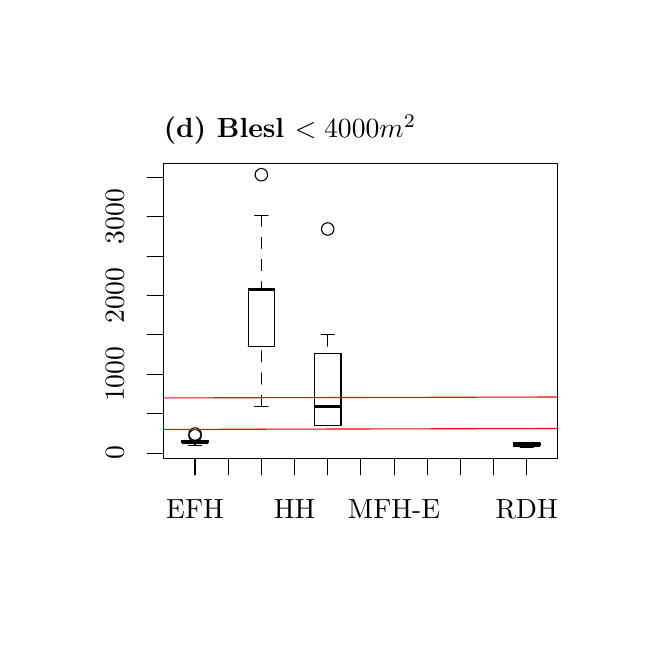
\begin{tikzpicture}[x=1pt,y=1pt]
\definecolor[named]{fillColor}{rgb}{1.00,1.00,1.00}
\path[use as bounding box,fill=fillColor,fill opacity=0.00] (0,0) rectangle (216.81,216.81);
\begin{scope}
\path[clip] ( 49.20, 61.20) rectangle (191.61,167.61);
\definecolor[named]{drawColor}{rgb}{0.00,0.00,0.00}

\path[draw=drawColor,line width= 1.2pt,line join=round] ( 55.67, 67.13) -- ( 65.26, 67.13);

\path[draw=drawColor,line width= 0.4pt,dash pattern=on 4pt off 4pt ,line join=round,line cap=round] ( 60.47, 65.97) -- ( 60.47, 66.91);

\path[draw=drawColor,line width= 0.4pt,dash pattern=on 4pt off 4pt ,line join=round,line cap=round] ( 60.47, 67.67) -- ( 60.47, 67.67);

\path[draw=drawColor,line width= 0.4pt,line join=round,line cap=round] ( 58.07, 65.97) -- ( 62.87, 65.97);

\path[draw=drawColor,line width= 0.4pt,line join=round,line cap=round] ( 58.07, 67.67) -- ( 62.87, 67.67);

\path[draw=drawColor,line width= 0.4pt,line join=round,line cap=round] ( 55.67, 66.91) --
	( 65.26, 66.91) --
	( 65.26, 67.67) --
	( 55.67, 67.67) --
	( 55.67, 66.91);

\path[draw=drawColor,line width= 0.4pt,line join=round,line cap=round] ( 60.47, 69.35) circle (  2.25);

\path[draw=drawColor,line width= 0.4pt,line join=round,line cap=round] ( 60.47, 69.98) circle (  2.25);

\path[draw=drawColor,line width= 1.2pt,line join=round] ( 79.65,122.15) -- ( 89.24,122.15);

\path[draw=drawColor,line width= 0.4pt,dash pattern=on 4pt off 4pt ,line join=round,line cap=round] ( 84.44, 80.03) -- ( 84.44,101.48);

\path[draw=drawColor,line width= 0.4pt,dash pattern=on 4pt off 4pt ,line join=round,line cap=round] ( 84.44,149.04) -- ( 84.44,122.15);

\path[draw=drawColor,line width= 0.4pt,line join=round,line cap=round] ( 82.05, 80.03) -- ( 86.84, 80.03);

\path[draw=drawColor,line width= 0.4pt,line join=round,line cap=round] ( 82.05,149.04) -- ( 86.84,149.04);

\path[draw=drawColor,line width= 0.4pt,line join=round,line cap=round] ( 79.65,101.48) --
	( 89.24,101.48) --
	( 89.24,122.15) --
	( 79.65,122.15) --
	( 79.65,101.48);

\path[draw=drawColor,line width= 0.4pt,line join=round,line cap=round] ( 84.44,163.67) circle (  2.25);

\path[draw=drawColor,line width= 1.2pt,line join=round] (103.62, 80.03) -- (113.21, 80.03);

\path[draw=drawColor,line width= 0.4pt,dash pattern=on 4pt off 4pt ,line join=round,line cap=round] (108.42, 73.02) -- (108.42, 73.08);

\path[draw=drawColor,line width= 0.4pt,dash pattern=on 4pt off 4pt ,line join=round,line cap=round] (108.42,105.78) -- (108.42, 99.04);

\path[draw=drawColor,line width= 0.4pt,line join=round,line cap=round] (106.02, 73.02) -- (110.82, 73.02);

\path[draw=drawColor,line width= 0.4pt,line join=round,line cap=round] (106.02,105.78) -- (110.82,105.78);

\path[draw=drawColor,line width= 0.4pt,line join=round,line cap=round] (103.62, 73.08) --
	(113.21, 73.08) --
	(113.21, 99.04) --
	(103.62, 99.04) --
	(103.62, 73.08);

\path[draw=drawColor,line width= 0.4pt,line join=round,line cap=round] (108.42,144.06) circle (  2.25);

\path[draw=drawColor,line width= 1.2pt,line join=round] (175.55, 66.02) -- (185.14, 66.02);

\path[draw=drawColor,line width= 0.4pt,dash pattern=on 4pt off 4pt ,line join=round,line cap=round] (180.34, 65.14) -- (180.34, 65.85);

\path[draw=drawColor,line width= 0.4pt,dash pattern=on 4pt off 4pt ,line join=round,line cap=round] (180.34, 66.96) -- (180.34, 66.73);

\path[draw=drawColor,line width= 0.4pt,line join=round,line cap=round] (177.94, 65.14) -- (182.74, 65.14);

\path[draw=drawColor,line width= 0.4pt,line join=round,line cap=round] (177.94, 66.96) -- (182.74, 66.96);

\path[draw=drawColor,line width= 0.4pt,line join=round,line cap=round] (175.55, 65.85) --
	(185.14, 65.85) --
	(185.14, 66.73) --
	(175.55, 66.73) --
	(175.55, 65.85);
\end{scope}
\begin{scope}
\path[clip] (  0.00,  0.00) rectangle (216.81,216.81);
\definecolor[named]{drawColor}{rgb}{0.00,0.00,0.00}

\path[draw=drawColor,line width= 0.4pt,line join=round,line cap=round] ( 60.47, 61.20) -- (180.34, 61.20);

\path[draw=drawColor,line width= 0.4pt,line join=round,line cap=round] ( 60.47, 61.20) -- ( 60.47, 55.20);

\path[draw=drawColor,line width= 0.4pt,line join=round,line cap=round] ( 72.46, 61.20) -- ( 72.46, 55.20);

\path[draw=drawColor,line width= 0.4pt,line join=round,line cap=round] ( 84.44, 61.20) -- ( 84.44, 55.20);

\path[draw=drawColor,line width= 0.4pt,line join=round,line cap=round] ( 96.43, 61.20) -- ( 96.43, 55.20);

\path[draw=drawColor,line width= 0.4pt,line join=round,line cap=round] (108.42, 61.20) -- (108.42, 55.20);

\path[draw=drawColor,line width= 0.4pt,line join=round,line cap=round] (120.41, 61.20) -- (120.41, 55.20);

\path[draw=drawColor,line width= 0.4pt,line join=round,line cap=round] (132.39, 61.20) -- (132.39, 55.20);

\path[draw=drawColor,line width= 0.4pt,line join=round,line cap=round] (144.38, 61.20) -- (144.38, 55.20);

\path[draw=drawColor,line width= 0.4pt,line join=round,line cap=round] (156.37, 61.20) -- (156.37, 55.20);

\path[draw=drawColor,line width= 0.4pt,line join=round,line cap=round] (168.35, 61.20) -- (168.35, 55.20);

\path[draw=drawColor,line width= 0.4pt,line join=round,line cap=round] (180.34, 61.20) -- (180.34, 55.20);

\node[text=drawColor,anchor=base,inner sep=0pt, outer sep=0pt, scale=  1.00] at ( 60.47, 39.60) {EFH};

\node[text=drawColor,anchor=base,inner sep=0pt, outer sep=0pt, scale=  1.00] at ( 96.43, 39.60) {HH};

\node[text=drawColor,anchor=base,inner sep=0pt, outer sep=0pt, scale=  1.00] at (132.39, 39.60) {MFH-E};

\node[text=drawColor,anchor=base,inner sep=0pt, outer sep=0pt, scale=  1.00] at (180.34, 39.60) {RDH};

\path[draw=drawColor,line width= 0.4pt,line join=round,line cap=round] ( 49.20, 63.09) -- ( 49.20,162.70);

\path[draw=drawColor,line width= 0.4pt,line join=round,line cap=round] ( 49.20, 63.09) -- ( 43.20, 63.09);

\path[draw=drawColor,line width= 0.4pt,line join=round,line cap=round] ( 49.20, 77.32) -- ( 43.20, 77.32);

\path[draw=drawColor,line width= 0.4pt,line join=round,line cap=round] ( 49.20, 91.55) -- ( 43.20, 91.55);

\path[draw=drawColor,line width= 0.4pt,line join=round,line cap=round] ( 49.20,105.78) -- ( 43.20,105.78);

\path[draw=drawColor,line width= 0.4pt,line join=round,line cap=round] ( 49.20,120.01) -- ( 43.20,120.01);

\path[draw=drawColor,line width= 0.4pt,line join=round,line cap=round] ( 49.20,134.24) -- ( 43.20,134.24);

\path[draw=drawColor,line width= 0.4pt,line join=round,line cap=round] ( 49.20,148.47) -- ( 43.20,148.47);

\path[draw=drawColor,line width= 0.4pt,line join=round,line cap=round] ( 49.20,162.70) -- ( 43.20,162.70);

\node[text=drawColor,rotate= 90.00,anchor=base,inner sep=0pt, outer sep=0pt, scale=  1.00] at ( 34.80, 63.09) {0};

\node[text=drawColor,rotate= 90.00,anchor=base,inner sep=0pt, outer sep=0pt, scale=  1.00] at ( 34.80, 91.55) {1000};

\node[text=drawColor,rotate= 90.00,anchor=base,inner sep=0pt, outer sep=0pt, scale=  1.00] at ( 34.80,120.01) {2000};

\node[text=drawColor,rotate= 90.00,anchor=base,inner sep=0pt, outer sep=0pt, scale=  1.00] at ( 34.80,148.47) {3000};

\node[text=drawColor,anchor=west, inner sep=0pt, outer sep=0pt, scale=  1.00]
at (49.20,180) {\textbf{(d) Blesl $< 4000 m^2$}
\label{fig:AreaBleslB}
};

\path[draw=drawColor,line width= 0.4pt,line join=round,line cap=round] ( 49.20, 61.20) --
	(191.61, 61.20) --
	(191.61,167.61) --
	( 49.20,167.61) --
	( 49.20, 61.20);
\end{scope}
\begin{scope}
\path[clip] ( 49.20, 61.20) rectangle (191.61,167.61);
\definecolor[named]{drawColor}{rgb}{1.00,0.00,0.00}

\path[draw=drawColor,line width= 0.4pt,line join=round,line cap=round] ( 49.20, 71.63) -- (191.61, 71.97);

\path[draw=drawColor,line width= 0.4pt,line join=round,line cap=round] ( 49.20, 83.02) -- (191.61, 83.35);
\end{scope}
\end{tikzpicture}
& \vspace{-3cm} 
%\hspace{-3.8cm}
% Created by tikzDevice version 0.6.2-92-0ad2792 on 2013-10-13 23:59:58
% !TEX encoding = UTF-8 Unicode
\begin{tikzpicture}[x=1pt,y=1pt]
\definecolor[named]{fillColor}{rgb}{1.00,1.00,1.00}
\path[use as bounding box,fill=fillColor,fill opacity=0.00] (0,0) rectangle (216.81,216.81);
\begin{scope}
\path[clip] ( 49.20, 61.20) rectangle (191.61,167.61);
\definecolor[named]{drawColor}{rgb}{0.00,0.00,0.00}

\path[draw=drawColor,line width= 1.2pt,line join=round] ( 55.67, 66.85) -- ( 65.26, 66.85);

\path[draw=drawColor,line width= 0.4pt,dash pattern=on 4pt off 4pt ,line join=round,line cap=round] ( 60.47, 65.54) -- ( 60.47, 66.33);

\path[draw=drawColor,line width= 0.4pt,dash pattern=on 4pt off 4pt ,line join=round,line cap=round] ( 60.47, 70.51) -- ( 60.47, 68.34);

\path[draw=drawColor,line width= 0.4pt,line join=round,line cap=round] ( 58.07, 65.54) -- ( 62.87, 65.54);

\path[draw=drawColor,line width= 0.4pt,line join=round,line cap=round] ( 58.07, 70.51) -- ( 62.87, 70.51);

\path[draw=drawColor,line width= 0.4pt,line join=round,line cap=round] ( 55.67, 66.33) --
	( 65.26, 66.33) --
	( 65.26, 68.34) --
	( 55.67, 68.34) --
	( 55.67, 66.33);

\path[draw=drawColor,line width= 1.2pt,line join=round] ( 79.65,104.30) -- ( 89.24,104.30);

\path[draw=drawColor,line width= 0.4pt,dash pattern=on 4pt off 4pt ,line join=round,line cap=round] ( 84.44, 84.20) -- ( 84.44,101.21);

\path[draw=drawColor,line width= 0.4pt,dash pattern=on 4pt off 4pt ,line join=round,line cap=round] ( 84.44,163.67) -- ( 84.44,148.98);

\path[draw=drawColor,line width= 0.4pt,line join=round,line cap=round] ( 82.05, 84.20) -- ( 86.84, 84.20);

\path[draw=drawColor,line width= 0.4pt,line join=round,line cap=round] ( 82.05,163.67) -- ( 86.84,163.67);

\path[draw=drawColor,line width= 0.4pt,line join=round,line cap=round] ( 79.65,101.21) --
	( 89.24,101.21) --
	( 89.24,148.98) --
	( 79.65,148.98) --
	( 79.65,101.21);

\path[draw=drawColor,line width= 1.2pt,line join=round] (103.62, 79.95) -- (113.21, 79.95);

\path[draw=drawColor,line width= 0.4pt,dash pattern=on 4pt off 4pt ,line join=round,line cap=round] (108.42, 70.77) -- (108.42, 74.83);

\path[draw=drawColor,line width= 0.4pt,dash pattern=on 4pt off 4pt ,line join=round,line cap=round] (108.42, 84.34) -- (108.42, 84.34);

\path[draw=drawColor,line width= 0.4pt,line join=round,line cap=round] (106.02, 70.77) -- (110.82, 70.77);

\path[draw=drawColor,line width= 0.4pt,line join=round,line cap=round] (106.02, 84.34) -- (110.82, 84.34);

\path[draw=drawColor,line width= 0.4pt,line join=round,line cap=round] (103.62, 74.83) --
	(113.21, 74.83) --
	(113.21, 84.34) --
	(103.62, 84.34) --
	(103.62, 74.83);

\path[draw=drawColor,line width= 0.4pt,line join=round,line cap=round] (108.42,143.96) circle (  2.25);

\path[draw=drawColor,line width= 0.4pt,line join=round,line cap=round] (108.42,119.56) circle (  2.25);

\path[draw=drawColor,line width= 1.2pt,line join=round] (175.55, 65.70) -- (185.14, 65.70);

\path[draw=drawColor,line width= 0.4pt,dash pattern=on 4pt off 4pt ,line join=round,line cap=round] (180.34, 65.14) -- (180.34, 65.46);

\path[draw=drawColor,line width= 0.4pt,dash pattern=on 4pt off 4pt ,line join=round,line cap=round] (180.34, 66.60) -- (180.34, 66.52);

\path[draw=drawColor,line width= 0.4pt,line join=round,line cap=round] (177.94, 65.14) -- (182.74, 65.14);

\path[draw=drawColor,line width= 0.4pt,line join=round,line cap=round] (177.94, 66.60) -- (182.74, 66.60);

\path[draw=drawColor,line width= 0.4pt,line join=round,line cap=round] (175.55, 65.46) --
	(185.14, 65.46) --
	(185.14, 66.52) --
	(175.55, 66.52) --
	(175.55, 65.46);
\end{scope}
\begin{scope}
\path[clip] (  0.00,  0.00) rectangle (216.81,216.81);
\definecolor[named]{drawColor}{rgb}{0.00,0.00,0.00}

\path[draw=drawColor,line width= 0.4pt,line join=round,line cap=round] ( 60.47, 61.20) -- (180.34, 61.20);

\path[draw=drawColor,line width= 0.4pt,line join=round,line cap=round] ( 60.47, 61.20) -- ( 60.47, 55.20);

\path[draw=drawColor,line width= 0.4pt,line join=round,line cap=round] ( 72.46, 61.20) -- ( 72.46, 55.20);

\path[draw=drawColor,line width= 0.4pt,line join=round,line cap=round] ( 84.44, 61.20) -- ( 84.44, 55.20);

\path[draw=drawColor,line width= 0.4pt,line join=round,line cap=round] ( 96.43, 61.20) -- ( 96.43, 55.20);

\path[draw=drawColor,line width= 0.4pt,line join=round,line cap=round] (108.42, 61.20) -- (108.42, 55.20);

\path[draw=drawColor,line width= 0.4pt,line join=round,line cap=round] (120.41, 61.20) -- (120.41, 55.20);

\path[draw=drawColor,line width= 0.4pt,line join=round,line cap=round] (132.39, 61.20) -- (132.39, 55.20);

\path[draw=drawColor,line width= 0.4pt,line join=round,line cap=round] (144.38, 61.20) -- (144.38, 55.20);

\path[draw=drawColor,line width= 0.4pt,line join=round,line cap=round] (156.37, 61.20) -- (156.37, 55.20);

\path[draw=drawColor,line width= 0.4pt,line join=round,line cap=round] (168.35, 61.20) -- (168.35, 55.20);

\path[draw=drawColor,line width= 0.4pt,line join=round,line cap=round] (180.34, 61.20) -- (180.34, 55.20);

% \node[text=drawColor,anchor=base,inner sep=0pt, outer sep=0pt, scale=  1.00] at ( 60.47, 39.60) {EFH};
% 
% \node[text=drawColor,anchor=base,inner sep=0pt, outer sep=0pt, scale=  1.00] at ( 96.43, 39.60) {HH};
% 
% \node[text=drawColor,anchor=base,inner sep=0pt, outer sep=0pt, scale=  1.00] at (132.39, 39.60) {MFH-E};
% 
% \node[text=drawColor,anchor=base,inner sep=0pt, outer sep=0pt, scale=  1.00] at (180.34, 39.60) {RDH};

\path[draw=drawColor,line width= 0.4pt,line join=round,line cap=round] ( 49.20, 62.65) -- ( 49.20,162.70);

\path[draw=drawColor,line width= 0.4pt,line join=round,line cap=round] ( 49.20, 62.65) -- ( 43.20, 62.65);

\path[draw=drawColor,line width= 0.4pt,line join=round,line cap=round] ( 49.20, 76.94) -- ( 43.20, 76.94);

\path[draw=drawColor,line width= 0.4pt,line join=round,line cap=round] ( 49.20, 91.23) -- ( 43.20, 91.23);

\path[draw=drawColor,line width= 0.4pt,line join=round,line cap=round] ( 49.20,105.53) -- ( 43.20,105.53);

\path[draw=drawColor,line width= 0.4pt,line join=round,line cap=round] ( 49.20,119.82) -- ( 43.20,119.82);

\path[draw=drawColor,line width= 0.4pt,line join=round,line cap=round] ( 49.20,134.11) -- ( 43.20,134.11);

\path[draw=drawColor,line width= 0.4pt,line join=round,line cap=round] ( 49.20,148.40) -- ( 43.20,148.40);

\path[draw=drawColor,line width= 0.4pt,line join=round,line cap=round] ( 49.20,162.70) -- ( 43.20,162.70);

% \node[text=drawColor,rotate= 90.00,anchor=base,inner sep=0pt, outer sep=0pt, scale=  1.00] at ( 34.80, 62.65) {0};
% 
% \node[text=drawColor,rotate= 90.00,anchor=base,inner sep=0pt, outer sep=0pt, scale=  1.00] at ( 34.80, 91.23) {1000};
% 
% \node[text=drawColor,rotate= 90.00,anchor=base,inner sep=0pt, outer sep=0pt, scale=  1.00] at ( 34.80,119.82) {2000};
% 
% \node[text=drawColor,rotate= 90.00,anchor=base,inner sep=0pt, outer sep=0pt, scale=  1.00] at ( 34.80,148.40) {3000};

\node[text=drawColor,anchor=west, inner sep=0pt, outer sep=0pt, scale=  1.00]
at (49.20,180) {\textbf{(e) IWU-de $< 4000 m^2$}
\label{fig:AreaIWUheA}
};

\path[draw=drawColor,line width= 0.4pt,line join=round,line cap=round] ( 49.20, 61.20) --
	(191.61, 61.20) --
	(191.61,167.61) --
	( 49.20,167.61) --
	( 49.20, 61.20);
\end{scope}
\begin{scope}
\path[clip] ( 49.20, 61.20) rectangle (191.61,167.61);
\definecolor[named]{drawColor}{rgb}{1.00,0.00,0.00}

\path[draw=drawColor,line width= 0.4pt,line join=round,line cap=round] ( 49.20, 71.23) -- (191.61, 71.57);

\path[draw=drawColor,line width= 0.4pt,line join=round,line cap=round] ( 49.20, 82.66) -- (191.61, 83.00);
\end{scope}
\end{tikzpicture}& \vspace{-3cm}
%\hspace{-3.8cm}
% Created by tikzDevice version 0.6.2-92-0ad2792 on 2013-10-13 23:59:59
% !TEX encoding = UTF-8 Unicode
\begin{tikzpicture}[x=1pt,y=1pt]
\definecolor[named]{fillColor}{rgb}{1.00,1.00,1.00}
\path[use as bounding box,fill=fillColor,fill opacity=0.00] (0,0) rectangle (216.81,216.81);
\begin{scope}
\path[clip] ( 49.20, 61.20) rectangle (191.61,167.61);
\definecolor[named]{drawColor}{rgb}{0.00,0.00,0.00}

\path[draw=drawColor,line width= 1.2pt,line join=round] ( 55.67, 67.46) -- ( 65.26, 67.46);

\path[draw=drawColor,line width= 0.4pt,dash pattern=on 4pt off 4pt ,line join=round,line cap=round] ( 60.47, 65.54) -- ( 60.47, 66.46);

\path[draw=drawColor,line width= 0.4pt,dash pattern=on 4pt off 4pt ,line join=round,line cap=round] ( 60.47, 70.51) -- ( 60.47, 68.91);

\path[draw=drawColor,line width= 0.4pt,line join=round,line cap=round] ( 58.07, 65.54) -- ( 62.87, 65.54);

\path[draw=drawColor,line width= 0.4pt,line join=round,line cap=round] ( 58.07, 70.51) -- ( 62.87, 70.51);

\path[draw=drawColor,line width= 0.4pt,line join=round,line cap=round] ( 55.67, 66.46) --
	( 65.26, 66.46) --
	( 65.26, 68.91) --
	( 55.67, 68.91) --
	( 55.67, 66.46);

\path[draw=drawColor,line width= 1.2pt,line join=round] ( 67.66, 67.76) -- ( 77.25, 67.76);

\path[draw=drawColor,line width= 0.4pt,dash pattern=on 4pt off 4pt ,line join=round,line cap=round] ( 72.46, 67.17) -- ( 72.46, 67.17);

\path[draw=drawColor,line width= 0.4pt,dash pattern=on 4pt off 4pt ,line join=round,line cap=round] ( 72.46, 68.34) -- ( 72.46, 68.34);

\path[draw=drawColor,line width= 0.4pt,line join=round,line cap=round] ( 70.06, 67.17) -- ( 74.85, 67.17);

\path[draw=drawColor,line width= 0.4pt,line join=round,line cap=round] ( 70.06, 68.34) -- ( 74.85, 68.34);

\path[draw=drawColor,line width= 0.4pt,line join=round,line cap=round] ( 67.66, 67.17) --
	( 77.25, 67.17) --
	( 77.25, 68.34) --
	( 67.66, 68.34) --
	( 67.66, 67.17);

\path[draw=drawColor,line width= 1.2pt,line join=round] ( 79.65,104.30) -- ( 89.24,104.30);

\path[draw=drawColor,line width= 0.4pt,dash pattern=on 4pt off 4pt ,line join=round,line cap=round] ( 84.44, 84.21) -- ( 84.44,101.21);

\path[draw=drawColor,line width= 0.4pt,dash pattern=on 4pt off 4pt ,line join=round,line cap=round] ( 84.44,163.67) -- ( 84.44,148.98);

\path[draw=drawColor,line width= 0.4pt,line join=round,line cap=round] ( 82.05, 84.21) -- ( 86.84, 84.21);

\path[draw=drawColor,line width= 0.4pt,line join=round,line cap=round] ( 82.05,163.67) -- ( 86.84,163.67);

\path[draw=drawColor,line width= 0.4pt,line join=round,line cap=round] ( 79.65,101.21) --
	( 89.24,101.21) --
	( 89.24,148.98) --
	( 79.65,148.98) --
	( 79.65,101.21);

\path[draw=drawColor,line width= 1.2pt,line join=round] (103.62, 79.66) -- (113.21, 79.66);

\path[draw=drawColor,line width= 0.4pt,dash pattern=on 4pt off 4pt ,line join=round,line cap=round] (108.42, 72.66) -- (108.42, 76.96);

\path[draw=drawColor,line width= 0.4pt,dash pattern=on 4pt off 4pt ,line join=round,line cap=round] (108.42, 82.86) -- (108.42, 81.56);

\path[draw=drawColor,line width= 0.4pt,line join=round,line cap=round] (106.02, 72.66) -- (110.82, 72.66);

\path[draw=drawColor,line width= 0.4pt,line join=round,line cap=round] (106.02, 82.86) -- (110.82, 82.86);

\path[draw=drawColor,line width= 0.4pt,line join=round,line cap=round] (103.62, 76.96) --
	(113.21, 76.96) --
	(113.21, 81.56) --
	(103.62, 81.56) --
	(103.62, 76.96);

\path[draw=drawColor,line width= 0.4pt,line join=round,line cap=round] (108.42,143.97) circle (  2.25);

\path[draw=drawColor,line width= 1.2pt,line join=round] (115.61, 70.77) -- (125.20, 70.77);

\path[draw=drawColor,line width= 0.4pt,dash pattern=on 4pt off 4pt ,line join=round,line cap=round] (120.41, 70.77) -- (120.41, 70.77);

\path[draw=drawColor,line width= 0.4pt,dash pattern=on 4pt off 4pt ,line join=round,line cap=round] (120.41, 70.77) -- (120.41, 70.77);

\path[draw=drawColor,line width= 0.4pt,line join=round,line cap=round] (118.01, 70.77) -- (122.80, 70.77);

\path[draw=drawColor,line width= 0.4pt,line join=round,line cap=round] (118.01, 70.77) -- (122.80, 70.77);

\path[draw=drawColor,line width= 0.4pt,line join=round,line cap=round] (115.61, 70.77) --
	(125.20, 70.77) --
	(125.20, 70.77) --
	(115.61, 70.77) --
	(115.61, 70.77);

\path[draw=drawColor,line width= 1.2pt,line join=round] (175.55, 65.60) -- (185.14, 65.60);

\path[draw=drawColor,line width= 0.4pt,dash pattern=on 4pt off 4pt ,line join=round,line cap=round] (180.34, 65.14) -- (180.34, 65.44);

\path[draw=drawColor,line width= 0.4pt,dash pattern=on 4pt off 4pt ,line join=round,line cap=round] (180.34, 65.97) -- (180.34, 65.84);

\path[draw=drawColor,line width= 0.4pt,line join=round,line cap=round] (177.94, 65.14) -- (182.74, 65.14);

\path[draw=drawColor,line width= 0.4pt,line join=round,line cap=round] (177.94, 65.97) -- (182.74, 65.97);

\path[draw=drawColor,line width= 0.4pt,line join=round,line cap=round] (175.55, 65.44) --
	(185.14, 65.44) --
	(185.14, 65.84) --
	(175.55, 65.84) --
	(175.55, 65.44);

\path[draw=drawColor,line width= 0.4pt,line join=round,line cap=round] (180.34, 66.54) circle (  2.25);
\end{scope}
\begin{scope}
\path[clip] (  0.00,  0.00) rectangle (216.81,216.81);
\definecolor[named]{drawColor}{rgb}{0.00,0.00,0.00}

\path[draw=drawColor,line width= 0.4pt,line join=round,line cap=round] ( 60.47, 61.20) -- (180.34, 61.20);

\path[draw=drawColor,line width= 0.4pt,line join=round,line cap=round] ( 60.47, 61.20) -- ( 60.47, 55.20);

\path[draw=drawColor,line width= 0.4pt,line join=round,line cap=round] ( 72.46, 61.20) -- ( 72.46, 55.20);

\path[draw=drawColor,line width= 0.4pt,line join=round,line cap=round] ( 84.44, 61.20) -- ( 84.44, 55.20);

\path[draw=drawColor,line width= 0.4pt,line join=round,line cap=round] ( 96.43, 61.20) -- ( 96.43, 55.20);

\path[draw=drawColor,line width= 0.4pt,line join=round,line cap=round] (108.42, 61.20) -- (108.42, 55.20);

\path[draw=drawColor,line width= 0.4pt,line join=round,line cap=round] (120.41, 61.20) -- (120.41, 55.20);

\path[draw=drawColor,line width= 0.4pt,line join=round,line cap=round] (132.39, 61.20) -- (132.39, 55.20);

\path[draw=drawColor,line width= 0.4pt,line join=round,line cap=round] (144.38, 61.20) -- (144.38, 55.20);

\path[draw=drawColor,line width= 0.4pt,line join=round,line cap=round] (156.37, 61.20) -- (156.37, 55.20);

\path[draw=drawColor,line width= 0.4pt,line join=round,line cap=round] (168.35, 61.20) -- (168.35, 55.20);

\path[draw=drawColor,line width= 0.4pt,line join=round,line cap=round] (180.34, 61.20) -- (180.34, 55.20);

% \node[text=drawColor,anchor=base,inner sep=0pt, outer sep=0pt, scale=  1.00] at ( 60.47, 39.60) {EFH};
% 
% \node[text=drawColor,anchor=base,inner sep=0pt, outer sep=0pt, scale=  1.00] at ( 96.43, 39.60) {HH};
% 
% \node[text=drawColor,anchor=base,inner sep=0pt, outer sep=0pt, scale=  1.00] at (132.39, 39.60) {MFH-E};
% 
% \node[text=drawColor,anchor=base,inner sep=0pt, outer sep=0pt, scale=  1.00] at (180.34, 39.60) {RDH};

\path[draw=drawColor,line width= 0.4pt,line join=round,line cap=round] ( 49.20, 62.65) -- ( 49.20,162.70);

\path[draw=drawColor,line width= 0.4pt,line join=round,line cap=round] ( 49.20, 62.65) -- ( 43.20, 62.65);

\path[draw=drawColor,line width= 0.4pt,line join=round,line cap=round] ( 49.20, 76.95) -- ( 43.20, 76.95);

\path[draw=drawColor,line width= 0.4pt,line join=round,line cap=round] ( 49.20, 91.24) -- ( 43.20, 91.24);

\path[draw=drawColor,line width= 0.4pt,line join=round,line cap=round] ( 49.20,105.53) -- ( 43.20,105.53);

\path[draw=drawColor,line width= 0.4pt,line join=round,line cap=round] ( 49.20,119.82) -- ( 43.20,119.82);

\path[draw=drawColor,line width= 0.4pt,line join=round,line cap=round] ( 49.20,134.11) -- ( 43.20,134.11);

\path[draw=drawColor,line width= 0.4pt,line join=round,line cap=round] ( 49.20,148.41) -- ( 43.20,148.41);

\path[draw=drawColor,line width= 0.4pt,line join=round,line cap=round] ( 49.20,162.70) -- ( 43.20,162.70);

% \node[text=drawColor,rotate= 90.00,anchor=base,inner sep=0pt, outer sep=0pt, scale=  1.00] at ( 34.80, 62.65) {0};
% 
% \node[text=drawColor,rotate= 90.00,anchor=base,inner sep=0pt, outer sep=0pt, scale=  1.00] at ( 34.80, 91.24) {1000};
% 
% \node[text=drawColor,rotate= 90.00,anchor=base,inner sep=0pt, outer sep=0pt, scale=  1.00] at ( 34.80,119.82) {2000};
% 
% \node[text=drawColor,rotate= 90.00,anchor=base,inner sep=0pt, outer sep=0pt, scale=  1.00] at ( 34.80,148.41) {3000};

\node[text=drawColor,anchor=west, inner sep=0pt, outer sep=0pt, scale=  1.00]
at (49.20,180) {\textbf{(f) IWU-he $< 4000 m^2$}
\label{fig:AreaIWUheA}
};

\path[draw=drawColor,line width= 0.4pt,line join=round,line cap=round] ( 49.20, 61.20) --
	(191.61, 61.20) --
	(191.61,167.61) --
	( 49.20,167.61) --
	( 49.20, 61.20);
\end{scope}
\begin{scope}
\path[clip] ( 49.20, 61.20) rectangle (191.61,167.61);
\definecolor[named]{drawColor}{rgb}{1.00,0.00,0.00}

\path[draw=drawColor,line width= 0.4pt,line join=round,line cap=round] ( 49.20, 71.23) -- (191.61, 71.57);

\path[draw=drawColor,line width= 0.4pt,line join=round,line cap=round] ( 49.20, 82.66) -- (191.61, 83.00);
\end{scope}
\end{tikzpicture}
\\
    \end{tabular}
    
\vspace{-1.6cm}
\begin{flushright}
\footnotesize{data source:
(a-d)~\cite{Blesl.2007}
(b-e)~\cite{Loga.2011}
(c-f)~\cite{Born.2003}
}
\end{flushright}
	\caption[Different values for living space of building typologies used in
	Germany.]{Different values for living space of building typologies used in
	Germany.
    The building types are arrange by construction type in alphabetical order
    along the X-axis.
	The Y-axis shows the living space of the single typologies in
	$[m^2]$.
	EFH; EFH-b; GMH; HH; KMH; KMH-b; MFH-E; MFH-G; MFH-H; MFH-W; RDH}
    \label{fig:DifTypArea}
\end{figure}


\subsubsection{Number of Floors}

The number of floors are directly retrieved from the digital cadaster.  This
parameter is define in some of the typologies and can help us to classify the
buildings between construction types.  This parameter is only used with the
float array filter (see Sub-Section~\ref{sub-sec:filter} for a detail
description of the array filter), as defining this parameter in the binary
filter my lead to be inconsistencies within the data.  E.g.: a building in the
digital cadaster may have no possible type because it eliminates all possible
types, if the building is of construction type (KMH) and is 10 stories high.
In the defined typology, a particular building may be correctly attributed a
construction type, but may be filtered out, because of a deterministic
definition of a limit in the number of stories category.  In the float array
this will only decrease the probability of a type being peeked out.\\

The ``rules'' for the attribution of probabilities for the individual types, as
function of number of stories, works similar to the attribution of
probabilities as function of the living space (see sub
Sub-Section~\ref{sub-sec:livings}). In Table~\ref{tab:pst} the number of
stories for the different types of two typologies (iwu-he and ecofyz) are
plotted along with the defined limits needed for the probability definition.
The definition of this probabilities can be seen in Table~\ref{tab:pst}.\\

\begin{table}[htb]
  \centering
  \caption{Probabilities assign to building types as function of number of
  stories}
  \label{tab:pst}
  \begin{tabular}{rcr rrrr}

    \toprule
    &&&
    EFH (a)  & KMH (d)   & GMH (g)   & HH (j) \\ 
    &&&
    EFH-b (b)& KMH-b (e)& MFH-G (h)& MFH-H (k)\\
    \multicolumn{3}{c}{\textbf{\# stories}}& 
    %\multicolumn{3}{c}{$[m^2]$}& 
    RDH (c)   & MFH-E (f)& MFH-W (i)& \\
    \midrule
\textless &-&    4     & 1.0 & 0.6 & 0.0 & 0.0 \\
        4 &-&    5     & 0.6 & 1.0 & 0.6 & 0.0 \\
        6 &-&    9     & 0.0 & 0.6 & 1.0 & 0.6 \\
        9 &-&   15     & 0.0 & 0.0 & 0.6 & 1.0 \\
\textgreater  &-&   15     & 0.0 & 0.0 & 0.0 & 1.0 \\
    \bottomrule
  \end{tabular}
\end{table}

\begin{figure}[htb]
\centering
%\textbf{Number of stories for construction types of two typologies}\\

\hspace{-2.5cm}
  \begin{tabular}{p{0.5\linewidth} p{0.5\linewidth} }

\textbf{(a) IWU-he (table~\ref{tab:IWU-he})}&
\textbf{(b) EcoFYZ (table~\ref{tab:EcoFYZ})}
\\
%\hspace{-1.4cm}
%\\ 
\vspace{-2cm}
% Created by tikzDevice version 0.8.1 on 2015-03-03 13:54:09
% !TEX encoding = UTF-8 Unicode
\begin{tikzpicture}[x=1pt,y=1pt]
\definecolor{fillColor}{RGB}{255,255,255}
\path[use as bounding box,fill=fillColor,fill opacity=0.00] (0,0) rectangle (216.81,216.81);
\begin{scope}
\path[clip] ( 49.20, 61.20) rectangle (191.61,167.61);
\definecolor{drawColor}{RGB}{0,0,0}

\path[draw=drawColor,line width= 1.2pt,line join=round] ( 55.67, 74.99) -- ( 65.26, 74.99);

\path[draw=drawColor,line width= 0.4pt,dash pattern=on 4pt off 4pt ,line join=round,line cap=round] ( 60.47, 74.99) -- ( 60.47, 74.99);

\path[draw=drawColor,line width= 0.4pt,dash pattern=on 4pt off 4pt ,line join=round,line cap=round] ( 60.47, 74.99) -- ( 60.47, 74.99);

\path[draw=drawColor,line width= 0.4pt,line join=round,line cap=round] ( 58.07, 74.99) -- ( 62.87, 74.99);

\path[draw=drawColor,line width= 0.4pt,line join=round,line cap=round] ( 58.07, 74.99) -- ( 62.87, 74.99);

\path[draw=drawColor,line width= 0.4pt,line join=round,line cap=round] ( 55.67, 74.99) --
	( 65.26, 74.99) --
	( 65.26, 74.99) --
	( 55.67, 74.99) --
	( 55.67, 74.99);

\path[draw=drawColor,line width= 1.2pt,line join=round] ( 67.66, 74.99) -- ( 77.25, 74.99);

\path[draw=drawColor,line width= 0.4pt,dash pattern=on 4pt off 4pt ,line join=round,line cap=round] ( 72.46, 74.99) -- ( 72.46, 74.99);

\path[draw=drawColor,line width= 0.4pt,dash pattern=on 4pt off 4pt ,line join=round,line cap=round] ( 72.46, 74.99) -- ( 72.46, 74.99);

\path[draw=drawColor,line width= 0.4pt,line join=round,line cap=round] ( 70.06, 74.99) -- ( 74.85, 74.99);

\path[draw=drawColor,line width= 0.4pt,line join=round,line cap=round] ( 70.06, 74.99) -- ( 74.85, 74.99);

\path[draw=drawColor,line width= 0.4pt,line join=round,line cap=round] ( 67.66, 74.99) --
	( 77.25, 74.99) --
	( 77.25, 74.99) --
	( 67.66, 74.99) --
	( 67.66, 74.99);

\path[draw=drawColor,line width= 1.2pt,line join=round] ( 79.65, 89.77) -- ( 89.24, 89.77);

\path[draw=drawColor,line width= 0.4pt,dash pattern=on 4pt off 4pt ,line join=round,line cap=round] ( 84.44, 89.77) -- ( 84.44, 89.77);

\path[draw=drawColor,line width= 0.4pt,dash pattern=on 4pt off 4pt ,line join=round,line cap=round] ( 84.44,109.48) -- ( 84.44,109.48);

\path[draw=drawColor,line width= 0.4pt,line join=round,line cap=round] ( 82.05, 89.77) -- ( 86.84, 89.77);

\path[draw=drawColor,line width= 0.4pt,line join=round,line cap=round] ( 82.05,109.48) -- ( 86.84,109.48);

\path[draw=drawColor,line width= 0.4pt,line join=round,line cap=round] ( 79.65, 89.77) --
	( 89.24, 89.77) --
	( 89.24,109.48) --
	( 79.65,109.48) --
	( 79.65, 89.77);

\path[draw=drawColor,line width= 1.2pt,line join=round] ( 91.64,151.35) -- (101.23,151.35);

\path[draw=drawColor,line width= 0.4pt,dash pattern=on 4pt off 4pt ,line join=round,line cap=round] ( 96.43,139.04) -- ( 96.43,139.04);

\path[draw=drawColor,line width= 0.4pt,dash pattern=on 4pt off 4pt ,line join=round,line cap=round] ( 96.43,163.67) -- ( 96.43,163.67);

\path[draw=drawColor,line width= 0.4pt,line join=round,line cap=round] ( 94.03,139.04) -- ( 98.83,139.04);

\path[draw=drawColor,line width= 0.4pt,line join=round,line cap=round] ( 94.03,163.67) -- ( 98.83,163.67);

\path[draw=drawColor,line width= 0.4pt,line join=round,line cap=round] ( 91.64,139.04) --
	(101.23,139.04) --
	(101.23,163.67) --
	( 91.64,163.67) --
	( 91.64,139.04);

\path[draw=drawColor,line width= 1.2pt,line join=round] (103.62, 79.92) -- (113.21, 79.92);

\path[draw=drawColor,line width= 0.4pt,dash pattern=on 4pt off 4pt ,line join=round,line cap=round] (108.42, 79.92) -- (108.42, 79.92);

\path[draw=drawColor,line width= 0.4pt,dash pattern=on 4pt off 4pt ,line join=round,line cap=round] (108.42, 89.77) -- (108.42, 89.77);

\path[draw=drawColor,line width= 0.4pt,line join=round,line cap=round] (106.02, 79.92) -- (110.82, 79.92);

\path[draw=drawColor,line width= 0.4pt,line join=round,line cap=round] (106.02, 89.77) -- (110.82, 89.77);

\path[draw=drawColor,line width= 0.4pt,line join=round,line cap=round] (103.62, 79.92) --
	(113.21, 79.92) --
	(113.21, 89.77) --
	(103.62, 89.77) --
	(103.62, 79.92);

\path[draw=drawColor,line width= 1.2pt,line join=round] (115.61, 89.77) -- (125.20, 89.77);

\path[draw=drawColor,line width= 0.4pt,dash pattern=on 4pt off 4pt ,line join=round,line cap=round] (120.41, 89.77) -- (120.41, 89.77);

\path[draw=drawColor,line width= 0.4pt,dash pattern=on 4pt off 4pt ,line join=round,line cap=round] (120.41, 89.77) -- (120.41, 89.77);

\path[draw=drawColor,line width= 0.4pt,line join=round,line cap=round] (118.01, 89.77) -- (122.80, 89.77);

\path[draw=drawColor,line width= 0.4pt,line join=round,line cap=round] (118.01, 89.77) -- (122.80, 89.77);

\path[draw=drawColor,line width= 0.4pt,line join=round,line cap=round] (115.61, 89.77) --
	(125.20, 89.77) --
	(125.20, 89.77) --
	(115.61, 89.77) --
	(115.61, 89.77);

\path[draw=drawColor,line width= 1.2pt,line join=round] (175.55, 74.99) -- (185.14, 74.99);

\path[draw=drawColor,line width= 0.4pt,dash pattern=on 4pt off 4pt ,line join=round,line cap=round] (180.34, 74.99) -- (180.34, 74.99);

\path[draw=drawColor,line width= 0.4pt,dash pattern=on 4pt off 4pt ,line join=round,line cap=round] (180.34, 74.99) -- (180.34, 74.99);

\path[draw=drawColor,line width= 0.4pt,line join=round,line cap=round] (177.94, 74.99) -- (182.74, 74.99);

\path[draw=drawColor,line width= 0.4pt,line join=round,line cap=round] (177.94, 74.99) -- (182.74, 74.99);

\path[draw=drawColor,line width= 0.4pt,line join=round,line cap=round] (175.55, 74.99) --
	(185.14, 74.99) --
	(185.14, 74.99) --
	(175.55, 74.99) --
	(175.55, 74.99);
\end{scope}
\begin{scope}
\path[clip] (  0.00,  0.00) rectangle (216.81,216.81);
\definecolor{drawColor}{RGB}{0,0,0}

\path[draw=drawColor,line width= 0.4pt,line join=round,line cap=round] ( 60.47, 61.20) -- (180.34, 61.20);

\path[draw=drawColor,line width= 0.4pt,line join=round,line cap=round] ( 60.47, 61.20) -- ( 60.47, 55.20);

\path[draw=drawColor,line width= 0.4pt,line join=round,line cap=round] ( 72.46, 61.20) -- ( 72.46, 55.20);

\path[draw=drawColor,line width= 0.4pt,line join=round,line cap=round] ( 84.44, 61.20) -- ( 84.44, 55.20);

\path[draw=drawColor,line width= 0.4pt,line join=round,line cap=round] ( 96.43, 61.20) -- ( 96.43, 55.20);

\path[draw=drawColor,line width= 0.4pt,line join=round,line cap=round] (108.42, 61.20) -- (108.42, 55.20);

\path[draw=drawColor,line width= 0.4pt,line join=round,line cap=round] (120.41, 61.20) -- (120.41, 55.20);

\path[draw=drawColor,line width= 0.4pt,line join=round,line cap=round] (132.39, 61.20) -- (132.39, 55.20);

\path[draw=drawColor,line width= 0.4pt,line join=round,line cap=round] (144.38, 61.20) -- (144.38, 55.20);

\path[draw=drawColor,line width= 0.4pt,line join=round,line cap=round] (156.37, 61.20) -- (156.37, 55.20);

\path[draw=drawColor,line width= 0.4pt,line join=round,line cap=round] (168.35, 61.20) -- (168.35, 55.20);

\path[draw=drawColor,line width= 0.4pt,line join=round,line cap=round] (180.34, 61.20) -- (180.34, 55.20);

\node[text=drawColor,anchor=base,inner sep=0pt, outer sep=0pt, scale=  1.00] at ( 60.47, 39.60) {EFH};

\node[text=drawColor,anchor=base,inner sep=0pt, outer sep=0pt, scale=  1.00] at ( 96.43, 39.60) {HH};

\node[text=drawColor,anchor=base,inner sep=0pt, outer sep=0pt, scale=  1.00] at (132.39, 39.60) {MFH-E};

\node[text=drawColor,anchor=base,inner sep=0pt, outer sep=0pt, scale=  1.00] at (180.34, 39.60) {RDH};

\path[draw=drawColor,line width= 0.4pt,line join=round,line cap=round] ( 49.20, 65.14) -- ( 49.20,163.67);

\path[draw=drawColor,line width= 0.4pt,line join=round,line cap=round] ( 49.20, 65.14) -- ( 43.20, 65.14);

\path[draw=drawColor,line width= 0.4pt,line join=round,line cap=round] ( 49.20, 89.77) -- ( 43.20, 89.77);

\path[draw=drawColor,line width= 0.4pt,line join=round,line cap=round] ( 49.20,114.40) -- ( 43.20,114.40);

\path[draw=drawColor,line width= 0.4pt,line join=round,line cap=round] ( 49.20,139.04) -- ( 43.20,139.04);

\path[draw=drawColor,line width= 0.4pt,line join=round,line cap=round] ( 49.20,163.67) -- ( 43.20,163.67);

\node[text=drawColor,rotate= 90.00,anchor=base,inner sep=0pt, outer sep=0pt, scale=  1.00] at ( 34.80, 65.14) {0};

\node[text=drawColor,rotate= 90.00,anchor=base,inner sep=0pt, outer sep=0pt, scale=  1.00] at ( 34.80, 89.77) {5};

\node[text=drawColor,rotate= 90.00,anchor=base,inner sep=0pt, outer sep=0pt, scale=  1.00] at ( 34.80,114.40) {10};

\node[text=drawColor,rotate= 90.00,anchor=base,inner sep=0pt, outer sep=0pt, scale=  1.00] at ( 34.80,139.04) {15};

\node[text=drawColor,rotate= 90.00,anchor=base,inner sep=0pt, outer sep=0pt, scale=  1.00] at ( 34.80,163.67) {20};

\path[draw=drawColor,line width= 0.4pt,line join=round,line cap=round] ( 49.20, 61.20) --
	(191.61, 61.20) --
	(191.61,167.61) --
	( 49.20,167.61) --
	( 49.20, 61.20);
\end{scope}
\begin{scope}
\path[clip] ( 49.20, 61.20) rectangle (191.61,167.61);
\definecolor{drawColor}{RGB}{255,0,0}

\path[draw=drawColor,line width= 0.4pt,line join=round,line cap=round] ( 49.20, 89.77) -- (191.61, 89.77);

\path[draw=drawColor,line width= 0.4pt,line join=round,line cap=round] ( 49.20,139.04) -- (191.61,139.04);
\end{scope}
<<<<<<< HEAD
\end{tikzpicture}
=======
\end{tikzpicture}
>>>>>>> 36a956db0f2ffb15b4b8091da9293464a1b25a0c
&
\vspace{-2cm}
% Created by tikzDevice version 0.8.1 on 2015-03-03 13:54:10
% !TEX encoding = UTF-8 Unicode
\begin{tikzpicture}[x=1pt,y=1pt]
\definecolor{fillColor}{RGB}{255,255,255}
\path[use as bounding box,fill=fillColor,fill opacity=0.00] (0,0) rectangle (216.81,216.81);
\begin{scope}
\path[clip] ( 49.20, 61.20) rectangle (191.61,167.61);
\definecolor{drawColor}{RGB}{0,0,0}

\path[draw=drawColor,line width= 1.2pt,line join=round] ( 55.67, 74.99) -- ( 65.26, 74.99);

\path[draw=drawColor,line width= 0.4pt,dash pattern=on 4pt off 4pt ,line join=round,line cap=round] ( 60.47, 74.99) -- ( 60.47, 74.99);

\path[draw=drawColor,line width= 0.4pt,dash pattern=on 4pt off 4pt ,line join=round,line cap=round] ( 60.47, 74.99) -- ( 60.47, 74.99);

\path[draw=drawColor,line width= 0.4pt,line join=round,line cap=round] ( 58.07, 74.99) -- ( 62.87, 74.99);

\path[draw=drawColor,line width= 0.4pt,line join=round,line cap=round] ( 58.07, 74.99) -- ( 62.87, 74.99);

\path[draw=drawColor,line width= 0.4pt,line join=round,line cap=round] ( 55.67, 74.99) --
	( 65.26, 74.99) --
	( 65.26, 74.99) --
	( 55.67, 74.99) --
	( 55.67, 74.99);

\path[draw=drawColor,line width= 1.2pt,line join=round] (127.60, 74.99) -- (137.19, 74.99);

\path[draw=drawColor,line width= 0.4pt,dash pattern=on 4pt off 4pt ,line join=round,line cap=round] (132.39, 74.99) -- (132.39, 74.99);

\path[draw=drawColor,line width= 0.4pt,dash pattern=on 4pt off 4pt ,line join=round,line cap=round] (132.39, 74.99) -- (132.39, 74.99);

\path[draw=drawColor,line width= 0.4pt,line join=round,line cap=round] (129.99, 74.99) -- (134.79, 74.99);

\path[draw=drawColor,line width= 0.4pt,line join=round,line cap=round] (129.99, 74.99) -- (134.79, 74.99);

\path[draw=drawColor,line width= 0.4pt,line join=round,line cap=round] (127.60, 74.99) --
	(137.19, 74.99) --
	(137.19, 74.99) --
	(127.60, 74.99) --
	(127.60, 74.99);

\path[draw=drawColor,line width= 0.4pt,line join=round,line cap=round] (132.39, 79.92) circle (  2.25);

\path[draw=drawColor,line width= 1.2pt,line join=round] (139.58, 89.77) -- (149.17, 89.77);

\path[draw=drawColor,line width= 0.4pt,dash pattern=on 4pt off 4pt ,line join=round,line cap=round] (144.38, 89.77) -- (144.38, 89.77);

\path[draw=drawColor,line width= 0.4pt,dash pattern=on 4pt off 4pt ,line join=round,line cap=round] (144.38, 89.77) -- (144.38, 89.77);

\path[draw=drawColor,line width= 0.4pt,line join=round,line cap=round] (141.98, 89.77) -- (146.78, 89.77);

\path[draw=drawColor,line width= 0.4pt,line join=round,line cap=round] (141.98, 89.77) -- (146.78, 89.77);

\path[draw=drawColor,line width= 0.4pt,line join=round,line cap=round] (139.58, 89.77) --
	(149.17, 89.77) --
	(149.17, 89.77) --
	(139.58, 89.77) --
	(139.58, 89.77);

\path[draw=drawColor,line width= 1.2pt,line join=round] (151.57,119.33) -- (161.16,119.33);

\path[draw=drawColor,line width= 0.4pt,dash pattern=on 4pt off 4pt ,line join=round,line cap=round] (156.37,109.48) -- (156.37,109.48);

\path[draw=drawColor,line width= 0.4pt,dash pattern=on 4pt off 4pt ,line join=round,line cap=round] (156.37,129.18) -- (156.37,129.18);

\path[draw=drawColor,line width= 0.4pt,line join=round,line cap=round] (153.97,109.48) -- (158.76,109.48);

\path[draw=drawColor,line width= 0.4pt,line join=round,line cap=round] (153.97,129.18) -- (158.76,129.18);

\path[draw=drawColor,line width= 0.4pt,line join=round,line cap=round] (151.57,109.48) --
	(161.16,109.48) --
	(161.16,129.18) --
	(151.57,129.18) --
	(151.57,109.48);

\path[draw=drawColor,line width= 1.2pt,line join=round] (163.56, 89.77) -- (173.15, 89.77);

\path[draw=drawColor,line width= 0.4pt,dash pattern=on 4pt off 4pt ,line join=round,line cap=round] (168.35, 89.77) -- (168.35, 89.77);

\path[draw=drawColor,line width= 0.4pt,dash pattern=on 4pt off 4pt ,line join=round,line cap=round] (168.35, 89.77) -- (168.35, 89.77);

\path[draw=drawColor,line width= 0.4pt,line join=round,line cap=round] (165.96, 89.77) -- (170.75, 89.77);

\path[draw=drawColor,line width= 0.4pt,line join=round,line cap=round] (165.96, 89.77) -- (170.75, 89.77);

\path[draw=drawColor,line width= 0.4pt,line join=round,line cap=round] (163.56, 89.77) --
	(173.15, 89.77) --
	(173.15, 89.77) --
	(163.56, 89.77) --
	(163.56, 89.77);

\path[draw=drawColor,line width= 1.2pt,line join=round] (175.55, 74.99) -- (185.14, 74.99);

\path[draw=drawColor,line width= 0.4pt,dash pattern=on 4pt off 4pt ,line join=round,line cap=round] (180.34, 74.99) -- (180.34, 74.99);

\path[draw=drawColor,line width= 0.4pt,dash pattern=on 4pt off 4pt ,line join=round,line cap=round] (180.34, 74.99) -- (180.34, 74.99);

\path[draw=drawColor,line width= 0.4pt,line join=round,line cap=round] (177.94, 74.99) -- (182.74, 74.99);

\path[draw=drawColor,line width= 0.4pt,line join=round,line cap=round] (177.94, 74.99) -- (182.74, 74.99);

\path[draw=drawColor,line width= 0.4pt,line join=round,line cap=round] (175.55, 74.99) --
	(185.14, 74.99) --
	(185.14, 74.99) --
	(175.55, 74.99) --
	(175.55, 74.99);
\end{scope}
\begin{scope}
\path[clip] (  0.00,  0.00) rectangle (216.81,216.81);
\definecolor{drawColor}{RGB}{0,0,0}

\path[draw=drawColor,line width= 0.4pt,line join=round,line cap=round] ( 60.47, 61.20) -- (180.34, 61.20);

\path[draw=drawColor,line width= 0.4pt,line join=round,line cap=round] ( 60.47, 61.20) -- ( 60.47, 55.20);

\path[draw=drawColor,line width= 0.4pt,line join=round,line cap=round] ( 72.46, 61.20) -- ( 72.46, 55.20);

\path[draw=drawColor,line width= 0.4pt,line join=round,line cap=round] ( 84.44, 61.20) -- ( 84.44, 55.20);

\path[draw=drawColor,line width= 0.4pt,line join=round,line cap=round] ( 96.43, 61.20) -- ( 96.43, 55.20);

\path[draw=drawColor,line width= 0.4pt,line join=round,line cap=round] (108.42, 61.20) -- (108.42, 55.20);

\path[draw=drawColor,line width= 0.4pt,line join=round,line cap=round] (120.41, 61.20) -- (120.41, 55.20);

\path[draw=drawColor,line width= 0.4pt,line join=round,line cap=round] (132.39, 61.20) -- (132.39, 55.20);

\path[draw=drawColor,line width= 0.4pt,line join=round,line cap=round] (144.38, 61.20) -- (144.38, 55.20);

\path[draw=drawColor,line width= 0.4pt,line join=round,line cap=round] (156.37, 61.20) -- (156.37, 55.20);

\path[draw=drawColor,line width= 0.4pt,line join=round,line cap=round] (168.35, 61.20) -- (168.35, 55.20);

\path[draw=drawColor,line width= 0.4pt,line join=round,line cap=round] (180.34, 61.20) -- (180.34, 55.20);

\node[text=drawColor,anchor=base,inner sep=0pt, outer sep=0pt, scale=  1.00] at ( 60.47, 39.60) {EFH};

\node[text=drawColor,anchor=base,inner sep=0pt, outer sep=0pt, scale=  1.00] at ( 96.43, 39.60) {HH};

\node[text=drawColor,anchor=base,inner sep=0pt, outer sep=0pt, scale=  1.00] at (132.39, 39.60) {MFH-E};

\node[text=drawColor,anchor=base,inner sep=0pt, outer sep=0pt, scale=  1.00] at (180.34, 39.60) {RDH};

\path[draw=drawColor,line width= 0.4pt,line join=round,line cap=round] ( 49.20, 65.14) -- ( 49.20,163.67);

\path[draw=drawColor,line width= 0.4pt,line join=round,line cap=round] ( 49.20, 65.14) -- ( 43.20, 65.14);

\path[draw=drawColor,line width= 0.4pt,line join=round,line cap=round] ( 49.20, 89.77) -- ( 43.20, 89.77);

\path[draw=drawColor,line width= 0.4pt,line join=round,line cap=round] ( 49.20,114.40) -- ( 43.20,114.40);

\path[draw=drawColor,line width= 0.4pt,line join=round,line cap=round] ( 49.20,139.04) -- ( 43.20,139.04);

\path[draw=drawColor,line width= 0.4pt,line join=round,line cap=round] ( 49.20,163.67) -- ( 43.20,163.67);

\node[text=drawColor,rotate= 90.00,anchor=base,inner sep=0pt, outer sep=0pt, scale=  1.00] at ( 34.80, 65.14) {0};

\node[text=drawColor,rotate= 90.00,anchor=base,inner sep=0pt, outer sep=0pt, scale=  1.00] at ( 34.80, 89.77) {5};

\node[text=drawColor,rotate= 90.00,anchor=base,inner sep=0pt, outer sep=0pt, scale=  1.00] at ( 34.80,114.40) {10};

\node[text=drawColor,rotate= 90.00,anchor=base,inner sep=0pt, outer sep=0pt, scale=  1.00] at ( 34.80,139.04) {15};

\node[text=drawColor,rotate= 90.00,anchor=base,inner sep=0pt, outer sep=0pt, scale=  1.00] at ( 34.80,163.67) {20};

\path[draw=drawColor,line width= 0.4pt,line join=round,line cap=round] ( 49.20, 61.20) --
	(191.61, 61.20) --
	(191.61,167.61) --
	( 49.20,167.61) --
	( 49.20, 61.20);
\end{scope}
\begin{scope}
\path[clip] ( 49.20, 61.20) rectangle (191.61,167.61);
\definecolor{drawColor}{RGB}{255,0,0}

\path[draw=drawColor,line width= 0.4pt,line join=round,line cap=round] ( 49.20, 89.77) -- (191.61, 89.77);

\path[draw=drawColor,line width= 0.4pt,line join=round,line cap=round] ( 49.20,139.04) -- (191.61,139.04);
\end{scope}
\end{tikzpicture}\\
  \end{tabular}
\vspace{-1.4cm}

\begin{flushright}
\footnotesize{data source:~\cite{Born.2003,Hermelink.2011}}
\end{flushright}
	\caption[Different values for number of floors of building typologies used in
	Germany.]{Different values for number of floors of building typologies used in
	Germany.
	The building types are arrange by construction type in alphabetical order along
	the X-axis.
	The Y-axis shows the number of stories of the individual typologies.
	EFH; EFH-b; GMH; HH; KMH; KMH-b; MFH-E; MFH-G; MFH-H; MFH-W; RDH}
	\label{fig:DifTypFloor}
\end{figure}

\subsubsection{Roof Type}

Some of the typologies define the type of roof of the individual types.
Because we can gather this information from the digital cadaster, the parameter
can be used to classify the buildings.  This parameter is only used with the
float array filter (see Sub-Section~\ref{sub-sec:filter} for a detail
description of the filter array). Figure~\ref{fig:DifTypRoof} shows the
different roof types per construction type for two typologies.\\

\begin{figure}[htb]
\centering
\textbf{Roof types for construction types of two typologies}\\
%\vspace{-0.6cm} 

  \begin{tabular}{p{0.5\textwidth} p{0.5\textwidth}}

\hspace{-1.4cm}
% Created by tikzDevice version 0.8.1 on 2015-03-03 13:54:10
% !TEX encoding = UTF-8 Unicode
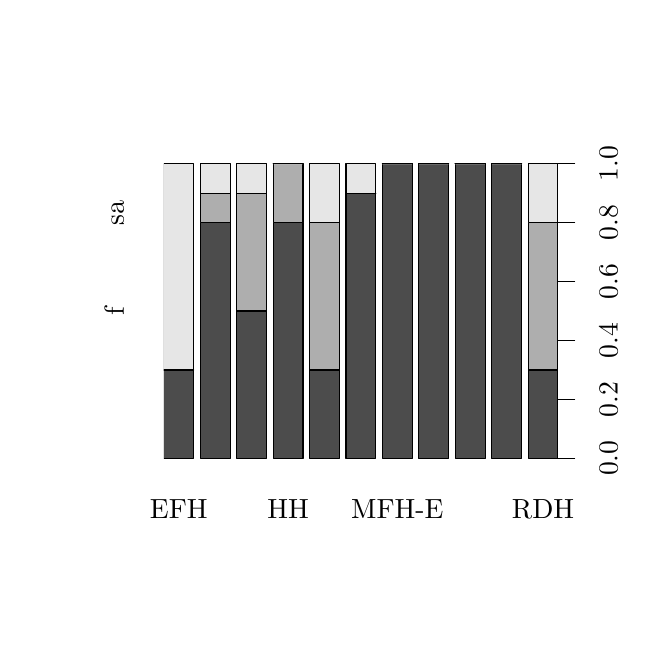
\begin{tikzpicture}[x=1pt,y=1pt]
\definecolor{fillColor}{RGB}{255,255,255}
\path[use as bounding box,fill=fillColor,fill opacity=0.00] (0,0) rectangle (216.81,216.81);
\begin{scope}
\path[clip] (  0.00,  0.00) rectangle (216.81,216.81);
\definecolor{drawColor}{RGB}{0,0,0}

\end{scope}
\begin{scope}
\path[clip] ( 49.20, 61.20) rectangle (191.61,167.61);
\definecolor{drawColor}{RGB}{0,0,0}
\definecolor{fillColor}{gray}{0.30}

\path[draw=drawColor,line width= 0.4pt,line join=round,line cap=round,fill=fillColor] ( 49.20, 61.20) rectangle ( 59.99, 93.12);
\definecolor{fillColor}{RGB}{174,174,174}

\path[draw=drawColor,line width= 0.4pt,line join=round,line cap=round,fill=fillColor] ( 49.20, 93.12) rectangle ( 59.99, 93.12);
\definecolor{fillColor}{RGB}{230,230,230}

\path[draw=drawColor,line width= 0.4pt,line join=round,line cap=round,fill=fillColor] ( 49.20, 93.12) rectangle ( 59.99,167.61);
\definecolor{fillColor}{gray}{0.30}

\path[draw=drawColor,line width= 0.4pt,line join=round,line cap=round,fill=fillColor] ( 62.36, 61.20) rectangle ( 73.15,146.33);
\definecolor{fillColor}{RGB}{174,174,174}

\path[draw=drawColor,line width= 0.4pt,line join=round,line cap=round,fill=fillColor] ( 62.36,146.33) rectangle ( 73.15,156.97);
\definecolor{fillColor}{RGB}{230,230,230}

\path[draw=drawColor,line width= 0.4pt,line join=round,line cap=round,fill=fillColor] ( 62.36,156.97) rectangle ( 73.15,167.61);
\definecolor{fillColor}{gray}{0.30}

\path[draw=drawColor,line width= 0.4pt,line join=round,line cap=round,fill=fillColor] ( 75.52, 61.20) rectangle ( 86.31,114.41);
\definecolor{fillColor}{RGB}{174,174,174}

\path[draw=drawColor,line width= 0.4pt,line join=round,line cap=round,fill=fillColor] ( 75.52,114.41) rectangle ( 86.31,156.97);
\definecolor{fillColor}{RGB}{230,230,230}

\path[draw=drawColor,line width= 0.4pt,line join=round,line cap=round,fill=fillColor] ( 75.52,156.97) rectangle ( 86.31,167.61);
\definecolor{fillColor}{gray}{0.30}

\path[draw=drawColor,line width= 0.4pt,line join=round,line cap=round,fill=fillColor] ( 88.69, 61.20) rectangle ( 99.48,146.33);
\definecolor{fillColor}{RGB}{174,174,174}

\path[draw=drawColor,line width= 0.4pt,line join=round,line cap=round,fill=fillColor] ( 88.69,146.33) rectangle ( 99.48,167.61);
\definecolor{fillColor}{RGB}{230,230,230}

\path[draw=drawColor,line width= 0.4pt,line join=round,line cap=round,fill=fillColor] ( 88.69,167.61) rectangle ( 99.48,167.61);
\definecolor{fillColor}{gray}{0.30}

\path[draw=drawColor,line width= 0.4pt,line join=round,line cap=round,fill=fillColor] (101.85, 61.20) rectangle (112.64, 93.12);
\definecolor{fillColor}{RGB}{174,174,174}

\path[draw=drawColor,line width= 0.4pt,line join=round,line cap=round,fill=fillColor] (101.85, 93.12) rectangle (112.64,146.33);
\definecolor{fillColor}{RGB}{230,230,230}

\path[draw=drawColor,line width= 0.4pt,line join=round,line cap=round,fill=fillColor] (101.85,146.33) rectangle (112.64,167.61);
\definecolor{fillColor}{gray}{0.30}

\path[draw=drawColor,line width= 0.4pt,line join=round,line cap=round,fill=fillColor] (115.01, 61.20) rectangle (125.80,156.97);
\definecolor{fillColor}{RGB}{174,174,174}

\path[draw=drawColor,line width= 0.4pt,line join=round,line cap=round,fill=fillColor] (115.01,156.97) rectangle (125.80,156.97);
\definecolor{fillColor}{RGB}{230,230,230}

\path[draw=drawColor,line width= 0.4pt,line join=round,line cap=round,fill=fillColor] (115.01,156.97) rectangle (125.80,167.61);
\definecolor{fillColor}{gray}{0.30}

\path[draw=drawColor,line width= 0.4pt,line join=round,line cap=round,fill=fillColor] (128.17, 61.20) rectangle (138.96,167.61);
\definecolor{fillColor}{RGB}{174,174,174}

\path[draw=drawColor,line width= 0.4pt,line join=round,line cap=round,fill=fillColor] (128.17,167.61) rectangle (138.96,167.61);
\definecolor{fillColor}{RGB}{230,230,230}

\path[draw=drawColor,line width= 0.4pt,line join=round,line cap=round,fill=fillColor] (128.17,167.61) rectangle (138.96,167.61);
\definecolor{fillColor}{gray}{0.30}

\path[draw=drawColor,line width= 0.4pt,line join=round,line cap=round,fill=fillColor] (141.33, 61.20) rectangle (152.12,167.61);
\definecolor{fillColor}{RGB}{174,174,174}

\path[draw=drawColor,line width= 0.4pt,line join=round,line cap=round,fill=fillColor] (141.33,167.61) rectangle (152.12,167.61);
\definecolor{fillColor}{RGB}{230,230,230}

\path[draw=drawColor,line width= 0.4pt,line join=round,line cap=round,fill=fillColor] (141.33,167.61) rectangle (152.12,167.61);
\definecolor{fillColor}{gray}{0.30}

\path[draw=drawColor,line width= 0.4pt,line join=round,line cap=round,fill=fillColor] (154.50, 61.20) rectangle (165.29,167.61);
\definecolor{fillColor}{RGB}{174,174,174}

\path[draw=drawColor,line width= 0.4pt,line join=round,line cap=round,fill=fillColor] (154.50,167.61) rectangle (165.29,167.61);
\definecolor{fillColor}{RGB}{230,230,230}

\path[draw=drawColor,line width= 0.4pt,line join=round,line cap=round,fill=fillColor] (154.50,167.61) rectangle (165.29,167.61);
\definecolor{fillColor}{gray}{0.30}

\path[draw=drawColor,line width= 0.4pt,line join=round,line cap=round,fill=fillColor] (167.66, 61.20) rectangle (178.45,167.61);
\definecolor{fillColor}{RGB}{174,174,174}

\path[draw=drawColor,line width= 0.4pt,line join=round,line cap=round,fill=fillColor] (167.66,167.61) rectangle (178.45,167.61);
\definecolor{fillColor}{RGB}{230,230,230}

\path[draw=drawColor,line width= 0.4pt,line join=round,line cap=round,fill=fillColor] (167.66,167.61) rectangle (178.45,167.61);
\definecolor{fillColor}{gray}{0.30}

\path[draw=drawColor,line width= 0.4pt,line join=round,line cap=round,fill=fillColor] (180.82, 61.20) rectangle (191.61, 93.12);
\definecolor{fillColor}{RGB}{174,174,174}

\path[draw=drawColor,line width= 0.4pt,line join=round,line cap=round,fill=fillColor] (180.82, 93.12) rectangle (191.61,146.33);
\definecolor{fillColor}{RGB}{230,230,230}

\path[draw=drawColor,line width= 0.4pt,line join=round,line cap=round,fill=fillColor] (180.82,146.33) rectangle (191.61,167.61);
\end{scope}
\begin{scope}
\path[clip] (  0.00,  0.00) rectangle (216.81,216.81);
\definecolor{drawColor}{RGB}{0,0,0}

\node[text=drawColor,anchor=base,inner sep=0pt, outer sep=0pt, scale=  1.00] at ( 54.59, 39.60) {EFH};

\node[text=drawColor,anchor=base,inner sep=0pt, outer sep=0pt, scale=  1.00] at ( 94.08, 39.60) {HH};

\node[text=drawColor,anchor=base,inner sep=0pt, outer sep=0pt, scale=  1.00] at (133.57, 39.60) {MFH-E};

\node[text=drawColor,anchor=base,inner sep=0pt, outer sep=0pt, scale=  1.00] at (186.22, 39.60) {RDH};

\node[text=drawColor,rotate= 90.00,anchor=base,inner sep=0pt, outer sep=0pt, scale=  1.00] at ( 34.80,114.41) {f};

\node[text=drawColor,rotate= 90.00,anchor=base,inner sep=0pt, outer sep=0pt, scale=  1.00] at ( 34.80,149.88) {sa};

\path[draw=drawColor,line width= 0.4pt,line join=round,line cap=round] (191.61, 61.20) -- (191.61,167.61);

\path[draw=drawColor,line width= 0.4pt,line join=round,line cap=round] (191.61, 61.20) -- (197.61, 61.20);

\path[draw=drawColor,line width= 0.4pt,line join=round,line cap=round] (191.61, 82.48) -- (197.61, 82.48);

\path[draw=drawColor,line width= 0.4pt,line join=round,line cap=round] (191.61,103.76) -- (197.61,103.76);

\path[draw=drawColor,line width= 0.4pt,line join=round,line cap=round] (191.61,125.05) -- (197.61,125.05);

\path[draw=drawColor,line width= 0.4pt,line join=round,line cap=round] (191.61,146.33) -- (197.61,146.33);

\path[draw=drawColor,line width= 0.4pt,line join=round,line cap=round] (191.61,167.61) -- (197.61,167.61);

\node[text=drawColor,rotate= 90.00,anchor=base,inner sep=0pt, outer sep=0pt, scale=  1.00] at (213.21, 61.20) {0.0};

\node[text=drawColor,rotate= 90.00,anchor=base,inner sep=0pt, outer sep=0pt, scale=  1.00] at (213.21, 82.48) {0.2};

\node[text=drawColor,rotate= 90.00,anchor=base,inner sep=0pt, outer sep=0pt, scale=  1.00] at (213.21,103.76) {0.4};

\node[text=drawColor,rotate= 90.00,anchor=base,inner sep=0pt, outer sep=0pt, scale=  1.00] at (213.21,125.05) {0.6};

\node[text=drawColor,rotate= 90.00,anchor=base,inner sep=0pt, outer sep=0pt, scale=  1.00] at (213.21,146.33) {0.8};

\node[text=drawColor,rotate= 90.00,anchor=base,inner sep=0pt, outer sep=0pt, scale=  1.00] at (213.21,167.61) {1.0};
\end{scope}
<<<<<<< HEAD
\end{tikzpicture}
=======
\end{tikzpicture}
>>>>>>> 36a956db0f2ffb15b4b8091da9293464a1b25a0c
&
\hspace{-1.4cm}
% Created by tikzDevice version 0.8.1 on 2015-03-03 13:54:12
% !TEX encoding = UTF-8 Unicode
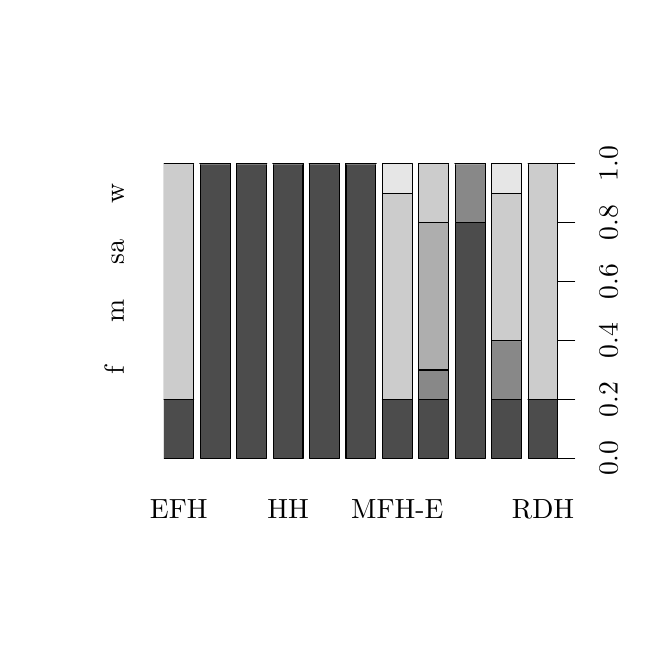
\begin{tikzpicture}[x=1pt,y=1pt]
\definecolor{fillColor}{RGB}{255,255,255}
\path[use as bounding box,fill=fillColor,fill opacity=0.00] (0,0) rectangle (216.81,216.81);
\begin{scope}
\path[clip] (  0.00,  0.00) rectangle (216.81,216.81);
\definecolor{drawColor}{RGB}{0,0,0}

\end{scope}
\begin{scope}
\path[clip] ( 49.20, 61.20) rectangle (191.61,167.61);
\definecolor{drawColor}{RGB}{0,0,0}
\definecolor{fillColor}{gray}{0.30}

\path[draw=drawColor,line width= 0.4pt,line join=round,line cap=round,fill=fillColor] ( 49.20, 61.20) rectangle ( 59.99, 82.48);
\definecolor{fillColor}{RGB}{136,136,136}

\path[draw=drawColor,line width= 0.4pt,line join=round,line cap=round,fill=fillColor] ( 49.20, 82.48) rectangle ( 59.99, 82.48);
\definecolor{fillColor}{RGB}{174,174,174}

\path[draw=drawColor,line width= 0.4pt,line join=round,line cap=round,fill=fillColor] ( 49.20, 82.48) rectangle ( 59.99, 82.48);
\definecolor{fillColor}{gray}{0.80}

\path[draw=drawColor,line width= 0.4pt,line join=round,line cap=round,fill=fillColor] ( 49.20, 82.48) rectangle ( 59.99,167.61);
\definecolor{fillColor}{RGB}{230,230,230}

\path[draw=drawColor,line width= 0.4pt,line join=round,line cap=round,fill=fillColor] ( 49.20,167.61) rectangle ( 59.99,167.61);
\definecolor{fillColor}{gray}{0.30}

\path[draw=drawColor,line width= 0.4pt,line join=round,line cap=round,fill=fillColor] ( 62.36, 61.20) rectangle ( 73.15,167.61);
\definecolor{fillColor}{RGB}{136,136,136}

\path[draw=drawColor,line width= 0.4pt,line join=round,line cap=round,fill=fillColor] ( 62.36,167.61) rectangle ( 73.15,167.61);
\definecolor{fillColor}{RGB}{174,174,174}

\path[draw=drawColor,line width= 0.4pt,line join=round,line cap=round,fill=fillColor] ( 62.36,167.61) rectangle ( 73.15,167.61);
\definecolor{fillColor}{gray}{0.80}

\path[draw=drawColor,line width= 0.4pt,line join=round,line cap=round,fill=fillColor] ( 62.36,167.61) rectangle ( 73.15,167.61);
\definecolor{fillColor}{RGB}{230,230,230}

\path[draw=drawColor,line width= 0.4pt,line join=round,line cap=round,fill=fillColor] ( 62.36,167.61) rectangle ( 73.15,167.61);
\definecolor{fillColor}{gray}{0.30}

\path[draw=drawColor,line width= 0.4pt,line join=round,line cap=round,fill=fillColor] ( 75.52, 61.20) rectangle ( 86.31,167.61);
\definecolor{fillColor}{RGB}{136,136,136}

\path[draw=drawColor,line width= 0.4pt,line join=round,line cap=round,fill=fillColor] ( 75.52,167.61) rectangle ( 86.31,167.61);
\definecolor{fillColor}{RGB}{174,174,174}

\path[draw=drawColor,line width= 0.4pt,line join=round,line cap=round,fill=fillColor] ( 75.52,167.61) rectangle ( 86.31,167.61);
\definecolor{fillColor}{gray}{0.80}

\path[draw=drawColor,line width= 0.4pt,line join=round,line cap=round,fill=fillColor] ( 75.52,167.61) rectangle ( 86.31,167.61);
\definecolor{fillColor}{RGB}{230,230,230}

\path[draw=drawColor,line width= 0.4pt,line join=round,line cap=round,fill=fillColor] ( 75.52,167.61) rectangle ( 86.31,167.61);
\definecolor{fillColor}{gray}{0.30}

\path[draw=drawColor,line width= 0.4pt,line join=round,line cap=round,fill=fillColor] ( 88.69, 61.20) rectangle ( 99.48,167.61);
\definecolor{fillColor}{RGB}{136,136,136}

\path[draw=drawColor,line width= 0.4pt,line join=round,line cap=round,fill=fillColor] ( 88.69,167.61) rectangle ( 99.48,167.61);
\definecolor{fillColor}{RGB}{174,174,174}

\path[draw=drawColor,line width= 0.4pt,line join=round,line cap=round,fill=fillColor] ( 88.69,167.61) rectangle ( 99.48,167.61);
\definecolor{fillColor}{gray}{0.80}

\path[draw=drawColor,line width= 0.4pt,line join=round,line cap=round,fill=fillColor] ( 88.69,167.61) rectangle ( 99.48,167.61);
\definecolor{fillColor}{RGB}{230,230,230}

\path[draw=drawColor,line width= 0.4pt,line join=round,line cap=round,fill=fillColor] ( 88.69,167.61) rectangle ( 99.48,167.61);
\definecolor{fillColor}{gray}{0.30}

\path[draw=drawColor,line width= 0.4pt,line join=round,line cap=round,fill=fillColor] (101.85, 61.20) rectangle (112.64,167.61);
\definecolor{fillColor}{RGB}{136,136,136}

\path[draw=drawColor,line width= 0.4pt,line join=round,line cap=round,fill=fillColor] (101.85,167.61) rectangle (112.64,167.61);
\definecolor{fillColor}{RGB}{174,174,174}

\path[draw=drawColor,line width= 0.4pt,line join=round,line cap=round,fill=fillColor] (101.85,167.61) rectangle (112.64,167.61);
\definecolor{fillColor}{gray}{0.80}

\path[draw=drawColor,line width= 0.4pt,line join=round,line cap=round,fill=fillColor] (101.85,167.61) rectangle (112.64,167.61);
\definecolor{fillColor}{RGB}{230,230,230}

\path[draw=drawColor,line width= 0.4pt,line join=round,line cap=round,fill=fillColor] (101.85,167.61) rectangle (112.64,167.61);
\definecolor{fillColor}{gray}{0.30}

\path[draw=drawColor,line width= 0.4pt,line join=round,line cap=round,fill=fillColor] (115.01, 61.20) rectangle (125.80,167.61);
\definecolor{fillColor}{RGB}{136,136,136}

\path[draw=drawColor,line width= 0.4pt,line join=round,line cap=round,fill=fillColor] (115.01,167.61) rectangle (125.80,167.61);
\definecolor{fillColor}{RGB}{174,174,174}

\path[draw=drawColor,line width= 0.4pt,line join=round,line cap=round,fill=fillColor] (115.01,167.61) rectangle (125.80,167.61);
\definecolor{fillColor}{gray}{0.80}

\path[draw=drawColor,line width= 0.4pt,line join=round,line cap=round,fill=fillColor] (115.01,167.61) rectangle (125.80,167.61);
\definecolor{fillColor}{RGB}{230,230,230}

\path[draw=drawColor,line width= 0.4pt,line join=round,line cap=round,fill=fillColor] (115.01,167.61) rectangle (125.80,167.61);
\definecolor{fillColor}{gray}{0.30}

\path[draw=drawColor,line width= 0.4pt,line join=round,line cap=round,fill=fillColor] (128.17, 61.20) rectangle (138.96, 82.48);
\definecolor{fillColor}{RGB}{136,136,136}

\path[draw=drawColor,line width= 0.4pt,line join=round,line cap=round,fill=fillColor] (128.17, 82.48) rectangle (138.96, 82.48);
\definecolor{fillColor}{RGB}{174,174,174}

\path[draw=drawColor,line width= 0.4pt,line join=round,line cap=round,fill=fillColor] (128.17, 82.48) rectangle (138.96, 82.48);
\definecolor{fillColor}{gray}{0.80}

\path[draw=drawColor,line width= 0.4pt,line join=round,line cap=round,fill=fillColor] (128.17, 82.48) rectangle (138.96,156.97);
\definecolor{fillColor}{RGB}{230,230,230}

\path[draw=drawColor,line width= 0.4pt,line join=round,line cap=round,fill=fillColor] (128.17,156.97) rectangle (138.96,167.61);
\definecolor{fillColor}{gray}{0.30}

\path[draw=drawColor,line width= 0.4pt,line join=round,line cap=round,fill=fillColor] (141.33, 61.20) rectangle (152.12, 82.48);
\definecolor{fillColor}{RGB}{136,136,136}

\path[draw=drawColor,line width= 0.4pt,line join=round,line cap=round,fill=fillColor] (141.33, 82.48) rectangle (152.12, 93.12);
\definecolor{fillColor}{RGB}{174,174,174}

\path[draw=drawColor,line width= 0.4pt,line join=round,line cap=round,fill=fillColor] (141.33, 93.12) rectangle (152.12,146.33);
\definecolor{fillColor}{gray}{0.80}

\path[draw=drawColor,line width= 0.4pt,line join=round,line cap=round,fill=fillColor] (141.33,146.33) rectangle (152.12,167.61);
\definecolor{fillColor}{RGB}{230,230,230}

\path[draw=drawColor,line width= 0.4pt,line join=round,line cap=round,fill=fillColor] (141.33,167.61) rectangle (152.12,167.61);
\definecolor{fillColor}{gray}{0.30}

\path[draw=drawColor,line width= 0.4pt,line join=round,line cap=round,fill=fillColor] (154.50, 61.20) rectangle (165.29,146.33);
\definecolor{fillColor}{RGB}{136,136,136}

\path[draw=drawColor,line width= 0.4pt,line join=round,line cap=round,fill=fillColor] (154.50,146.33) rectangle (165.29,167.61);
\definecolor{fillColor}{RGB}{174,174,174}

\path[draw=drawColor,line width= 0.4pt,line join=round,line cap=round,fill=fillColor] (154.50,167.61) rectangle (165.29,167.61);
\definecolor{fillColor}{gray}{0.80}

\path[draw=drawColor,line width= 0.4pt,line join=round,line cap=round,fill=fillColor] (154.50,167.61) rectangle (165.29,167.61);
\definecolor{fillColor}{RGB}{230,230,230}

\path[draw=drawColor,line width= 0.4pt,line join=round,line cap=round,fill=fillColor] (154.50,167.61) rectangle (165.29,167.61);
\definecolor{fillColor}{gray}{0.30}

\path[draw=drawColor,line width= 0.4pt,line join=round,line cap=round,fill=fillColor] (167.66, 61.20) rectangle (178.45, 82.48);
\definecolor{fillColor}{RGB}{136,136,136}

\path[draw=drawColor,line width= 0.4pt,line join=round,line cap=round,fill=fillColor] (167.66, 82.48) rectangle (178.45,103.76);
\definecolor{fillColor}{RGB}{174,174,174}

\path[draw=drawColor,line width= 0.4pt,line join=round,line cap=round,fill=fillColor] (167.66,103.76) rectangle (178.45,103.76);
\definecolor{fillColor}{gray}{0.80}

\path[draw=drawColor,line width= 0.4pt,line join=round,line cap=round,fill=fillColor] (167.66,103.76) rectangle (178.45,156.97);
\definecolor{fillColor}{RGB}{230,230,230}

\path[draw=drawColor,line width= 0.4pt,line join=round,line cap=round,fill=fillColor] (167.66,156.97) rectangle (178.45,167.61);
\definecolor{fillColor}{gray}{0.30}

\path[draw=drawColor,line width= 0.4pt,line join=round,line cap=round,fill=fillColor] (180.82, 61.20) rectangle (191.61, 82.48);
\definecolor{fillColor}{RGB}{136,136,136}

\path[draw=drawColor,line width= 0.4pt,line join=round,line cap=round,fill=fillColor] (180.82, 82.48) rectangle (191.61, 82.48);
\definecolor{fillColor}{RGB}{174,174,174}

\path[draw=drawColor,line width= 0.4pt,line join=round,line cap=round,fill=fillColor] (180.82, 82.48) rectangle (191.61, 82.48);
\definecolor{fillColor}{gray}{0.80}

\path[draw=drawColor,line width= 0.4pt,line join=round,line cap=round,fill=fillColor] (180.82, 82.48) rectangle (191.61,167.61);
\definecolor{fillColor}{RGB}{230,230,230}

\path[draw=drawColor,line width= 0.4pt,line join=round,line cap=round,fill=fillColor] (180.82,167.61) rectangle (191.61,167.61);
\end{scope}
\begin{scope}
\path[clip] (  0.00,  0.00) rectangle (216.81,216.81);
\definecolor{drawColor}{RGB}{0,0,0}

\node[text=drawColor,anchor=base,inner sep=0pt, outer sep=0pt, scale=  1.00] at ( 54.59, 39.60) {EFH};

\node[text=drawColor,anchor=base,inner sep=0pt, outer sep=0pt, scale=  1.00] at ( 94.08, 39.60) {HH};

\node[text=drawColor,anchor=base,inner sep=0pt, outer sep=0pt, scale=  1.00] at (133.57, 39.60) {MFH-E};

\node[text=drawColor,anchor=base,inner sep=0pt, outer sep=0pt, scale=  1.00] at (186.22, 39.60) {RDH};

\node[text=drawColor,rotate= 90.00,anchor=base,inner sep=0pt, outer sep=0pt, scale=  1.00] at ( 34.80, 93.12) {f};

\node[text=drawColor,rotate= 90.00,anchor=base,inner sep=0pt, outer sep=0pt, scale=  1.00] at ( 34.80,114.41) {m};

\node[text=drawColor,rotate= 90.00,anchor=base,inner sep=0pt, outer sep=0pt, scale=  1.00] at ( 34.80,135.69) {sa};

\node[text=drawColor,rotate= 90.00,anchor=base,inner sep=0pt, outer sep=0pt, scale=  1.00] at ( 34.80,156.97) {w};

\path[draw=drawColor,line width= 0.4pt,line join=round,line cap=round] (191.61, 61.20) -- (191.61,167.61);

\path[draw=drawColor,line width= 0.4pt,line join=round,line cap=round] (191.61, 61.20) -- (197.61, 61.20);

\path[draw=drawColor,line width= 0.4pt,line join=round,line cap=round] (191.61, 82.48) -- (197.61, 82.48);

\path[draw=drawColor,line width= 0.4pt,line join=round,line cap=round] (191.61,103.76) -- (197.61,103.76);

\path[draw=drawColor,line width= 0.4pt,line join=round,line cap=round] (191.61,125.05) -- (197.61,125.05);

\path[draw=drawColor,line width= 0.4pt,line join=round,line cap=round] (191.61,146.33) -- (197.61,146.33);

\path[draw=drawColor,line width= 0.4pt,line join=round,line cap=round] (191.61,167.61) -- (197.61,167.61);

\node[text=drawColor,rotate= 90.00,anchor=base,inner sep=0pt, outer sep=0pt, scale=  1.00] at (213.21, 61.20) {0.0};

\node[text=drawColor,rotate= 90.00,anchor=base,inner sep=0pt, outer sep=0pt, scale=  1.00] at (213.21, 82.48) {0.2};

\node[text=drawColor,rotate= 90.00,anchor=base,inner sep=0pt, outer sep=0pt, scale=  1.00] at (213.21,103.76) {0.4};

\node[text=drawColor,rotate= 90.00,anchor=base,inner sep=0pt, outer sep=0pt, scale=  1.00] at (213.21,125.05) {0.6};

\node[text=drawColor,rotate= 90.00,anchor=base,inner sep=0pt, outer sep=0pt, scale=  1.00] at (213.21,146.33) {0.8};

\node[text=drawColor,rotate= 90.00,anchor=base,inner sep=0pt, outer sep=0pt, scale=  1.00] at (213.21,167.61) {1.0};
\end{scope}
<<<<<<< HEAD
\end{tikzpicture}
=======
\end{tikzpicture}
>>>>>>> 36a956db0f2ffb15b4b8091da9293464a1b25a0c
\\

  \end{tabular}

%\vspace{-1.4cm}

\begin{flushright}
\footnotesize{data source:
\cite{Born.2003,Hermelink.2011}}
\end{flushright}	
	\caption[Different values for roof types of building typologies used in
	Germany.]{Different values for roof types of building typologies used in
	Germany.
	The building types are arrange construction type in alphabetical order along
	the X-axis.
	The Y-axis shows the roof types of the single typologies.
	EFH; EFH-b; GMH; HH; KMH; KMH-b; MFH-E; MFH-E; MFH-G; MFH-H; MFH-W; RDH.
	(sa) pitched roof, ``Satteldach'';
	(m) curg roof, ``Mansardendach'';
	(w) hip roof, ``Walmdach'';
	(f) flat roof, ``Flachdach'';
	(so) other, ``Sonstiges''.}
	\label{fig:DifTypRoof}
\end{figure}

 
\subsection{Filter Array}\label{sub-sec:filter}

In this subsection we present the functionality of the filter array with a
small example, presenting both array types: (1) the binary array; and (2) the
float array.\\

Imagine we define construction period $[<1859]$ as $att_1$ and construction
period $[1860 - 1918]$ as $att_2$ and we analyze typology IWU-de (see
Table~\ref{tab:IWU-de}) and typology BSU (see Table~\ref{tab:HH}).  Typology
IWU-de has 36 types and typology BSU has 28 types. 
We create two binary vectors, one for each attribute $att_1$ and $att_2$, for
each typology, represented in
Equation~\ref{eq:vectorsbsu}~and~\ref{eq:vectorsiwu} for the BSU and IWU-de
typology. The length of these vectors correspond to the number of types on the
corresponding typology.\\

\begin{align} \label{eq:vectorsbsu}
att_{1~bsu}    &= [1, 0, 0, \dots, 0] \nonumber \\
att_{2~bsu}    &= [1, 0, 0, \dots, 0] \\ \label{eq:vectorsiwu}
att_{1~iwu-de} &= [1, 0, 0, \dots, 0] \nonumber \\
att_{2~iwu-de} &= [0, 1, 0, \dots, 0]
\end{align}

Each element in the vector represents the probability of being of a certain
building type, given than $att_i$ is true.  In the binary vector we only define
the probability as yes/no values represented by 1 and 0.  In this case,
position 1 of vector $att_{i~bsu}$ corresponds to building type [efh/dhh
\textless~1918], position 2 corresponds to type [efh/dhh 1919--1948] ans so
forth (see table~\ref{tab:HH}).  If we want to give a probability to two
different buildings having two different construction year, e.g.: (1) building
(a) has a construction year = 1900; and (2) building (b) has a construction
year = 1800.  In this example all types that do not correspond to the given
construction period will have a probability of 0, they will be filtered out.
We still have different types that satisfy this restriction.  In a second step
we apply the same procedure, but using the construction type as filter.  After
this filter we may still have 2 options, in this case one of this types will be
randomly selected (see Figure~\ref{tab:filter}a).  We perform this filtering a
define number of times (i.e. Monte Carlo) defining so the possible distribution
of building types of that particular building and subsequent, the heat
distribution, and therefor the attached uncertainties, of heat supply for small
urban areas.\\

Because some of the typologies define the average living area and the average
number of stories we can use these parameters to further filter possible types
for a specific building. In order to do this we apply a \textit{float array},
which defines the probability of being from a certain type as
float\footnote{float as in number definition in the python language, see
    \url{http://docs.python.org/2/library/stdtypes.html}} values between 1.0
and 0.0 (see Figure~\ref{tab:filter}b).\\

With this method we can define a matrix containing all the filter probabilities
for each attribute defined in the typology, if an attribute is not define in
the typology the probabilities for this attribute (vector) will all be equal to
1. The matrix can be define as in Equation~\ref{eq:att}, and a probability
vector for each single building can be extracted, given the individual
parameters of the building taken out of the digital cadaster. This vector is
used to choose a single type for the typology, the mathematical expression of
this vector is written in Equation~\ref{eq:att} and Equation~\ref{eq:att2}.
The entire system is graphically described on Figure~\ref{tab:filter}.\\

\begin{equation} \label{eq:att}
att_{m,n} = \bordermatrix{~ & typ_1 & typ_2 & \cdots & typ_n \cr
	att_1 & att_{1,1} & att_{1,2} & \cdots & att_{1,n} \cr
	att_2 & att_{2,1} & att_{2,2} & \cdots & att_{2,n} \cr
	\vdots & \vdots  & \vdots  & \ddots & \vdots  \cr
	att_m & att_{m,1} & att_{m,2} & \cdots & att_{m,n}
	}
\end{equation}

\begin{equation} \label{eq:att}
min = 
 \begin{pmatrix}
 min(typ_1) &
 min(typ_2) &
 \cdots &
 min(typ_n) \\
 \end{pmatrix}
\end{equation}

\begin{equation} \label{eq:att2}
p = 
 \begin{pmatrix}
 min_1 &
 min_2 &
 \cdots &
 min_n \\
 \end{pmatrix}
 \div \sum min
\end{equation}

% the probability $p$ of building $a$ of being of type 4 is $p=p_4$

\begin{figure}[!ht]
  \centering
\begin{tabular}{c p{2cm} c}
(a) Filter using a binary array & &
(b) Filter using a float array \\ \addlinespace
%%%%%%%%%%%%
\begin{tabular}{r lll lll}
& A & B & C & D & E & F \\
& $\Downarrow$ & $\Downarrow$ & $\Downarrow$ & 
  $\Downarrow$ & $\Downarrow$ & $\Downarrow$ \\
 \cline{2-7}
 \addlinespace
  %\toprule
 $Att_1$ & \textcolor{white}{0} \cellcolor[gray]{0.1}& 
 	        1 & 1 & 1 & 1 & 1 \\
 $Att_2$ & 1 & 1 & 
\textcolor{white}{0} \cellcolor[gray]{0.1}&  
                    1 & 
\textcolor{white}{0} \cellcolor[gray]{0.1}&  
                            1 \\
 $Att_3$ & 1 & 1 & 1 & 1 & 1 & 1 \\
 $Att_4$ & 1 & 1 & 1 & 1 & 1 &
 \textcolor{white}{0} \cellcolor[gray]{0.1}\\
 \addlinespace
 \cline{2-7}
\addlinespace
min & 0 & 1 & 0 & 1 & 0 & 0\\
 \cline{2-7}
 \addlinespace 
$p$ & 0 & .5 & 0 & .5 & 0 & 0 \\
%& & $\Downarrow$ & & $\Downarrow$ \\
%& & B & & D \\
\end{tabular} & &
%%%%%%%%%%%%
\begin{tabular}{r lll lll}
& A & B & C & D & E & F \\
& $\Downarrow$ & $\Downarrow$ & $\Downarrow$ & 
  $\Downarrow$ & $\Downarrow$ & $\Downarrow$ \\
 \cline{2-7}
 \addlinespace
  %\toprule
 $Att_1$ & \textcolor{white}{0} \cellcolor[gray]{0.1}& 
           \textcolor{white}{1} \cellcolor[gray]{0.3}& 
           \textcolor{white}{2} \cellcolor[gray]{0.5}& 
           \textcolor{black}{3} \cellcolor[gray]{0.7}& 
           \textcolor{black}{4} \cellcolor[gray]{1.0}& 
           \textcolor{black}{4} \cellcolor[gray]{1.0}\\
 $Att_2$ & \textcolor{black}{4} \cellcolor[gray]{1.0}& 
           \textcolor{black}{4} \cellcolor[gray]{1.0}& 
           \textcolor{white}{0} \cellcolor[gray]{0.1}& 
           \textcolor{black}{4} \cellcolor[gray]{1.0}& 
           \textcolor{white}{0} \cellcolor[gray]{0.1}& 
           \textcolor{black}{4} \cellcolor[gray]{1.0}\\ 
 $Att_3$ & \textcolor{black}{4} \cellcolor[gray]{1.0}& 
           \textcolor{black}{4} \cellcolor[gray]{1.0}& 
           \textcolor{black}{4} \cellcolor[gray]{1.0}& 
           \textcolor{black}{4} \cellcolor[gray]{1.0}& 
           \textcolor{black}{4} \cellcolor[gray]{1.0}& 
           \textcolor{black}{4} \cellcolor[gray]{1.0}\\ 
 $Att_4$ & \textcolor{black}{4} \cellcolor[gray]{1.0}&
           \textcolor{black}{4} \cellcolor[gray]{1.0}& 
           \textcolor{black}{3} \cellcolor[gray]{0.7}& 
           \textcolor{white}{2} \cellcolor[gray]{0.5}& 
           \textcolor{white}{1} \cellcolor[gray]{0.3}& 
 		   \textcolor{white}{0} \cellcolor[gray]{0.1}\\
 \addlinespace
 \cline{2-7}
\addlinespace
min & 0 & 1 & 0 & 2 & 0 & 0\\
 \cline{2-7}
  \addlinespace 
$p$ & 0 & .3 & 0 & .6 & 0 & 0 \\
%& $\Downarrow$ & $\Downarrow$ & $\Downarrow$ 
%& $\Downarrow$ & $\Downarrow$ & $\Downarrow$\\
%& A & B & C & D & E & F \\
\end{tabular}\\
%%%%%%%%%%%%
 \addlinespace
 \\
\begin{overpic}[scale=.6] %, grid,tics=10]% 
 {FIGURES/Filter}
 \put(20, 70){--, B, --, D, --, --}
\end{overpic} &&
%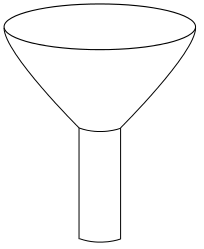
\includegraphics[width=0.25\textwidth]{FIGURES/FilterArray/Filter} & &
\begin{overpic}[scale=.6] %, grid,tics=10]% 
 {FIGURES/Filter}
 \put(20, 70){--, B, --, D, --, --}
\end{overpic} \\
$\Downarrow$ & & $\Downarrow$\\
B & & D \\
\end{tabular}\\
\caption{Example of the two developed arrays}\label{tab:filter}

<<<<<<< HEAD
\end{figure}%
=======
\end{figure}%
>>>>>>> 36a956db0f2ffb15b4b8091da9293464a1b25a0c

\section{Heat Demand and Heat Consumption}\label{sec:result}

In this section we present: (1) the performance of the analysed typologies; (2)
a simple visualization of the result in space (the only part of this analysis
that can be reproduces with the provided data ans scripts); (3) a discussion
regarding the performance of buildings typologies for the analysis of heat
demand in space; (4) a brief discussion on urban typologies and the advantage
of urban typologies over building typologies; and (5) present some possible
implementation of the presented method and future path in our analysis.  We
present a comparison of the typologies and analysed their performance in a
small urban area in the city of Hamburg, Germany. We use this urban area
because we have access to gas consumption data for this area, supplied as part
of a monitoring program, making it possible to analyse the performance of the
different typologies for the estimation of heat demand.\\

The monitoring data is suboptimal for this analysis but is the only data we
have access to for an urban area for which we also have data regarding the
characteristics of the building stock. The monitoring data consists of gas
consumption data given as consumed volume of gas, this has been transformed to
heat consumption data. The mayor problem of this data set for the analysis of
the performance of building typologies for the estimation of heat demand is the
aggregation format. The data set records monitoring points, each point
represents a group of buildings, the building groups contain both residential
and non residential buildings. The building typologies analyzed in this paper
are calibrated to estimate the residential part of the building stock only.
Because we know which building is in each group we can at least know what
percent of the heated area corresponds to the residential sector. This makes it
possible to weight the observation points by heated residential floor area.\\

\subsection{Performance of the Individual Typologies}

In order to quantify the performance of the individual typologies we calculate
the relative difference between consumption and demand for each single
monitoring point, defined as $Wd$.  The weighted mean of the single monitored
points serves as a parameter to define the performance of the typologies and
compare them, see Equation~\ref{eq:diff}.  The mean is weighted by the share of
residential floor space per aggregation level (monitoring point), define by
$r_i$. The share of residential floor space is simple calculated as the
percentage of residential floor space form the total estimated floor space in
that monitoring point.  So for example if a given monitoring point has only non
residential buildings $r_i = 0$ the difference between consumption and demand
for that given point will not be considered for the weighted mean.\\

This method performs relatively good for this particular urban area but might
not be the best approach for other urban areas with a larger and more energy
intensive nor residential building stock. The floor space of buildings is good
indicator for heat demand of the residential sector, but might not be adequate
as an indicator of gas consumption for the non residential sector. A small
business might be using large quantities of gas for more than just heating in
this case the weighting by floor space would not be enough for the performance
analysis of building typologies. On this specif area the non residential
buildings do not affect the overall performance of the individual typologies,
Figure~\ref{fig:con_dem_Residential} shows the result for monitoring points
which contain exclusively residential buildings and the resulting weighting
mean. Although the figures are different the performance of the individual
typologies follows the same order as with the sample containing non residential
buildings.\\ 

\begin{equation} \label{eq:diff}
Wd = 1 \div n \sum_i^n C_i \div D_i \times R_i
\end{equation} 

Where
$C$ represent the  monitored gas consumption for measure point $i$, 
$D$ represents the verage (1000 iterations) heat demand aggregated to point
$i$ and $R$ represents the share of residential floor space in point
$i$\\

We present four results from the typologies comparison as: (1) the relative
difference between demand and consumption wighted by share of residential floor
area (see Table~\ref{tab:diff}); (2) the difference of the sum of demand and
consumption for the entire analysed area (see Table~\ref{tab:diffAbs}); (3) the
percentage of measuring points for which the developed algorithm over estimated
heat demand (see Table~\ref{tab:diffOver}); and (4) deviation of a weighted
Z-statistic (see Table~\ref{tab:WSZ}).  In all four tables we present the
results for both types of arrays \textbf{(B) binary} and \textbf{(F) float},
for three limit values $l$. These limit values define the maximum value taken
into account for the analysis. These limit allows us to differentiate the
performance of the typology for different consumption levels.\\

In addition to both tables we present the comparison between consumption and
demand for all five typologies in form of tree graphs: (1)
Figure~\ref{fig:con_dem_W07} shows the comparison limited to values below
$1e+07$; (2) Figure~\ref{fig:con_dem_W06} shows the comparison limited to
values below $1e+06$; and (3) Figure~\ref{fig:con_dem_Residential} shows the
comparison between estimated heat demand and monitored gas consumption for all
monitored point with exclusively residential buildings limited to values below
$1e+06$.  The first observation in these plots is a clear over estimation of
the heat demand, This overestimation disappears when filtering monitoring
points with non residential buildings on them. This overestimation may relay
not on the typologies itself but on the estimation of floor space of the
individual buildings (see Equation~\ref{eq:space}) as the total heat demand is
computed by multiplying the specific heat demand of the assigned type by the
estimated living space. Another alternative explanation could be achieve by
looking at the climate conditions at the specific monitored year. The monitored
year may have been as especially warm year, making the heat consumption lower
than the average, for which the typologies are designed. As the aim of this
paper is to compare the performance between typologies the overall performance
of the typologies plays a secondary roll in this analysis.\\

\begin{equation}\label{eq:wsz}
  Z =1 \div n\sum_i^n \cfrac{d_i-c_i}{\sqrt{ \left \|
  	  \cfrac{c_i-\left(1-c_i\right)}{\sum{D_i \times r_i}}
  	  \right \|
  	  }}
\end{equation}

\begin{equation} \label{eq:wsz-p}
  c = \frac{C_i}{\sum_i{C_i}}
\end{equation} 

\begin{equation} \label{eq:wsz-E}
  d = \frac{D_{i} \times r_{i}}{\sum_i{\left(D_{i} \times r_{i}\right)
  }}
\end{equation}

Where
$C_i$ represents the monitored gas consumption for measured point $i$,
$D_i$ the estimated heat demand aggregated to measure point $i$ and
$r_i$ the share of non residential floor space in measure point $i$\\

% \begin{figure}[htb]
% \begin{tabular}{lccc}
% \multirow{4}*{
% \begin{sideways}
% Monitored gas consumption $[kWh/a]$
% \end{sideways}
% }
% &a) Blesl S & b) IWUde S & c) IWUhe S\\
% &\includegraphics[width= 0.28\linewidth]{FIGURES/Btyp/Blesl_S07}&
%  \includegraphics[width= 0.28\linewidth]{FIGURES/Btyp/IWUde_S07}&
%  \includegraphics[width= 0.28\linewidth]{FIGURES/Btyp/IWUhe_S07}\\
% &d) BSU S& e) EcoFYS S&
% \multirow{3}*{
% \begin{tabular}{lr}
% \\ \\
% \hline \addlinespace
%  a) Blesl  S & 3.36 \%\\
%  b) IWUde  S & 3.15 \%\\
%  c) IWUhe  S & 3.23 \%\\
%  d) BSU    S & \\
%  e) EcoFYS S & \\ 
% \addlinespace \hline
% \end{tabular}}
% \\ \vspace{-0.3cm}
% &\includegraphics[width= 0.28\linewidth]{FIGURES/Btyp/BSU_S07}&
%  \includegraphics[width= 0.28\linewidth]{FIGURES/Btyp/EcoFYS_S07}\\
% &\multicolumn{3}{l}{Estimated heat demand $[kWh/a]$}\\
% 
% \end{tabular}	
% 	\caption[consumption vs. demand with binary array]
% 	{Shows the monitored consumption of the measuring points
% 	and the computed demand aggregated at the same level (gas consumption measuring
% 	point) uning the binary array}
%     \label{fig:con_dem_S}
% \end{figure}

% \begin{figure}[htb]
% \begin{tabular}{lccc}
% \multirow{4}*{
% \begin{sideways}
% Monitored gas consumption $[kWh/a]$
% \end{sideways}
% }
% &a) Blesl S & b) IWUde S & c) IWUhe S\\
% &\includegraphics[width= 0.28\linewidth]{FIGURES/Btyp/Blesl_S06}&
%  \includegraphics[width= 0.28\linewidth]{FIGURES/Btyp/IWUde_S06}&
%  \includegraphics[width= 0.28\linewidth]{FIGURES/Btyp/IWUhe_S06}\\
% &d) BSU S& e) EcoFYS S&
% \multirow{3}*{
% \begin{tabular}{lr}
% \\ \\
% \hline \addlinespace
%  a) Blesl  S & 3.36 \%\\
%  b) IWUde  S & 3.15 \%\\
%  c) IWUhe  S & 3.23 \%\\
%  d) BSU    S & \\
%  e) EcoFYS S & \\ 
% \addlinespace \hline
% \end{tabular}}
% \\ \vspace{-0.3cm}
% &\includegraphics[width= 0.28\linewidth]{FIGURES/Btyp/BSU_S06}&
%  \includegraphics[width= 0.28\linewidth]{FIGURES/Btyp/EcoFYS_S06}\\
% &\multicolumn{3}{l}{Estimated heat demand $[kWh/a]$}\\
% 
% \end{tabular}	
% 	\caption[consumption vs. demand with flooat array]
% 	{Shows the monitored consumption of the measuring points
% 	and the computed demand aggregated at the same level 
% 	(gas consumption measuring point) using the binary array, 
% 	For values values lower than $1e+06$}
%     \label{fig:con_dem_W06}
% \end{figure}

\begin{figure}[htb]
\begin{tabular}{lccc}
\multirow{4}*{
\begin{sideways}
Monitored gas consumption $[kWh/a]$
\end{sideways}
}
&(a) Blesl & (b) IWUde & (c) IWUhe\\
&\includegraphics[width= 0.28\linewidth]{FIGURES/Blesl_07}&
 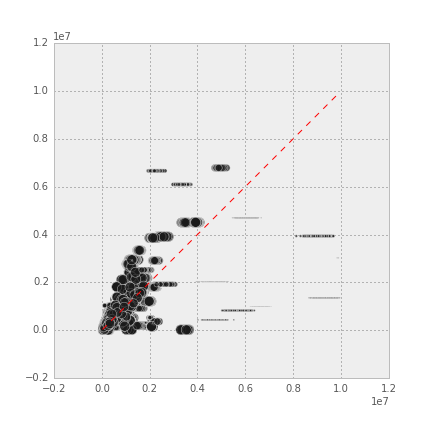
\includegraphics[width= 0.28\linewidth]{FIGURES/IWUde_07}&
 \includegraphics[width= 0.28\linewidth]{FIGURES/IWUhe_07}\\
&(d) BSU & (e) EcoFYS &
\multirow{3}*{
 \begin{tabular}{lr}
 \multicolumn{2}{r}{$l = 1e+07$}\\
 \hline \addlinespace
(a) Blesl   & 0.78 \\
(b) IWUde   & 0.88 \\
(c) IWUhe   & 0.66 \\
(d) BSU     & 0.68 \\
(e) EcoFYS  & 0.72 \\
\addlinespace \hline
\end{tabular}}
\\ \vspace{-0.3cm}
&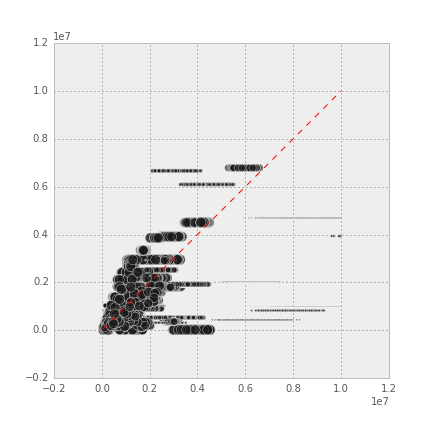
\includegraphics[width= 0.28\linewidth]{FIGURES/BSU_07}&
 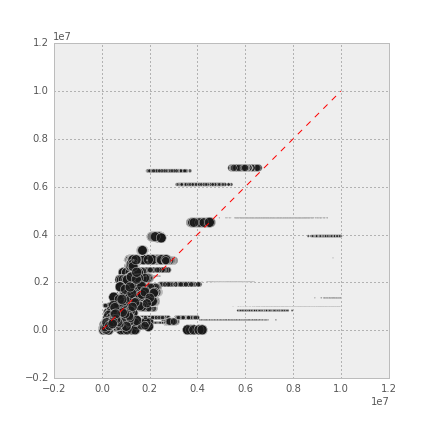
\includegraphics[width= 0.28\linewidth]{FIGURES/EcoFYS_07}\\
&\multicolumn{3}{l}{Estimated heat demand $[kWh/a]$}\\
 
\end{tabular}	
 	\caption[consumption vs. demand with flooat array]{
 	Shows the monitored consumption of the measuring points
 	and the computed demand aggregated at the same level (gas consumption measuring
 	point) using the float array,
 	For values values lower than $1e+06$}
     \label{fig:con_dem_W07}
\end{figure}

\begin{figure}[htb]
\begin{tabular}{lccc}
\multirow{4}*{
\begin{sideways}
Monitored gas consumption $[kWh/a]$
\end{sideways}
}
&(a) Blesl & (b) IWUde & (c) IWUhe \\
&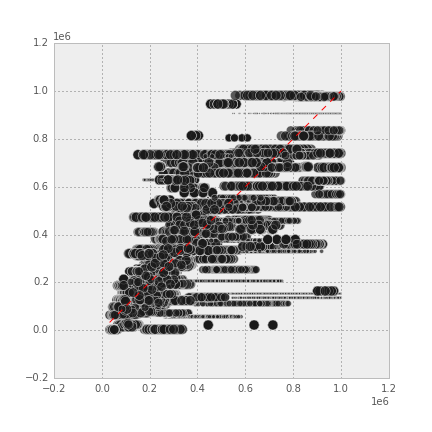
\includegraphics[width= 0.28\linewidth]{FIGURES/Blesl_06}&
 \includegraphics[width= 0.28\linewidth]{FIGURES/IWUde_06}&
 \includegraphics[width= 0.28\linewidth]{FIGURES/IWUhe_06}\\
&(d) BSU & (e) EcoFYS &
\multirow{3}*{
\begin{tabular}{lr}
\multicolumn{2}{r}{$l = 1e+06$}\\
\hline \addlinespace
(a) Blesl   & 0.86 \\
(b) IWUde   & 0.87 \\
(c) IWUhe   & 0.74 \\
(d) BSU     & 0.74 \\
(e) EcoFYS  & 0.77 \\
\addlinespace \hline
\end{tabular}}
\\ \vspace{-0.3cm}
&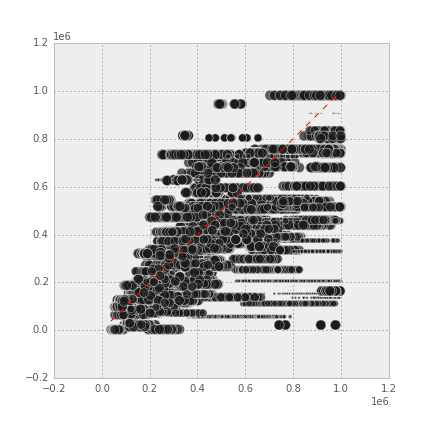
\includegraphics[width= 0.28\linewidth]{FIGURES/BSU_06}&
 \includegraphics[width= 0.28\linewidth]{FIGURES/EcoFYS_06}\\
&\multicolumn{3}{l}{Estimated heat demand $[kWh/a]$}\\

\end{tabular}	
	\caption[consumption vs. demand with flooat array]
	{Shows the monitored consumption of the measuring points
	and the computed demand aggregated at the same level 
	(gas consumption measuring point) using the float array, 
	For values values lower than $1e+06$}
    \label{fig:con_dem_W06}
\end{figure}

\begin{figure}[htb]
\begin{tabular}{lccc}
\multirow{4}*{
\begin{sideways}
Monitored gas consumption $[kWh/a]$
\end{sideways}
}
&(a) Blesl & (b) IWUde & (c) IWUhe \\
&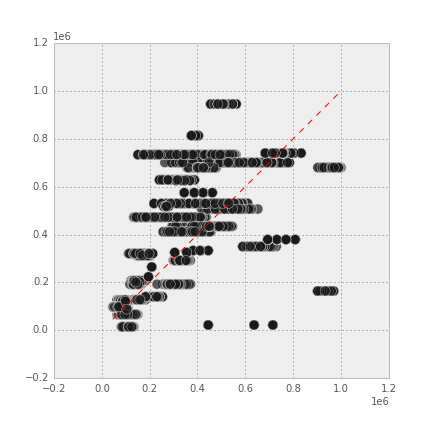
\includegraphics[width= 0.28\linewidth]{FIGURES/Blesl-R_06}&
 \includegraphics[width= 0.28\linewidth]{FIGURES/IWUde-R_06}&
 \includegraphics[width= 0.28\linewidth]{FIGURES/IWUhe-R_06}\\
&(d) BSU & (e) EcoFYS &
\multirow{3}*{
\begin{tabular}{lr}
\multicolumn{2}{r}{$l = 1e+06$}\\
\hline \addlinespace
(a) Blesl   & 1.20 \\
(b) IWUde   & 1.23 \\
(c) IWUhe   & 1.11 \\
(d) BSU     & 1.11 \\
(e) EcoFYS  & 1.13 \\
\addlinespace \hline
\end{tabular}}
\\ \vspace{-0.3cm}
&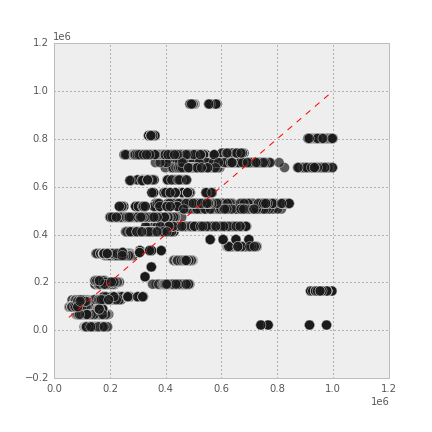
\includegraphics[width= 0.28\linewidth]{FIGURES/BSU-R_06}&
 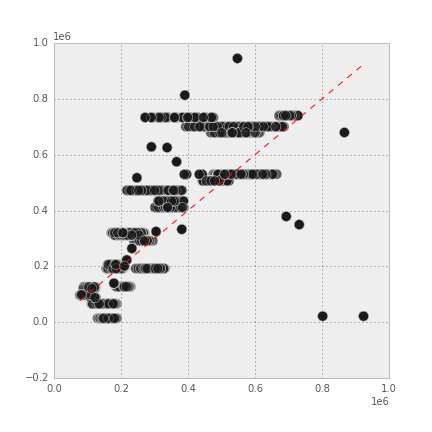
\includegraphics[width= 0.28\linewidth]{FIGURES/EcoFYS-R_06}\\
&\multicolumn{3}{l}{Estimated heat demand $[kWh/a]$}\\

\end{tabular}	
	\caption[consumption vs. demand with flooat array (residential buildings)]
	{Shows the monitored consumption of the measuring points
	and the computed demand aggregated at the same level 
	(gas consumption measuring point) using the float array, 
	For values values lower than $1e+06$ and measuring point with only
    residential buildings.}
    \label{fig:con_dem_Residential}
<<<<<<< HEAD
\end{figure}
=======
\end{figure}
>>>>>>> 36a956db0f2ffb15b4b8091da9293464a1b25a0c

\begin{table}[htb]
\centering
\caption{Average relative difference between demand and consumption
for three different limit points $l$ }
\label{tab:diff}
\begin{tabular}{l ll ll ll}
\toprule
 & \multicolumn{2}{c}{$l = 1e+05$} 
 & \multicolumn{2}{c}{$l = 1e+06$} 
 & \multicolumn{2}{c}{$l = 1e+07$} 
   \\
& B & F & B & F & B & F\\
\midrule
% Blesl  	& .78 & .78 & .74 & .73 & .42 & .41\\
% IWUde  	& .81 & .80 & .76 & .76 & .42 & .42\\
% IWUhe  	& .66 & .66 & .63 & .62 & .36 & .35\\
% BSU		& .67 & .67 & .61 & .61 & .32 & .32\\
% EcoFYS 	& .71 & .71 & .64 & .64 & .33 & .33\\
% Blesl  	& 1.09 & 1.09 & 0.98 & 0.99 & 0.53 & 0.55\\
% IWUde   & 1.12 & 1.12 & 1.01 & 1.02 & 0.54 & 0.55\\
% IWUhe   & 0.95 & 0.95 & 0.85 & 0.86 & 0.46 & 0.47\\
% BSU     & 0.94 & 0.94 & 0.81 & 0.81 & 0.42 & 0.42\\
% EcoFYS  & 0.98 & 0.98 & 0.86 & 0.86 & 0.43 & 0.43\\

(a) Blesl  &  0.75 &  0.79 &  0.87 &  0.86 &  0.79 &  0.78 \\
(b) IWUde  &  0.77 &  0.82 &  0.89 &  0.87 &  0.81 &  0.81 \\
(c) IWUhe  &  0.81 &  0.79 &  0.76 &  0.74$^*$ &  0.67$^*$ &  0.66$^*$ \\
(d) BSU    &  0.72 &  0.72 &  0.74$^*$ &  0.74$^*$ &  0.69 &  0.68 \\
(e) EcoFYS &  0.70$^*$ &  0.69$^*$ &  0.77 &  0.77 &  0.72 &  0.72 \\

\bottomrule
\end{tabular}
\end{table}

\begin{table}[htb]
\centering
\caption{Absolute difference between monitored gas consumption and estimated
    heat demand in $[GWh]$ }
\label{tab:diffAbs}
\begin{tabular}{l ll ll ll}
\toprule
 & \multicolumn{2}{c}{$l = 1e+05$} 
 & \multicolumn{2}{c}{$l = 1e+06$}
 & \multicolumn{2}{c}{$l = 1e+07$}
   \\
& \multicolumn{1}{c}{B} & \multicolumn{1}{c}{F} & 
  \multicolumn{1}{c}{B} & \multicolumn{1}{c}{F} & 
  \multicolumn{1}{c}{B} & \multicolumn{1}{c}{F} \\
\midrule
%Blesl	&  73.64 &  99.62 &  77.68 &  86.61 & 7.74 & 7.93\\
%IWUde	&  56.57 &  83.83 &  71.85 &  81.71 & 7.28 & 7.35\\
%IWUhe	&  60.81 & 108.23 &  83.35 &  98.04 & 8.18 & 8.15\\
%BSU		& 172.30 & 172.88 & 125.76 & 126.48 & 8.74 & 8.73\\
%EcoFYS	& 129.04 & 129.33 & 105.24 & 105.73 & 8.73 & 8.72\\

(a) Blesl  &  0.23 &  0.17 &  21.29 &  21.49 &  178.74 &  169.30 \\
(b) IWUde  &  0.24 &  0.17 &  22.73 &  22.93 &  180.13 &  168.22 \\
(c) IWUhe  &  0.09 &0.08$^*$ &17.92$^*$ &18.10$^*$ &168.02$^*$ &161.73$^*$ \\
(d) BSU    &  0.10 &  0.10 &  23.72 &  23.58 &  192.44 &  192.29 \\
(e) EcoFYS &  0.08$^*$ &  0.08$^*$ &  22.96 &  23.00 &  176.75 &  177.03 \\

\bottomrule
\end{tabular}
\end{table}

\begin{table}[htb]
\centering
\caption{Percentage of over estimated observations}
\label{tab:diffOver}
\begin{tabular}{l ll ll ll}
\toprule
 & \multicolumn{2}{c}{$l = 1e+05$}
 & \multicolumn{2}{c}{$l = 1e+06$}
 & \multicolumn{2}{c}{$l = 1e+07$}
   \\
 & \multicolumn{1}{c}{B} & \multicolumn{1}{c}{F} & 
   \multicolumn{1}{c}{B} & \multicolumn{1}{c}{F} & 
   \multicolumn{1}{c}{B} & \multicolumn{1}{c}{F} \\
\midrule
%Blesl	& .52 & .53 & .60 & .58 & .84 & .84\\
%IWUde	& .47 & .47 & .54 & .54 & .84 & .84\\
%IWUhe	& .59 & .59 & .68 & .67 & .88 & .84\\
%BSU		& .69 & .69 & .76 & .76 & .92 & .92\\
%EcoFYS	& .65 & .65 & .74 & .74 & .92 & .92\\

(a) Blesl &0.56     &0.50     &0.49     &0.51     &0.53     &0.53 \\
(b) IWUde &0.50     &0.43     &0.45$^*$ &0.47$^*$ &0.47$^*$ &0.48$^*$ \\
(c) IWUhe &0.25$^*$ &0.50     &0.65     &0.69     &0.66     &0.68 \\
(d) BSU   &0.50     &0.50     &0.69     &0.68     &0.69     &0.69 \\
(e) EcoFYS&0.33     &0.33$^*$ &0.66     &0.66     &0.64     &0.64 \\

\bottomrule
\end{tabular}
\end{table}

\begin{table}[htb]
\centering
\caption{Weighted sum of Z-statistic deviation of the individual typologies}
\label{tab:WSZ}
\begin{tabular}{l rr rr rr}
\toprule
 & \multicolumn{2}{c}{$l = 1e+05$}
 & \multicolumn{2}{c}{$l = 1e+06$}
 & \multicolumn{2}{c}{$l = 1e+07$}
 \\
 & \multicolumn{1}{c}{B} & \multicolumn{1}{c}{F} & 
   \multicolumn{1}{c}{B} & \multicolumn{1}{c}{F} & 
   \multicolumn{1}{c}{B} & \multicolumn{1}{c}{F} \\
\midrule
% Blesl	& -13.39& -17.06& -20.49& -23.09&   5.29&   5.79\\
% IWUde	& -13.11& -16.99& -20.61& -23.08&   4.00&   4.37\\
% IWUhe	& - 7.20& -13.19& -18.05& -22.69&   1.18&   0.88\\
% BSU		& -21.65& -21.74& -27.61& -28.14& - 0.04& - 0.10\\
% EcoFYS	& -18.17& -18.25& -23.83& -24.30&   4.35&   4.50\\
% Blesl	& -76.46& -78.95& -70.08& -76.94& - 825.76& -  708.57\\
% IWUde	& -72.68& -73.73& -67.95& -73.07& -1983.75& - 1376.57\\
% IWUhe	& -82.53& -89.89& -76.14& -84.06& -3534.62& -12094.36\\
% BSU		& -79.41& -78.93& -72.56& -71.83& -1973.63& - 2022.98\\
% EcoFYS	& -75.54& -74.98& -71.30& -70.59& -5726.72& - 4507.83\\

(a) Blesl  &   -2.55 &   -2.04 &  -0.03 &  -0.03 &  -0.14 &  -0.15 \\
(b) IWUde  &   -3.93 &   -3.17 &  -0.03 &  -0.03 &  -0.14 &  -0.15 \\
(c) IWUhe  &  -20.40 &  -20.57 &  -0.03 &  -0.04 &  -0.22 &  -0.23 \\
(d) BSU    &  -24.02 &  -24.30 &  -0.05 &  -0.05 &  -0.17 &  -0.17 \\
(e) EcoFYS &  -50.48 &  -50.44 &  -0.05 &  -0.05 &  -0.16 &  -0.16 \\

\bottomrule
\end{tabular}
<<<<<<< HEAD
\end{table}
=======
\end{table}
>>>>>>> 36a956db0f2ffb15b4b8091da9293464a1b25a0c


The result from this analysis shows little variation between typologies. This
is very interesting because the underlaying data and methodology for the
construction of the typologies differ between the typologies. While the
typology from~\cite{Blesl.2002} does not use any consumption values for the
construction of the building typology the IWUde typology~\cite{IWU.2003} used
data from the entire country. The performance of the EcoFYS typology does not
perform significantly better than the other typologies but uses Hamburg
specific data for the construction of the typology.\\

The result from our first analysis, comparing the performance of the typologies
by the weighted mean difference between estimated heat demand and monitored gas
consumption, show little variation between the typologies. The use of the float
array has an small effect on the typologies that provide more background
information, needed for the classification with the float array. In the case of
the BSU typology, that provides little background information, the use of the
float typology has almost no impact on the performance of the typology.\\

As expected both typologies developed for the city of Hamburg (BSU and EcoFYS)
achieve the best performance. This good performance applies only for
consumption levels lover than $1e+05 kWh/a$, for the higher consumption levels
the best performing typology is the IWU-he typology.\\ 

For the absolute difference between consumption and demand we observe the same
pattern, for low consumption levels the typologies constructed for Hamburg
outperform the ones constructed for Germany. At a higher consumption level the
IWU-he typology performs best.\\

The percentage of estimation points that where overestimated follows a
different pattern. Typology IWU-de has the lowest share of overestimated points
among all typologies. The shear of overestimated points does not vary much with
a change in consumption level for this typology.
The share of overestimated points can be explain by the non residential sector.
The share of overestimated points reduced drastically by analysing only
monitoring points with only residential buildings. For monitoring points with
only residential sector we see the opposite pattern, the building typologies
underestimate heat demand.\\

The Z-statistic gives us a sense of the typology performance at a individual
level rather that the overall performance of the typology. The performance at
an individual level shows that the typologies constructed for Germany out
performed the typologies design for Hamburg.\\

We identify five points of action in order to increase the performance of
building typologies for the estimation of heat demand at low aggregation level:

\begin{enumerate}
    \item The number of typologies is not enough to distinguish relevant
        building characteristics at a low level of aggregation, we need a more
        precise classification of the building stock.
    \item The typologies do not consider user influence on the consumption of
        heat demand, we argue for the integration of demographic
        characteristics of the occupants for a specif consideration of user
        behaviour in the computation of heat demand.
        See~\cite{MunozHidalgoPeters.2014} for the allocation of families to
        the building stock and~\cite{MunozHidalgo.2014} for the integration of
        user behaviour in urban heat demand models.
    \item The used data for the construction of the typologies is rarely
        monitored heat consumption but estimated values. We pledge the
        community to for a transparent and open share of monitored data for the
        construction of better building typologies.
    \item There is much room for improvement for the classification of the
        building stock. We see this endeavour as part of our ongoing research.
        Available analysis tools can be use for a better classification of the
        building stock, an improvement of the classification can improve the
        performance of these building typologies.
    \item The building typologies are design for the estimation of yearly heat
        demand. In order to estimate heat demand at a lower temporal resolution
        the user has to perform their own heat balance for each individual
        building. In this case the use of the building types is not the
        primary data set but the underlying values of the building components
        (U-values, share of glassing, etc.). We need a typology design for this
        specific cases.
\end{enumerate}

For the proper classification of the building stock plays a significant roll in
the accurate estimation of heat demand in small urban areas. The use of a
digital cadastre for this classification presents itself as a great data
source, to achieve a good classification, unfortunately this data source alone
is not enough for a proper classification of the building stock.\\

We want to develop methods to enrich the digital cadastre previous to the
classification of the building stock. We identify two key parameters for the
classification of the buildings stock and for the estimation of heat demand:
(1) construction year; and (2) floor space.  The proper estimation of
construction year would reduce the uncertainty of the classification procedure.
The second parameter, floor space, is extremely important for the estimation of
heat demand because building typologies provide an specific value for heat
demand in $[kWh/m^2a]$ we multiply this value by the ``heated space'' to
estimate absolute heat demand in $[kWh/a]$.\\

The resulting temporal resolution achieve with this method is not enough to
perform an appropriate heat planing distribution strategy. None of these
typologies are constructed for the estimation of heat demand a lower resolution
level. There is a need for another type of typologies addressing this issue.\\

\subsection{Visualizing the Result in Space}

The visualization of the computed result in space may help us understand the
problems of the developed algorithm.  For this propose we present two maps (see
Figure~\ref{fig:mapsConDem}): (1) showing the estimated absolute heat demand
for the single buildings using the EcoFYS typology; and (2) showing all the
buildings connected to the gas grid for which we have the monitored consumption
values at an aggregated level.  See Section~\ref{sub-sec:data} for details on
data sources.\\

We have identify two important observations in these maps: (1) an over
estimated heat demand for non residential buildings, agglomerated in the north
part of the map; and (2) a possible identification of ``heat spots'' in urban
areas.  These two observations are particular interesting. The first may
explain an overestimation of the heat demand for some of the monitored points
and the second one presents an interesting application of this method.  We
briefly discuss the first observation in the next subsection
(Sub-Section~\ref{sub-section:NR}) making the argument for the need to expand
this analysis to the non residential sector.  In the subsequent section
(Sub-Section~\ref{sub-section:next}) we discuss the further implementation of
the analysis and discuss further paths to expand this method.\\

% \begin{landscape}
% \begin{figure}[htb]
% 	%\caption{Ergebnisse erste Iteration, spezifische W\"armebedarf. Berechnet 
% 	% mit Geb\"audetypologien}
% 	\centering
% 	\includegraphics[height=0.9\textheight]{FIGURES/Btyp/HH}
% 	\caption{Detail from results from the first iteration showing specific heat
% 		demand using buildings typologies}
% \end{figure}
% \end{landscape}
% 
% \begin{landscape}
% \begin{figure}[htb]
% 	% \caption{Ergebnisse erste Iteration, spezifische W\"armebedarf. Berechnet 
% 	% mit Geb\"audetypologien}
% 	\centering
% 	\includegraphics[height=0.9\textheight]{FIGURES/Btyp/Kirchdorf_b}
% 	\caption{Detail of results from the first simulation iteration, showing heat
% 		density for selected urban area using building typologies}
% \end{figure}
% \end{landscape}

\begin{figure}
\begin{tabular}{p{0.5\linewidth}p{0.5\linewidth}} 
\def\svgwidth{\linewidth}
	\import{FIGURES/}{MapHeatDemandEco.pdf_tex}&
\def\svgwidth{\linewidth}
	\import{FIGURES/}{MapGasConsumption.pdf_tex}\\
\end{tabular}
\begin{footnotesize}
\textbf{(a)} Map showing the estimated heat demand in $MWh$ using typology
EcoFYS. 
The red circles mark:
(1) an over estimation of heat demand for non residential buildings; and
(2) identification of a (residential) heat spot in the urban area. 
\textbf{(b)} Map showing the buildings connected to the gas grid (pink)\\
\end{footnotesize}
% 	\label{fig:map-Blesl}
\caption{Maps showing the estimated heat demand and the monitored gas
consumption}
\label{fig:mapsConDem}
<<<<<<< HEAD
\end{figure}
=======
\end{figure}
>>>>>>> 36a956db0f2ffb15b4b8091da9293464a1b25a0c

\subsection{The Need to Include Non Residential Building in the Analysis Scope}\label{sub-section:NR}

Many of the developed typologies have extended their approach to the tertiary
sector~\cite{Loga.2011, Hermelink.2011}, as it is this sector that will be
mixed in urban areas with the residential sector. An estimation of the
industrial sector will differ to much from the typology approach in order to be
include into this methodology. A different approach is presented
by~\cite{Blesl.2007}, in which the authors attempt to classify the tertiary
sector by the required temperature of the processes within the building.  This
approach is very interesting, and an automatic classification of buildings by
the driving needed temperature may be possible thanks to the comprehensive
classification of building use in the digital cadaster (231 classes).  A
parallel comprehensive classification of building uses and their corresponding
energy demand was developed by~\cite{Zeine.2007}.  The connection of these both
data sets may be an interesting option for the estimation of non residential
buildings.\\

Another interesting alternative, specially for urban setting without a
comprehensive digital cadaster, can be the use of urban typologies.  These
typologies will give a specific heat demand for a small group of buildings
without excluding the tertiary sector.  The main aim of building typologies is
to promote and encourage energy efficiency by retrofitting the building
stock~\cite{Loga.2010}.  Because of that, the building typologies focus only on
single buildings rather than on urban areas, targeting the building owners
rather than the energy supply system.  If the aim of the analysis relies not on
the single buildings but on entire urban areas taking into account not only the
single heat demand of the buildings but the underlying infrastructure
supporting the area, a more holistic approach may be useful. \citet{Roth.1980}
developed an urban typology design for the dimensioning of district heating
systems. In Germany and Switzerland, the use of urban typologies for the
description of the building stock and the underlying infrastructure has a long
tradition. For the use of urban typologies in relationship with: (1) heat
supply, see~\cite{Roth.1980, Sieverts.1980, Blesl.2002, Jentsch.2008}; (2) for
the estimation of the potential of solar power generation,
see~\cite{Everding.2004}; (3) a general description of the potential for
renewable energies in open spaces, see~\cite{Genske.2009}; (4) transportation
volume estimation and transportation patterns, see~\cite{Marconi.2006,
Krug.2006}; and (5) for a description of general infrastructure networks
see~\cite{Buchert.2004, Ecoplan.2000, Einig.2006, Erhorn.2011}.\\

\subsection{Next Steps --- Expanding the Method}\label{sub-section:next}

In this sub section we discuss the use of building typologies at an European
and global level. We argue the need to work on method rather than on specific
national building typologies, making a focus on available data of the single
countries.  We also make a small excursion to the use of urban typologies for
the estimation of heat demand and highlight the benefits and problems of using
urban typologies rather that building typologies.\\

Having access to a detailed digital cadaster of the city offers a vast set of
possibilities for the simulation of heat demand of urban areas.  A simple
balance of heat demand can be performed without much effort and with a relative
low input of data.  Much of the needed data for a energy balance of a single
building can be recover through the digital cadaster.  The missing data for
such a computation are the U-values of the single building components.  These
building typologies are not constructed for this purpose.  There is an
alternative to the use of building typologies, this is the use of a building
component typology.  For Germany there is a regional material catalog developed
by the Center for Environmental Friendly Construction\footnote{(Zentrum für
    Umweltbewusstes Bauen e.V.)
    \url{http://www.zub-kassel.de/}}~\cite{Klauss.2009}.
With help of this catalog we could simulate heat consumption upon building
components rather than upon building typologies.  First attempts have been
performed by our research team~\cite{Munoz.2014c}. The simulation at such level of
detail may foster further insights on different topics needed for an holistic
understanding of urban systems.  This method could be applied for the
simulation of material flows in urban systems as well as a estimation of
retrofit cost and the construction and demolition waste arising from such
retrofits.\\
%TODO: support with some literature about CDW

%TODO: the use of building typologies for datarecovery
%\cite{Meinel.2008}
% Automatische Ableitung von stadtstrukturellen Grundlagendaten und Integration
% in einem geographischen Informationssystem
% \cite{YiminChen.2011}
% Estimating the relationship between urban forms and energy consumption: A case
% study in the Pearl River Delta, 2005–2008

%% If you have bibdatabase file and want bibtex to generate the
%% bibitems, please use
%%
\section*{Bibliography}
\bibliographystyle{elsarticle-harv} 
\bibliography{/home/esteban/Documents/Bib/Diss.bib}

%\section*{Annex}
%\begin{longtable}{ll | lllllll | lllll | l}

  \centering
  \caption[Building typology - EcoFYZ Parameters (1/2)]{
  Building typology for the city of Hamburg developed by EcoFYZ showing the 
  parameters of each Typ, in percentage.
  \cite[pp.~18]{Hermelink.2011}}
  \label{tab:EcoFYZParam1}%
    \begin{tabular}{ll | lllllll | lllll | l}
    \cmidrule{1-14}
    & Year (BAJ) & \multicolumn{7}{c|}{Floor (AOG)} & \multicolumn{5}{c|}{Roof (DAF)}\\
    &            & \begin{sideways}01--02 \end{sideways}&
    			   \begin{sideways}03--03 \end{sideways}& 
    			   \begin{sideways}04--05 \end{sideways}& 
    			   \begin{sideways}06--09 \end{sideways}&
    			   \begin{sideways}10--13 \end{sideways}&
    			   \begin{sideways}14--15 \end{sideways}&
    			   \begin{sideways}16--20 \end{sideways}& 
					sa & m & w & f & so & %\\
    \multirow{45}{*}{
	\begin{sideways}
	    \begin{minipage}{19cm}
			\begin{footnotesize}
				$^*$ MFH-Hochhaus, massiv.
				(sa) pitched roof, ``Satteldach'';
				(m) curg roof, ``Mansardendach'';
				(w) hip roof, ``Walmdach'';
				(f) flat roof, ``Flachdach'';
				(so) other, ``Sonstiges''.
			\end{footnotesize}
		\end{minipage}
	\end{sideways}
}\\
\cmidrule{1-14}
%\midrule
\multirow{8}{*}{\begin{sideways} Freist. EFH / DHH \end{sideways}}
\multirow{8}{*}{\begin{sideways} Semi detached / \end{sideways}}
\multirow{8}{*}{\begin{sideways} Single family house \end{sideways}}
&\textless~1918     & 94 & 6 & 0 & 0 & 0 & 0 & 0 & 51 & 13 & 26 & 5 & 5 \\ 
&1919--1948  & 99 & 2 & 0 & 0 & 0 & 0 & 0 & 60 & 5 & 26 & 4 & 5 \\ 
&1949--1957  & 99 & 1 & 0 & 0 & 0 & 0 & 0 & 71 & 2 & 19 & 4 & 4 \\ 
&1958--1968  & 98 & 2 & 0 & 0 & 0 & 0 & 0 & 65 & 3 & 20 & 9 & 3 \\ 
&1969--1978  & 99 & 2 & 0 & 0 & 0 & 0 & 0 & 61 & 3 & 24 & 10 & 3 \\ 
&1979--1983  & 99 & 1 & 0 & 0 & 0 & 0 & 0 & 65 & 4 & 22 & 6 & 3 \\ 
&1984--1994  & 99 & 1 & 0 & 0 & 0 & 0 & 0 & 47 & 5 & 42 & 3 & 2 \\ 
&\textgreater~1995     & 98 & 2 & 0 & 0 & 0 & 0 & 0 & 50 & 3 & 36 & 5 & 6 \\ 
\cmidrule{1-14}
\multirow{8}{*}{\begin{sideways} Reihenhaus \end{sideways}}
\multirow{8}{*}{\begin{sideways} Terrace house \end{sideways}}
&\textless~1918     & 84 & 13 & 3 & 0 & 0 & 0 & 0 & 37 & 24 & 14 & 23 & 2 \\ 
&1919--1948  & 95 & 5 & 0 & 0 & 0 & 0 & 0 & 68 & 3 & 19 & 10 & 1 \\ 
&1949--1957  & 99 & 1 & 0 & 0 & 0 & 0 & 0 & 85 & 1 & 2 & 11 & 1 \\ 
&1958--1968  & 100 & 0 & 0 & 0 & 0 & 0 & 0 & 77 & 1 & 1 & 20 & 1 \\ 
&1969--1978  & 97 & 3 & 0 & 0 & 0 & 0 & 0 & 52 & 2 & 1 & 43 & 2 \\ 
&1979--1983  & 96 & 4 & 0 & 0 & 0 & 0 & 0 & 79 & 7 & 1 & 10 & 2 \\ 
&1984--1994  & 98 & 2 & 0 & 0 & 0 & 0 & 0 & 72 & 12 & 9 & 2 & 5 \\ 
&\textgreater~1995     & 76 & 23 & 0 & 0 & 0 & 0 & 0 & 50 & 0 & 6 & 24 & 19 \\ 
\cmidrule{1-14}
\multirow{8}{*}{\begin{sideways} MFH-Einzelhaus \end{sideways}}
\multirow{8}{*}{\begin{sideways} Single family house \end{sideways}}
&\textless~1918     & 49 & 38 & 11 & 1 & 0 & 0 & 0 & 30 & 29 & 25 & 10 & 6 \\ 
&1919--1948  & 69 & 26 & 4 & 0 & 0 & 0 & 0 & 24 & 12 & 53 & 7 & 4 \\ 
&1949--1957  & 68 & 22 & 10 & 1 & 0 & 0 & 0 & 44 & 8 & 28 & 17 & 3 \\ 
&1958--1968  & 68 & 21 & 8 & 3 & 0 & 0 & 0 & 57 & 8 & 13 & 19 & 3 \\ 
&1969--1978  & 59 & 32 & 8 & 0 & 0 & 0 & 0 & 44 & 8 & 12 & 34 & 2 \\ 
&1979--1983  & 65 & 26 & 8 & 1 & 0 & 0 & 0 & 39 & 24 & 15 & 20 & 2 \\ 
&1984--1994  & 72 & 21 & 6 & 1 & 0 & 0 & 0 & 36 & 27 & 24 & 7 & 6 \\ 
&\textgreater~1995     & 48 & 31 & 18 & 2 & 0 & 0 & 0 & 31 & 6 & 22 & 29 & 12 \\ 
\cmidrule{1-14}
\multirow{8}{*}{\begin{sideways} MFH-Wohnblock \end{sideways}}
\multirow{8}{*}{\begin{sideways} Block family house \end{sideways}}
&\textless~1918     & 6 & 19 & 67 & 8 & 0 & 0 & 0 & 19 & 66 & 2 & 11 & 2 \\ 
&1919--1948  & 13 & 26 & 51 & 9 & 0 & 0 & 0 & 29 & 40 & 11 & 18 & 3 \\ 
&1949--1957  & 7 & 25 & 63 & 5 & 0 & 0 & 0 & 51 & 20 & 11 & 17 & 1 \\ 
&1958--1968  & 10 & 25 & 59 & 7 & 0 & 0 & 0 & 48 & 28 & 5 & 18 & 2 \\ 
&1969--1978  & 4 & 22 & 65 & 8 & 0 & 0 & 0 & 34 & 39 & 6 & 19 & 2 \\ 
&1979--1983  & 6 & 23 & 63 & 9 & 0 & 0 & 0 & 35 & 38 & 7 & 17 & 3 \\ 
&1984--1994  & 7 & 23 & 61 & 8 & 0 & 0 & 0 & 34 & 43 & 5 & 14 & 4 \\ 
&\textgreater~1995     & 25 & 31 & 34 & 9 & 0 & 0 & 0 & 30 & 18 & 6 & 38 & 8 \\ 
\cmidrule{1-14}
\multirow{8}{*}{\begin{sideways} MFH-Gruppenhaus \end{sideways}}
\multirow{8}{*}{\begin{sideways} Group family house \end{sideways}}
&\textless~1918     & 6 & 33 & 55 & 6 & 0 & 0 & 0 & 41 & 38 & 10 & 7 & 4 \\ 
&1919--1948  & 8 & 28 & 54 & 10 & 0 & 0 & 0 & 33 & 4 & 37 & 25 & 1 \\ 
&1949--1957  & 12 & 23 & 62 & 3 & 0 & 0 & 0 & 62 & 1 & 20 & 17 & 1 \\ 
&1958--1968  & 17 & 43 & 38 & 3 & 0 & 0 & 0 & 59 & 2 & 4 & 34 & 1 \\ 
&1969--1978  & 12 & 29 & 49 & 9 & 0 & 0 & 0 & 35 & 3 & 11 & 51 & 1 \\ 
&1979--1983  & 12 & 30 & 48 & 10 & 0 & 0 & 0 & 44 & 11 & 11 & 33 & 1 \\ 
&1984--1994  & 19 & 37 & 40 & 5 & 0 & 0 & 0 & 49 & 18 & 15 & 15 & 3 \\ 
&\textgreater~1995     & 14 & 33 & 45 & 9 & 0 & 0 & 0 & 29 & 4 & 13 & 45 & 9 \\ 
\cmidrule{1-14} 
\multirow{2}{*}{\begin{sideways} HH$^*$ \end{sideways}}
&1958--1968  & 0 & 0 & 0 & 55 & 32 & 5 & 6 & 5 & 3 & 0 & 89 & 3 \\ 
&1969--1978  & 0 & 0 & 1 & 39 & 47 & 7 & 6 & 0 & 0 & 0 & 99 & 0 \\
\cmidrule{1-14}
    \end{tabular} 
\end{table}%


\end{linenumbers}
\end{document}

\endinput
